\documentclass[a4paper,12pt]{book}
\usepackage[utf8]{inputenc}
\usepackage[margin=24mm]{geometry}

\usepackage{float}
\usepackage{graphicx}
\graphicspath{ {images/} }

\usepackage[
backend=bibtex,
style=alphabetic,
citestyle=authoryear,
autocite=inline
]{biblatex}

\addbibresource{references/references.bib}

\usepackage{helvet}
\usepackage{subfig}

\usepackage[Lenny]{fncychap}
\usepackage{xcolor}


\begin{document}

\frontmatter
%----------------------------------------------------------------------------------------
%	TITLE PAGE
%----------------------------------------------------------------------------------------

\newcommand*{\titlePage}{\begingroup % Create the command for including the title page in the document
	\fontfamily{phv}\selectfont
	\centering % Center all text
	
	\vspace{200pt}
	{\Huge Developing an educational tool to promote evidence-based treatment in health care} \\ % Title
	\vspace{5pt}
	
	{\Large \textsl{A pilot study}} % Subtitle or further description
	\vspace{50pt}
	
	{\Large{Ben-Richard Sletten Ebbesvik}}\\ % Author name
	
	\vfill % Whitespace between the author name and the publisher logo
	
	{\Large Research proposal for master's thesis in Software Engineering at \\
		\vspace{10pt}
		Department of Computing, Mathematics and Physics, \\
		Bergen University College \\
		\vspace{10pt}
		Department of  Informatics, \\
		University of Bergen \\}
	\vspace{10pt}
	{\large April 2018} % Month and year published
	
	\begin{figure}[h!]
		\captionsetup[subfigure]{labelformat=empty}
		\subfloat[][]{
\includegraphics[width=250pt]{images/hvl_logo_engelsk.pdf}}
		\hfill
		\subfloat[][]{
\includegraphics[width=70pt]{images/uib-logo.pdf}}
	\end{figure}
	
	
	\endgroup}
\titlePage

\newpage
\section*{Abstract}
\newpage
\section*{Acknowledgement}
My supervisors Yngve Lamo and Svein Ivar Lillehaug

Job Nyangena
Fazle Rabbi

Rosaline Barendregt
Suresh Kumar Mukhiya

Idar Syslak
Mohnd Skr
Fredrik Hoel
August Hoel

Nikolai Grieg
Gard Engen

My family Malin, my parents, my brother and his family
\newpage
\begin{flushright}
	\null\vspace{\stretch{1}}
	\itshape
	To Malin \\
	and my parents
	\vspace{\stretch{3}}\null
\end{flushright}

\tableofcontents
\mainmatter

% HUSK Å LEGGE INN LISTE OVER TABELLER, FIGURER OG LISLINGS I INNHOLDSFORTEGNELSEN!!!!

\chapter{Background}

\section{Clinical Practice Guidelines}
\textcite{Fervers2010} claims that for clinicians, increased medical knowledge is associated with an exponential growth of scientific data and published material. It is impossible to keep up, as well as integrating all the new information into daily practice to give patients the best possible care.  \textcite{Masic2008} gives an example where a general practitioner should read 19 articles per day to keep up with the new medical information, while only having time for reading one hour per week. Reading 19 articles per day, would acquire more time than the clinician has available for treating patients. This problem is known as academic isolation \parencite{Masic2008}.

Evidence Based Medicine (EBM) suggests that instead of routinely reading dozens of articles, the clinicians should target their reading to specific patient problems. Developing clinical questions and then searching for the answer (problem based approach) may be a more productive way to keep up with the new medical knowledge \parencite{Masic2008}. The EBM definition further puts an emphasize on integrating the best evidence in decision making with the clinicians expertise and the patients values and expectations \parencite{Masic2008}. 

The concept of EBM is about transferring knowledge from clinical research into clinical practice, and Clinical Practice Guidelines (CPG) can play an instrumental role in this process \parencite{Fervers2010}.

The Institute of Medicine (IOM) has given the following definition of clinical practice guidelines: "CPGs are statements that include recommendations intended to optimize patient care. These statements are informed by a systematic review of evidence and an assessment of the benefits and costs of alternative care options" \parencite{Guidelines2011}

The definition given by IOM covers the goals in EBM, and also takes the cost into account. In fact, \textcite{Clayton1995} have shown that in some situations good use of appropriate guidelines and protocols can reduce as much as 25\% of the cost of healthcare.

% I can use Woolfs article and write even more about benefits. Should probably do that.

Even though the CPGs have proven to improve the quality of health care while reducing practice variability and the cost of patient care \parencite{DeClercq2008}, it is well recognized that CPGs have had a limited effect on changing the clinicians practice methods. \textcite{Cabana1999} lists the following reasons:
\begin{itemize}
	\item \textbf{Lack of awareness:} the clinician is not aware of the guideline's existence.
	\item \textbf{Lack of familiarity:} the clinician is not familiar with the content of the guideline.
	\item \textbf{Lack of agreement:} the clinician had various reasons to disagree with the guideline, such as they are oversimplified, disagree with the evidence or not worth the patient risk, discomfort or cost.
	\item \textbf{Lack of self-efficacy:} is the lack of self-confidence in that the clinician can execute the recommendations of the guideline correctly.
	\item \textbf{Lack of outcome expectancy:} the clinician doesn't believe the outcome of the recommended treatment will meet the outcome expectancy.
	\item \textbf{Inertia of previous practice:} the custom, habit or previous training can hinder the adaptation of clinical practice.
	\item \textbf{External Barriers:} the guidelines are not easy to use, not convenient, cumbersome and confusing.
\end{itemize}One example of external barrier is the Guidelines for the Diagnosis and Management of Asthma \parencite{NationalHeartLungandBloodInstitute2007}, which consists of 440 pages. Such a large document is not convenient to use at the point of care. According to \textcite{Shortliffe1998}, CPGs in monographs and journal articles tend to sit on book shelves at the time their knowledge could prove the most valuable to the clinicians. 

\subsection{Discussion}
According to \textcite{Woolf1999}, clinicians sometimes have good reasons to disagree with some of the content of a guideline. \textcite{Woolf1999} points out three reasons:
\begin{enumerate}
	\item The scientific evidence of the recommendation can be lacking, misleading or misinterpreted.
	\item The recommendations may be influenced by the authors. What the authors believe, may be inferior to other options, ineffective or harmful.
	\item As the guideline may be written to control cost, serve societal needs or protect special interest, the recommendations may be suboptimal for the patient.
\end{enumerate}
There exists grading systems which grade the quality of evidence and strength of recommendations. GRADE is such a grading system \parencite{Guyatt2008}. When displaying guidelines to clinicians, it is a strong point to display the grade of evidence, as the clinician has to choose between several treatment options.


%\textcolor{red}{\begin{itemize}
%	\item Medical knowledge increases. Hard to keep track
%	\item Guidelines is a summary of the available evidence of the medical conditions and provide management and recommendations
%	\item A well-developed guideline reduces
%	variations in care, improves diagnostic accuracy,
%	promotes effective therapy and discourages ineffective
%	therapies all which contribute to improved
%	quality of care (citation)
%	\item The CPGs are not used enough
%	\item Dissemination and implementation
%	\item Large volume of excisting guidelines. Difficult to use at the point of care
%	\item Dissemination
%	\item Different practice even in the same country
%\end{itemize}}


\section{Serious games}
When searching the literature for the definition of serious games, there seem to be many different understandings of what serious games really is. However, these definitions seem to have the common understanding that serious games are games which are used for other purposes than just pure entertainment \parencite{Susi2015}. This is actually a very broad category, where we can find games which are used to test job applicants or to improve our health by encouraging us stay more active.

\textcite{Michael2006} defines serious games as "a serious game in which education (in its various forms) is the primary goal, rather than entertainment". \textcite{Michael2006} emphasizes that education and entertainment should not be in conflict, but that they can overlap. The feeling of learning something new or getting better at something, can be quite satisfying and can serve as an entertainment factor.

Serious games also have the advantage over educational books and movies that the student can demonstrate and apply what he has learnt, through tasks in the game \parencite{Michael2006}.    Serious games seem more effective than training with conventional instruction methods, as the knowledge gains persists in the long term memory, and the learner can build on this well-structured prior knowledge through his learning career \parencite{Wouters2013}. However, serious games seems to be most effective when they are supplemented with instructional learning methods. Not only gets the student to learn by doing, but he also gets the opportunity to reflect over what he has learnt and to verbalize the new knowledge, making it easier to integrate it into his knowledge base \parencite{Wouters2013}. 





\section{Motivation}
By making a serious game for clinical practice guideline training, we can address some of the reasons why the CPGs haven't had a greater impact on clinicians practice methods \parencite{Cabana1999}:
\begin{itemize}
	\item \textbf{Lack of awareness:} The more projects around CPGs, the more focus will they get and more people will be aware of their existence. By making a serious game, we may be able to target some user groups which where hard to reach in traditional ways. 
	\item \textbf{Lack of familiarity:} By playing the game, the student will learn more about the content and will become familiar with the CPGs. The student may also be encouraged to study the CPGs in the traditional ways after having played the game.  
	\item \textbf{Lack of self-efficacy:} By repeatedly solving practical tasks in the game, the student may become confident in that they are capable of executing the treatment recommended by the CPG.
	\item \textbf{External barriers:} convenient, cumbersome and confusing CPGs will by approach be converted to a game format. Even though a game isn't a good encyclopaedia at the point of care, for some user groups a game might be a better format for studying. Especially a combination of instructional learning methods and serious games have shown positive learning results \parencite{Wouters2013}. Having built well-structured prior knowledge may also help at the point of care.
\end{itemize}

Another motivational reason for making a serious game is the scalability. How can we best train 10, 100 or 1000 clinicians in the best practices of medical guidelines? There are logistics problems with instructional courses and training sessions, such as cost of money, time and there's a practical limit for how many attendees can attend a course at the same time. A mobile game scales much better as downloading an mobile application is much cheaper, can be played almost anywhere at any time. There's no limitation on how many playing participants.

\subsection{Asthma}
Asthma is a repository disease, which in the recent years have had an almost exponential growth rate among children in Oslo. From 0.4\% in the first Norwegian report, to 8\% in 1993 and 20.2\% in 2006. Similar results were found in the rest of Norway in the early 90s. \parencite{Carlsen2006}. 

Asthma growth amongst children is not only an issue in Norway. According to \textcite{Odhiambo1998}, 3\% of children in rural areas in Kenya had asthma in 1998 and 9.5\% of the children in urban areas. Before this study it was a claim that asthma among African children was rare, which is no longer true \parencite{Odhiambo1998}.

It is urgent to find answers to prevent further increase of asthma amongst children in the years to come\parencite{Carlsen2006}.

As our contribution to put focus on the dramatically growth of asthma in children, our work will centre around the paediatric possible asthma guideline \parencite{RepublicofKeny2016} when developing a serious game to promote guideline training in health care.

\subsection{Challenges}
\section{Related work}
\section{Summary}

\chapter{Introduction}

\section{Paper publication}
In December 2018, we submitted a paper "A Model Driven Approach to the Development of Gamified Interactive Clinical Practice Guidelines", which was a summary of our work so far in this project and related projects. The paper was accepted for publication by ENASE 2019 – 14th International Conference on Evaluation of Novel Approaches to Software Engineering, where we held a presentation on their conference in Heraklion, Greece. 

The paper can be found in appendix \ref{appendix:Paper} in this thesis.

%\section{Old Research questions}
%\begin{itemize}
	%\item Can we make a data structure representing the paediatric possible asthma guideline \parencite{RepublicofKeny2016}  in a very generic way?
	%\item Based on the data structure, can we generate suitable scenarios, with multiple choice %question with answer elements for training and evaluating health personnel?
	%\item How can we structure the learning material to best train medical students, doctors, clinical officers, nurses and other health workers in the paediatric possible asthma guideline \parencite{RepublicofKeny2016}? 
			%\item Based on clinical guidelines, can we make a reusable data structure representing respiratory diseases for use in serious games?


%-------
%	\item Based on clinical guidelines, can we make a data structure which is easy to implement in the system, as well as adaptable? 
	
%	\item How to use such a model for generating and testing case based multiple choice questions and answer elements?
	%\item Can we use the data model to structure the learning content such that it is adapted to the current knowledge of the individual learner?
	
	
%	\item How can we model the work-flow of a clinical encounter, a patient at a given point in the clinical encounter, and a student at the current point in his learning process. How to represent these?	
%\end{itemize}

%\textcolor{purple}{TODO Yngve: Gamification, hva evaluerer du?}


\section{Research questions}

\begin{itemize}
	\item \textbf{RQ1:} Based on clinical guidelines, how can we define and represent a generic data structure that can be used to implement applications such as online guidelines or training games for such guidelines, and where applications can adapt to the level of their users?
	\item \textbf{RQ2:} Can the generic data structure in RQ1 be used to generate a specific data model for another domain such as paediatric asthma?
	\item \textbf{RQ3:} How can we use the data model in RQ2 to implement a game for guideline training that can adapt to the level and progression  of users?
	\item \textbf{RQ4:} Is the guideline meta model at an abstraction level such that it can be used for other guidelines? 
\end{itemize}
\section{Structure of the thesis}
\section{Summary}
Here we have defined a set of research questions, which is related to the development of serious games for clinical guidelines. Making games which are adaptable to the knowledge level, progression of the user, and making guideline models which are at an abstraction level where they can be used to represent other CPGs, are the main focus points.

We have also given a short presentation of each chapter in the thesis.




\chapter{Method}


\section{Design study}
The research methodology we used for this project was an adaptation of design science \parencite{Hevner2004}.  In short, design science requires an artefact that either solves a an organizational problem. The artefact itself and the construction of it goes through evaluations in iterations, to make sure its relevance to the problem domain. We must ensure that the research contributes value to both the health care domain as well as computer science.

\textcite{Hevner2004} proposed some guidelines design science in information system research. We will go through them and connect them to our research project.

\begin{itemize}
	\item \textbf{Guideline 1: Design as an Artefact.} The artefact will be a serious mobile game with the associated data models.
	\item \textbf{Guideline 2: Problem Relevance.} Clinical Practice Guidelines are improving the quality of health care, reduce practice variability and the cost of health care \parencite{DeClercq2008}. But they have had a limited effect on changing the clinicians practice methods \parencite{Cabana1999}. Some of the reasons \textcite{Cabana1999} lists are that some clinicians are not aware of the guidelines, they are not familiar with the guideline content, as well as the guidelines are difficult to use, cumbersome, inconvenient and confusing. These are issues we can address with a game.
	\item \textbf{Guideline 3: Design Evaluation.} The design process is described in the next section, where each iteration has clear goals and evaluations. Cognitive walkthroughs and usability tests with users are some of the evaluation methods used. In the end of the thesis, we will demonstrate that the datamodels can be used to represent other clinical practice guidelines, as well as evaluating the game with medical experts.
	\item \textbf{Guideline 4: Research Contributions} are our data models, which are the backbone of the game. The data models should be generic enough to represent and make games for other clinical practice guidelines. Adaptable to the user's knowledge level and with flexible learning paths.
	\item \textbf{Guideline 5: Research Rigor} and \textbf{Guideline 6: Design as a Search Process.} The construction of the artefact followed a similar process described in figure \ref{fig:InteractionDesignLifeCycle}. It's an iteratively process where requirements were established through focus group, workshop, studying similar products, talking with domain experts and informal literature studies. Then designing alternatives, which also can be functionality suggested to the artefact. Prototyping was making prototypes or constructing the artefact itself. An evaluation decides whether the new functionality/prototype can be used as it is or update the requirements and make a new version.
	
		\begin{figure}[h!]
		\caption {The project followed a similar process to the life cycle of interaction design. Figure derived from \textcite{Preece2015}}
		\label{fig:InteractionDesignLifeCycle}
		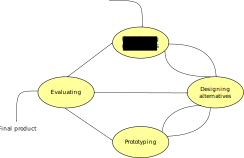
\includegraphics[scale=0.5]{InteractionDesignLifeCycle}
	\end{figure}
	\item \textbf{Guideline 7: Communication of Research,} which is the purpose of this masters thesis. We have also published a paper, which can be found in the appendices.
\end{itemize}


\section{Iterations}


\subsection {Testing mobile app technology, conceptual model}
The goal of this iteration was to make a prototype using the proposed technology. The prototype will tell us if it is sensible to use the technology for the project, as well as having a conceptual model to use when discussing initial ideas around the aim of the project, functionality, as well as interaction design.

The technology to be tested was React Native. The reason for this to be the first choice, was to support multiple platforms and not having to rewrite the application for every platform. The same application can be used for Android and iPhone with little modification to the code. React Native is build upon the React front end web development framework, which means some code can be reused for web as well. But all the the views need to be modified, as they use specific React Native components for mobile units. React and React Native are JavaScript frameworks.

We have also used the React web  development framework in previous projects. It s one of the more popular and mature front end web development frameworks in the market. 

The prototype itself and the development process showed that the technology could be used for displaying and organize CPGs. Lessons learned about content flow, databases, app navigation, displaying information and dialogues. JavaScript in the view gives a lot of flexibility compared to just tags.

\begin{figure}[h!]
	\caption {A very simple conceptual model to test one of the proposed technologies, as well as acting as a starting point for discussions}
	\label{fig:ConseptualModel}
	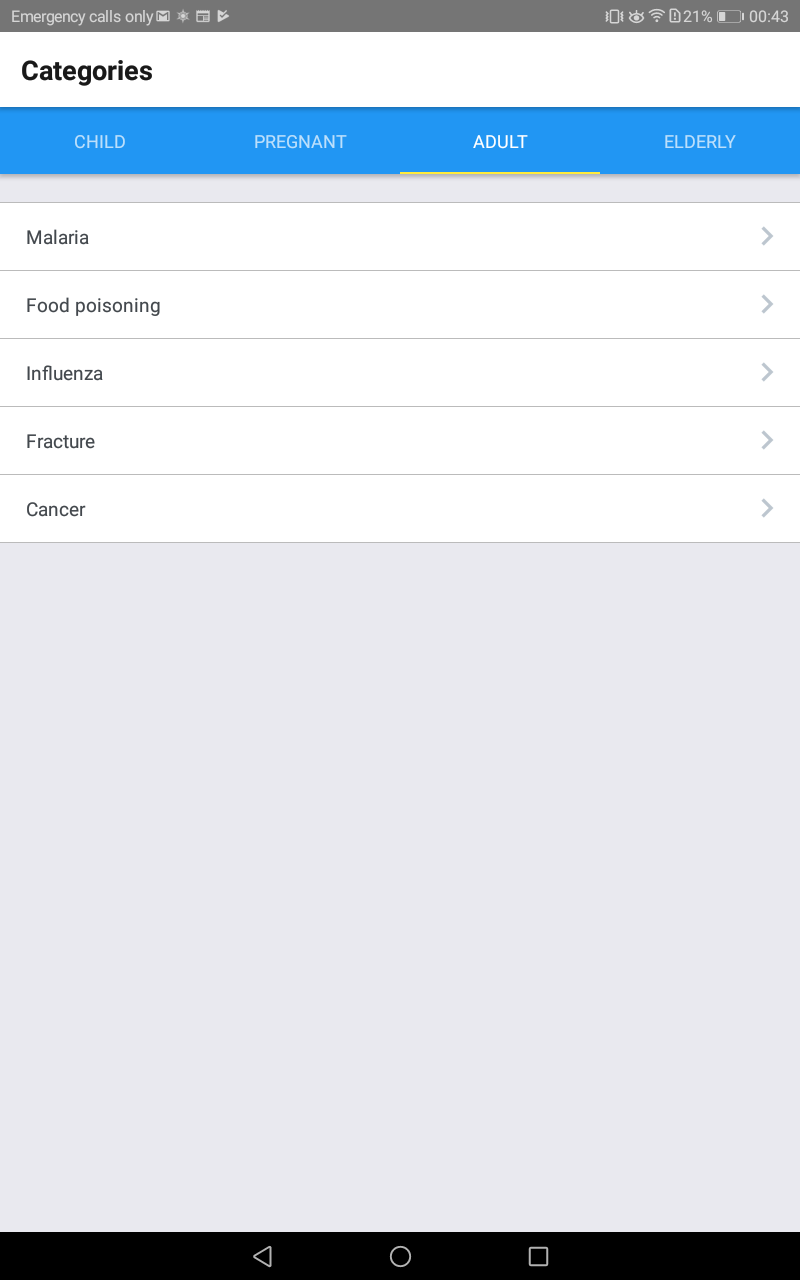
\includegraphics[scale=0.2]{ConceptualPrototype}
\end{figure}

The interface was evaluated with the supervisors, using cognitive walkthroughs. It also worked as a conceptual model, using the prototype as a base for discussing ideas. Both for discussing the purpose of the project, what the user should be able to do, how to organize content and what functionality to add.


\subsection{Studying similar products}
The purpose of the iteration is to see what exists in the market. What have others done. What can we improve, where can we add value to both the medical community and to computer science.

The results from this iteration is presented in appendix \ref{appendix:ComparisonApps}, and was done together with a fellow master of science student in software engineering. As a conclusion, none of these application have a data model which can represent CPGs, nor a patient in a clinical encounter. The representations of CPGs are mostly text based, flow charts or flow charts which expand when you click on decision vertices. LIFE: Neonatal Resuscitation Training is a pretty advanced 3D game, but there is no data model representing the content in the quizzes and tasks.

\subsection{Technology used to represent CPGs}
In this iteration we evaluated technologies which could be used to model CPGs.


\begin{itemize}
	\item \textbf{GLIF} and \textbf{PROforma} was compared during a literature study as a semester assignment in health informatics. We will here give a brief summary of GLIF.
	
	 GLIF or the Guideline Interchange Format, was developed by the InterMed Collaboratory. The intention was to make a guideline representation language, which can be viewed with a various of software application as well as adapting them and making them valid for different local uses. The representation should be precise, ambiguous, readable by humans and interpretable by computers, adaptable to different clinical information standards and facilitating guideline sharing \parencite{Peleg2000}. 

	To make the guidelines readable for humans, interpretable by computers and adaptable by different institutions, GLIF defines the guidelines at three different abstraction levels: conceptual, computable and implementable levels \parencite{DeClercq2008} 
	
	The conceptual level is the highest abstraction level. It consists of
flow-charts which can be viewed by humans, using guideline viewing programs. At this level the guidelines can not
	be used for computations in decision support \parencite{Peleg2000}. 
	
	At the computable level expressions, patient data elements, clinical actions and guideline flow
	are specified at this level. The guidelines can also be verified for logical consistency and completeness \parencite{Peleg2000}.
	
	The implementable level contains the information to incorporate the guidelines into
	the particular institutions knowledge or information system such as EPR \parencite{Peleg2000}.
	
	In figure \ref{fig:GLIFPossibleAsthma} we present a model of the paediatric possible asthma guideline \parencite{RepublicofKeny2016} at the conceptual level. We will now explain the guideline steps the UML-model in figure \ref{fig:GLIFPossibleAsthma} consists of.
	\begin{itemize}
		\item \textbf{Action step} a representation of a recommended tasks or action. There are three types of actions steps: Medically oriented (such as a recommendation for a treatment), programming oriented (such as retrieving information from EHR), control-oriented that invokes nested control structures (subguidelines or macros to support recursive specification) \parencite{DeClercq2008}. Action steps are green squares in figure \ref{fig:GLIFPossibleAsthma}.
		\item \textbf{Decision step} represents a decision point in the model. There are two types of decision steps: Case and Choice. In a Case step the decision will be made up of a number of logical expressions, a deterministic decision. On the other hand, the Choice step displays a various suggestions and the agent (clinician e.g.) needs to choose between them \parencite{DeClercq2008}. Decision steps are turquoise hexagons in figure \ref{fig:GLIFPossibleAsthma}.
		\item \textbf{Patient state step} which characterizes the specific state or condition a patient is in. It can	be used as an entry point into the 
flow-chart, or as an summation to describe the clinical state a patient is in \parencite{Boxwala2004}. Each patient state step includes attributes which describes the condition a patient is in (e.g. iron level in the blood has been reduced since last blood sample). When this condition occurs in practice, the guideline corresponding	to the Patient state step is executed \parencite{DeClercq2008}. Decision steps are yellow diamonds in figure \ref{fig:GLIFPossibleAsthma}.
		\item \textbf{Synchronization step} working together with the \textbf{branch step} to provide multiple concurrency paths \parencite{Boxwala2004}. Multiple guidelines that follows a branch step, eventually comes together in a synchronization step. A continuation attribute specifies	whether all or some conditions need to be fulfilled before we can continue to the next step \parencite{DeClercq2008}. Synchronization and branch steps are not used in figure \ref{fig:GLIFPossibleAsthma}.
	\end{itemize}
	 
	
	\begin{figure}[h!]
		\caption {The paediatric possible asthma guideline \parencite{RepublicofKeny2016} modelled using elements from GLIF}
		\label{fig:GLIFPossibleAsthma}
		\includegraphics[scale=0.132]{GLIFPossibleAsthma}
	\end{figure}
	\item \textbf{Asbru} is another approach for computer interpretable guidelines, and sort of a competitor to GLIF and PROforma. The project was developed at the Stanford University, Vienna University og Technology and Ben-Gurion University. It uses time-oriented skeletal plans. These skeletal plans are schemata at different detail levels. To manage skeletal plans, Asbru introduces some key functionality: the representation of high-level goals (intentions), temporal patterns, time annotations, as well as graphical user interfaces to view the skeletal plans \parencite{DeClercq2008}.
	
	In Asbru, skeletal plans are used to represent guidelines. Each plan's functionality is described by attributes such as: preferences, intentions, conditions, effects and plan body \parencite{DeClercq2008}. 
	
	In figure \ref{fig:AsbruPossibleAsthma}, we have modelled the paediatric possible asthma guideline \parencite{RepublicofKeny2016} using a graphical interface tool AsbruView \parencite{TheAasgardProject2006}. The sequential plans are organized from a start point to an end poing along a time x-axis. Plans can be executed in a parallel, so the y-axis is lanes. Subplans are stacked in z-axis, making the presentation of a guideline 3 dimensionally. In addition to execute plans in sequential or parallel order, we also have the option to execute the in an arbitrary order or without any fixed order (unordered). There are also sequential plans and control structures with if-then-else.
	
	For the skeletal plans shown in figure \ref{fig:AsbruPossibleAsthma}, we can also set the attributes conditions, intentions, effects and preferences for each of them. These describes the functionality of each plan \parencite{DeClercq2008}.
	
		\begin{figure}[h!]
		\caption {An attempt at modelling the paediatric possible asthma guideline \parencite{RepublicofKeny2016}, using Asbru editor tool AsbruView \parencite{TheAasgardProject2006}}
		\label{fig:AsbruPossibleAsthma}
		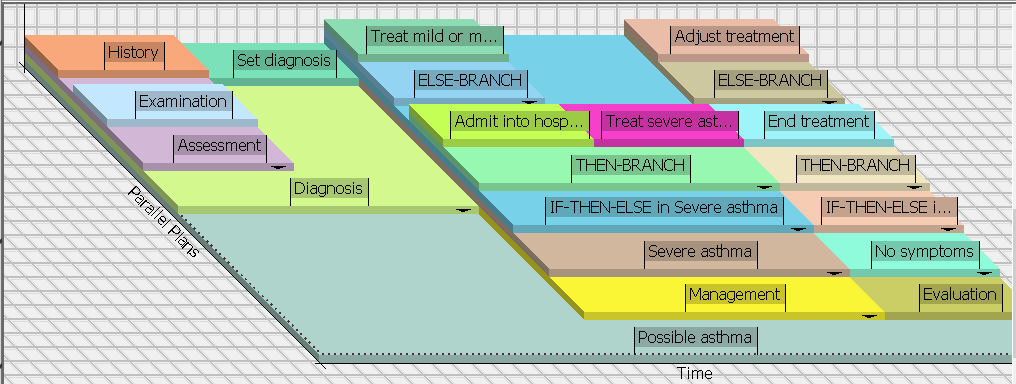
\includegraphics[scale=0.55]{AsbruPossibleAsthma}
	\end{figure}
	\item See the description of \textbf{DPF} in other parts of this thesis.
\end{itemize}
Studying PROforma, GLIF and Asbru we learn that there are several ways to approach the task of making computer interpretable guidelines. We can learn about challenges and see how they solved them. Dissemination, where one needs to regularly update the guidelines and make sure that the different computer systems use the updated versions, is such a topic. Dissemination is relevant for this project, as you want to make sure that every student trains for the most current guideline. You don't want them to memorize old and outdated content.

Our conclusion is that Asbru, GLIF and PROforma are rather large systems, putting a lot of emphasise on working in a hospital setting, communicating with other computer systems such as decision support on the electronic health record. With large computer systems, it is much more difficult to customize.

They also work on a higher abstraction level than the symptoms the clinician needs to look for when doing an examination for asthma. When training clinicians, we are very interested in modeling the details a clinician has to do during a clinical encounter. Asbru, GLIF and PROforma are more concerned with customizing the workflow for one or a sequence of treatments for a medical conditions. We want to use more general models which can be reused to represent several guidelines. With DPF we can create custom domain specific modelling languages.


\subsection{Designing alternatives}
The goal of the iteration is to decide what kind of application to build. What type of application can we best promote the CPGs, and encourage health personnel to use and learn them.

For this iteration it was quite critical to get background information on CPGs, how they are used in the hospital, how they are used by medical students today and how they work in different areas. For this we needed the results from the iterations about the focus group and studying similar products. We also had a medical domain expert in our project. Informal literature studies was also necessary.

A lot of different prototypes at lower and higher fidelities were made. Some were made initially at higher fidelity levels as a part of testing technology. Figure \ref{fig:ConseptualModel} was such a prototype to  test technology, as well as exploring how to organize and categorize CPGs. Figure \ref{fig:SimulationTool} was a prototype of a simulation tool, but also had the purpose of uncovering details of the paediatric possible asthma guideline \parencite{RepublicofKeny2016} when communicating with a medical domain expert. 

Figure \ref{fig:PrototypeInteractiveCPG} was also a prototype initially at higher fidelity as we tested SVG generation with JavaScript. The idea of the prototype was to display CPGs as interactive flow-chart. The vertices have a topic which can be clicked. By clicking, the vertex will either expand to show more detailed information or will redirect to a subguideline. The edges represent decisions and workflow. An idea was also to enter patient specific details such as gender, age and weight and possibly symptoms, and get the CPG customized for that patient.


 \begin{figure}[h!]
 	\caption {A design alternative, displaying the CPGs as interactive flow-charts. The edges represents the flow, while clicking vertices will display more information or redirect to subguideline. A suggestion was to fill in with patient and examination data, to get a customized CPG for a patient }
 	\label{fig:PrototypeInteractiveCPG}
 	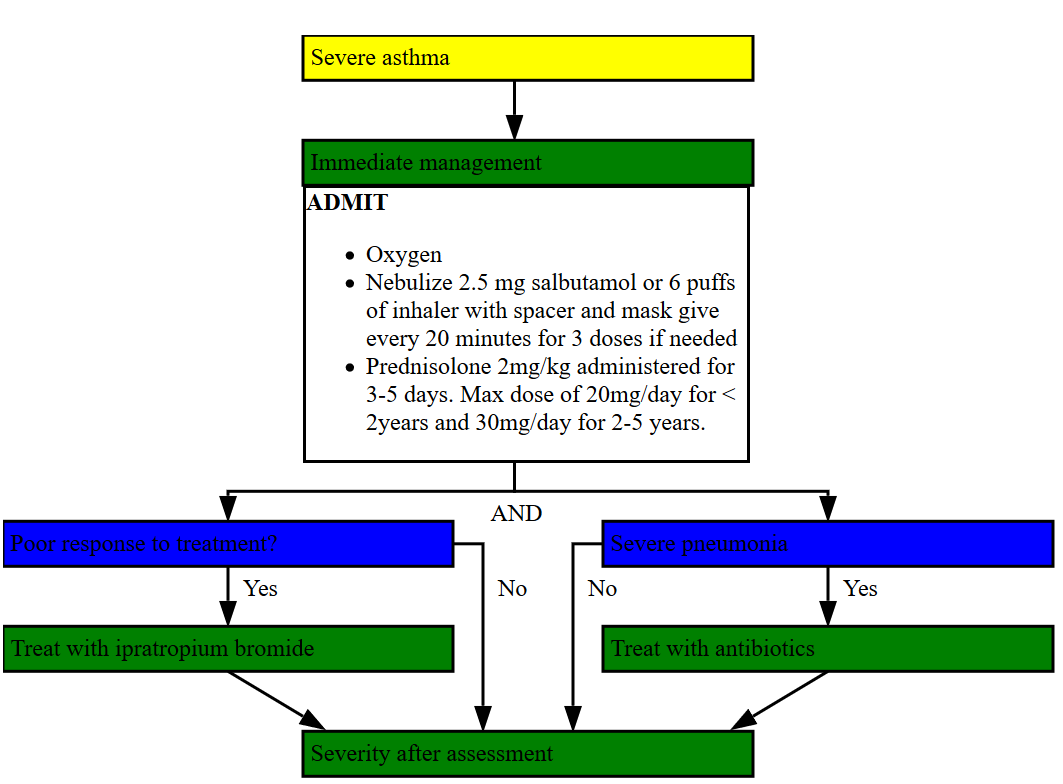
\includegraphics[scale=0.6]{PrototypeInteractiveCPG}
 \end{figure}

The prototype in figure \ref{fig:PrototypeGameCPG}, started as sketches with pen and paper. By going through several iterations of redesign, it reach the fidelity of figure \ref{fig:PrototypeGameCPG}. This was our first prototype where we presented the CPGs as a game. We got help from an external masters degree student in software engineering to make this prototype. The concept of the game is that you initially get presented with a list of tests you can do on the patient. By picking a test, you will immediately get presented with a test result. You can do more tests or proceed. In the next screen you will be presented with a list of treatment and advises, and you should pick the correct ones with the knowledge you acquired in the previous screen. In the last two screens, you will be presented with the answer keys. You will get points for choosing the correct treatments and advises. You will get points for picking the right tests, and you will get higher scores if you picked the tests in an optimal order.
\begin{figure}[h!]
	\caption {The first design alternative proposed as a game. The student tries to pick the right tests in the right order for that patient. As well as choosing the correct treatment and give the right advises to the patient. A high score for choosing the right treatment and advises, as well as correct tests in the right order. Medium score for right tests in the wrong order}
	\label{fig:PrototypeGameCPG}
	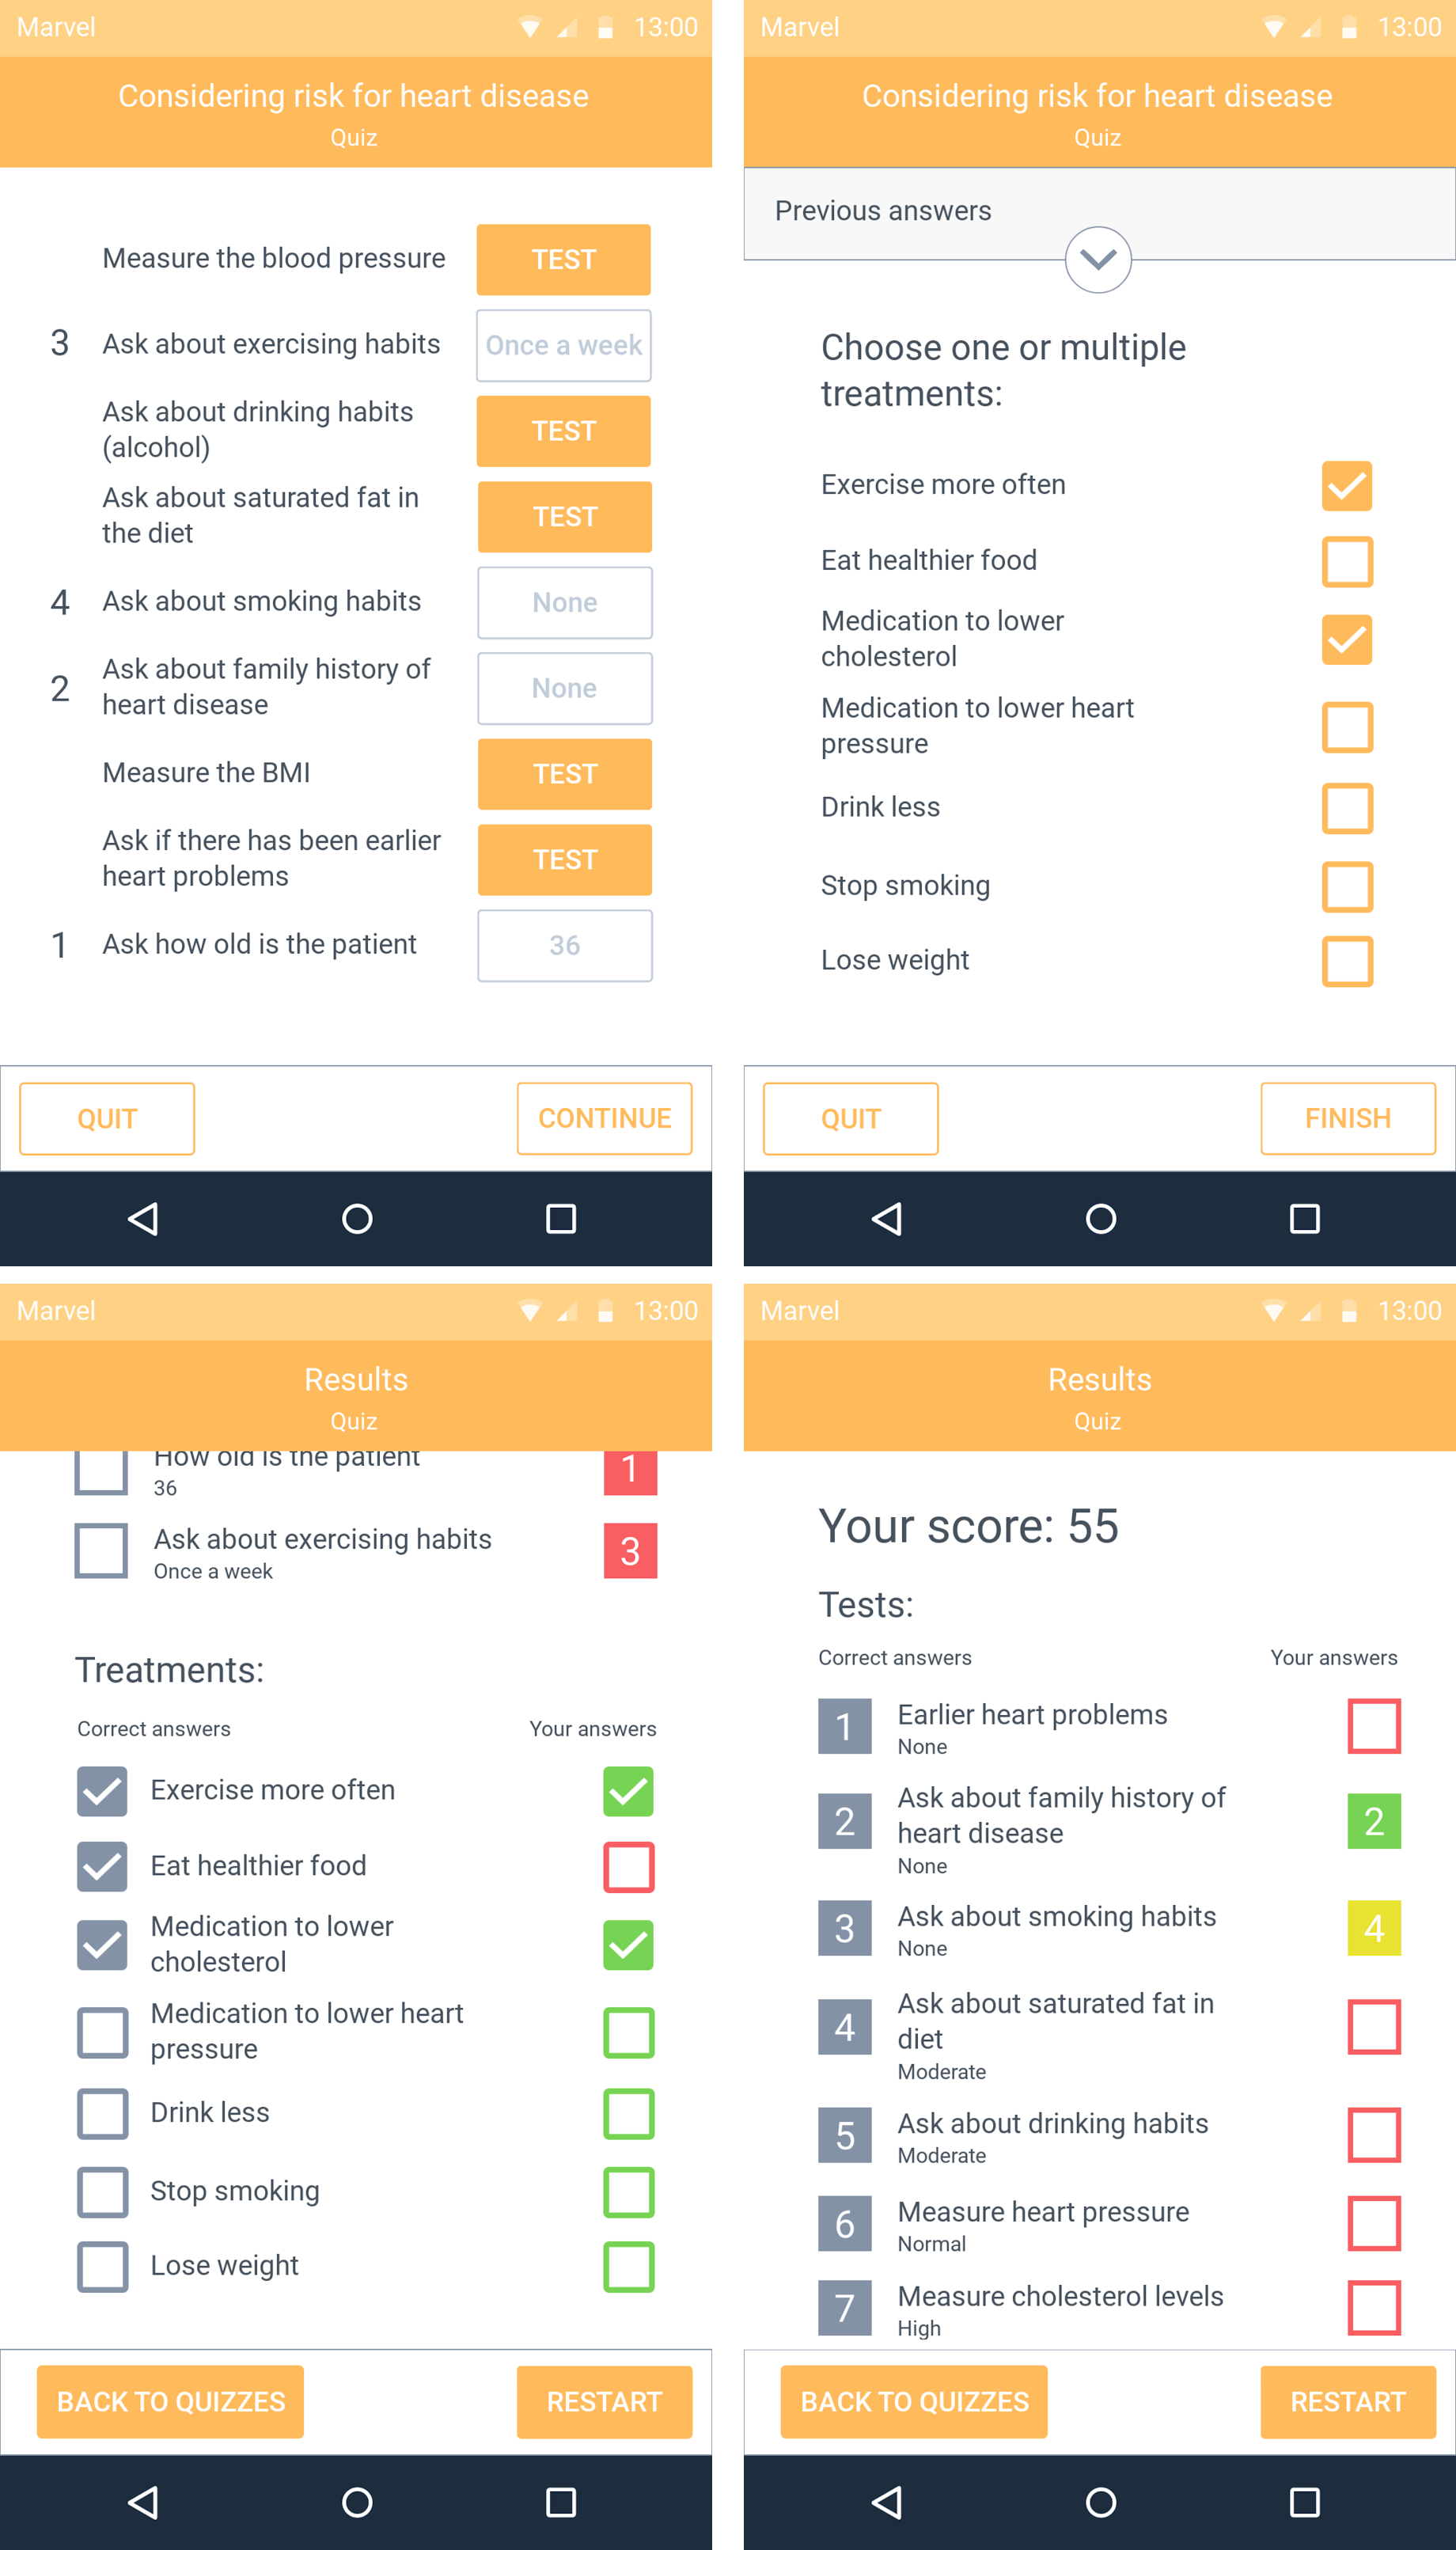
\includegraphics[scale=0.2]{PrototypeGameCPG}
\end{figure}

The design alternatives were evaluated with the project's supervisors and their master degree students. There was also separate evaluations with medical domain expert. The evaluation method was cognitive walkthroughs as well as discussions what is the best approach for promoting CPGs and encourage medical students to learn and use CPGs. The conclusion was to continue with game development. 


\subsection {Entity and workflow models}
The goal of the iteration was to model patients at different stages of the clinical encounter. The entity model should be able to represent patients in scenarios in quizzes with answer keys.

We based our models on the paediatric possible asthma guideline \parencite{RepublicofKeny2016}. The first step was to understand every symptom, medication, equipment used in the treatment and keywords such as "admit". Resources like \textcite{Disease2011} and \textcite{Johansen2018} were some of the resources used, but most importantly was an expert of domain. 

The developer made a prototype of his understanding of the CPG, which simulated a clinical encounter with a patient. See figure \ref{fig:SimulationTool}. The GLIF chart presented in figure \ref{fig:GLIFPossibleAsthma} was used as a base when making the simulation tool. The simulation would start with listing symptoms of asthma and the clinician would choose among the symptoms, redirecting to the treatment for severe, mild, moderate and no asthma. The simulation would continue with cycles of evaluating the given treatment, and the clinician needs to act accordingly to the evaluation for each cycle until the treatment can be ended. An expert of domain got the task of going through the entire simulations of use cases such as "a patient with severe asthma responds poorly to salbutamol treatment". The stimulation gave a thorough understanding of the guideline, emphasized details which would have been missed or details of the treatment which is left out of the guideline itself, such as differential diagnoses.

\begin{figure}[h!]
	\caption {Screenshots of the prototype used to simulate a clinical encounter with a domain expert}
	\label{fig:SimulationTool}
	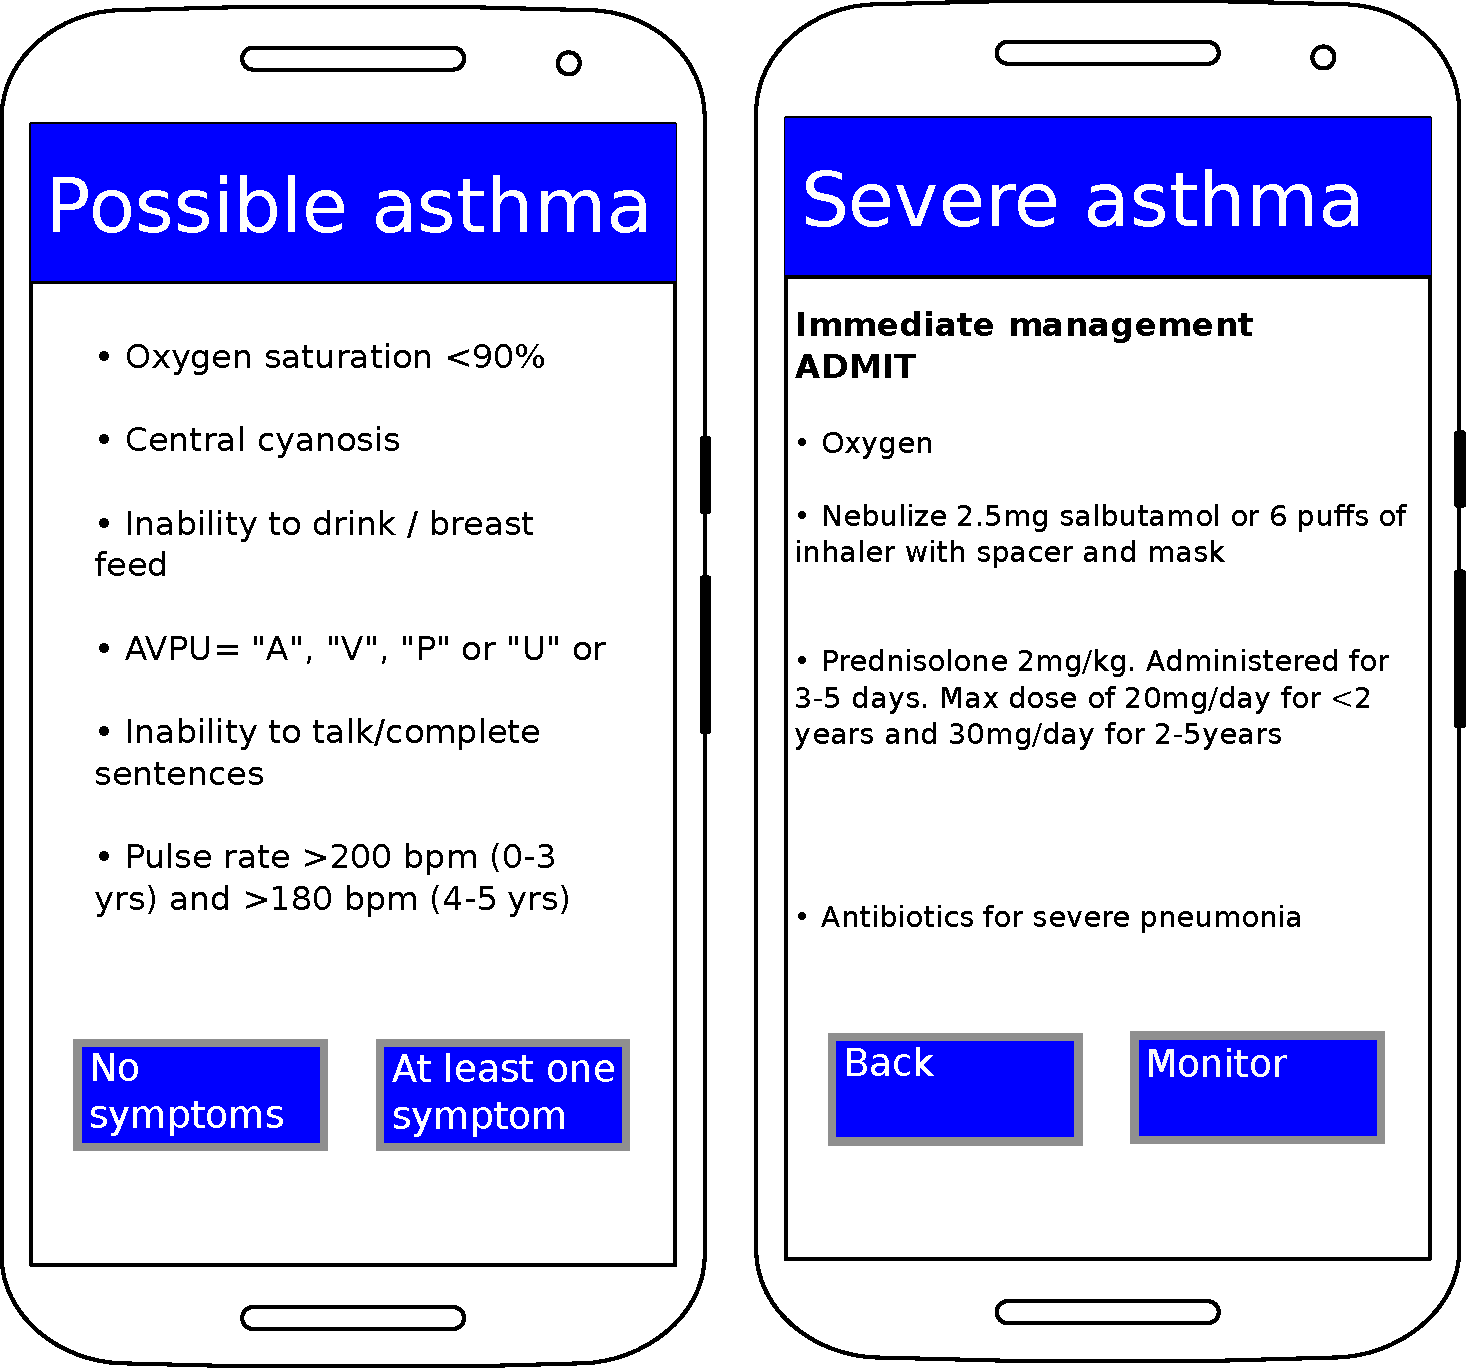
\includegraphics[scale=0.4]{SimulationTool}
\end{figure}

The guideline is also unclear at some points, where a discussion with a domain expert was needed. For example: wheeze + history of cough or difficulty breathing. When parentheses are not used, it is difficult to see if wheeze always needs to be  present, or if it is enough that cough alone is. It is also difficult to understand the effect and model the situation where the presence of a symptom at a certain age gives "increased likelihood" for asthma. In computer science the terms need to be very clear.

A domain expert in Model Driven Engineer and DPF was consulted for discussing problems such as inheritance, how to create good sentences from vertex values in the graph, as well as metamodelling and the use of constraints in DPF. In figure \ref{fig:BlackboardingDPF} there are two images from the whiteboard during the meeting. On the left we see a workflow and an instance below. The XOR is a constraint, which tells that we can choose one of the two  paths only. On te right we see the entity model, and a suggestion with vertices which make good textual presentation of graph values which can be used in texts. 
\begin{figure}[h!]
	\caption {Pictures of the whiteboard during a meeting with domain expert in MDE and DPF. To the left there are some discussion around workflow models. To the right is entity models with vertices which holds a textual representation of the parent vertex.   }
	\label{fig:BlackboardingDPF}
	\includegraphics[scale=0.16]{BlackboardingDPF}
\end{figure}

For evaluating the entity model, a domain expert in medicine made quizzes with factual questions as well as scenario based. By replacing patient related variables in the questions and scenarios, with tags pointing to variables in the entity model, we could see whether the model fulfilled the requirements of displaying good and valid sentences. The sentences were equally good and valid when using different instances of the entity model.

The workflow model got evaluated by making quiz scenarios, and by confirming that these scenarios covered the entire guideline.



 
\subsection{User experience}
The goal of the iteration is to facilitate the application for good user experiences.

First of all we need to clarify what a good user experience is. We are not going to dive in detail into figure \ref{fig:Hassenzahl}, but shortly explain the components he \textcite{Hassenzahl2006} defines.  
\begin{itemize}
	\item Beyond instrumental, has to do with other aspects than reaching a work related goal or solving a work related task. It has to do with attraction and feelings, such as attraction to a beautiful design, the feeling of trust, quality and reliability or the user feels motivated through personal growth and increase of knowledge and skills \parencite{Hassenzahl2006}. 
	\item Emotion and effect, has to do with how the users feel when interacting with the application. Typically we want the user to feel joy and excitement, and damper or prevent feelings such as frustration, anger and disappointment \parencite{Hassenzahl2006}. Typically the user feels satisfaction when completed a work task, or frustrated when the work task takes a long time to complete. 
	\item The experiential emphasizes that the experience is strongly related to the situation it is used in and at which time. \parencite{Hassenzahl2006}. As an example the user experience of listening to your favourite music artist in the car on the way to work, is different from being at a concert in the weekend with the same music artist.
\end{itemize}
\begin{figure}[h!]
	\caption {User experience copied from \textcite{Hassenzahl2006}}
	\label{fig:Hassenzahl}
	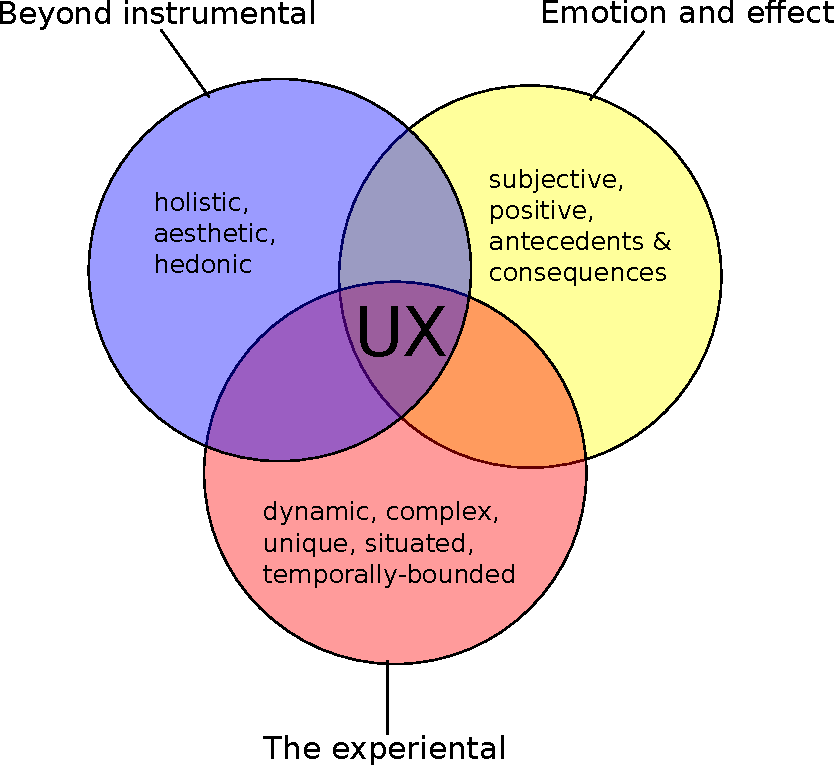
\includegraphics[scale=0.66]{Hassenzahl}
\end{figure}

For the beyond instrumental, we used several iterations to make a pretty user interface to make the application desirable. As this is an educational tool, it is important that the user feels his skills and knowledge grow, so the visualization of progress was quite important. Both that the user advances in levels, but also that we visualize the progress during a level, where the user stretches to slowly meet the requirement of the next level.

For emotion and effect, we should trigger joyful emotions, such as emphasizing when the user answers correctly and progresses. We should use kind and encouraging wording when the user makes an attempt and doesn't get the right answer or doesn't progress to the next level. The interactions should be clear such that the user easily can fulfil his goals and doesn't make mistakes. Keep system errors to a minimal. In our evaluations we could probably more encouraging to the user when he gives a wrong answer.

The experiential use is a bit hard to adapt to. We have been thinking that this is a mobile app, often played when the user is bored and can be situated anywhere. Perhaps on the bus to the university, or waiting for his friends in the cafeteria. The buttons should be large, large font size and small amounts of text on the screen, clear instructions and that the user doesn't have to remember information from previous screens are good guidelines in an environment which can be distracting. This is also according to Jakob Nielsen and Rolf Molich heuristics about user design. "Minimize the User’s Memory Load" and  "Simple and Natural Dialogue" \parencite{Molich1990}.

The user experience was evaluated using cognitive walkthroughs with the supervisors and their master degree students. We had a cognitive walkthrough with a domain expert in interaction design and gamification, followed by discussion and tips for further improvement. Some of the feedbacks were "wrong" in red colour may be too harsh, as well as a penalty of negative points even though the penalty is not displayed. A user should be able to get a higher score than just the requirement for the next level.

We used usability tests in controlled environment, where friends, family, fellow students and domain expert in medicine were asked to start the application and play a full quiz. Notes were taken at points where the user would do  mistakes, get confused or do a mistake. Typically the user would become very confused when seeing the screen with the learning map, displaying which levels have been completed, which we are currently playing and the locked levels. The user would typically try to click on completed or current levels. We also noticed that the students wouldn't revise a wrong answer, just continue to the next question.


\subsection{Game Engine and Content Flow}
The goal of the iteration is to have a playable game, which produces questions, answering elements, rewards, several difficulty levels and the flow of the game content.

This iteration draws upon the work which have been produced in other iterations. Producing the content quiz questions was done together with a domain expert in medicine. As part of the Game Engine, we developed a template system, where we replace variables in the question content with tags which refers to vertices in the entity graphs. We can evaluate to see that the game engine produces sensible questions and answer elements.

The ideas of difficulty levels and the flow of the game content were discussed in the workshop section. This iteration was about implementing and testing these parts of the Game Engine.

The scoringsystem was developed, where we give scores per question element in the workflow model.  A penalty system was introduced, such that a student with many attempts on each question doesn't get the same total score as a student which answered every question correctly on the first try.

The evaluations of the iteration were done as part of the user experience iteration. Mainly cognitive walkthroughs with domain experts, but also usability testing in controlled environment with non-experts.




\subsection{Focus group}

\subsection{Workshop}

\chapter{Architecture Overview}
\section{Architecture of the whole system}
The architecture of the system is shown in figure \ref{fig:Architecture}. The system in it's whole is running on the student's phone. The main components are the presentation layer and the game engine, where the purpose has been to make the game engine very generic and loosely coupled from the presentation layer. By replacing the presentation layer, the Game Engine can be implemented in a web application or using Google Assistant which uses voice to interact. 

We'll briefly dicuss the the architecture of the system in the following subsections, before we'll give a more thorough expalantion.

\begin{figure}[h!]
	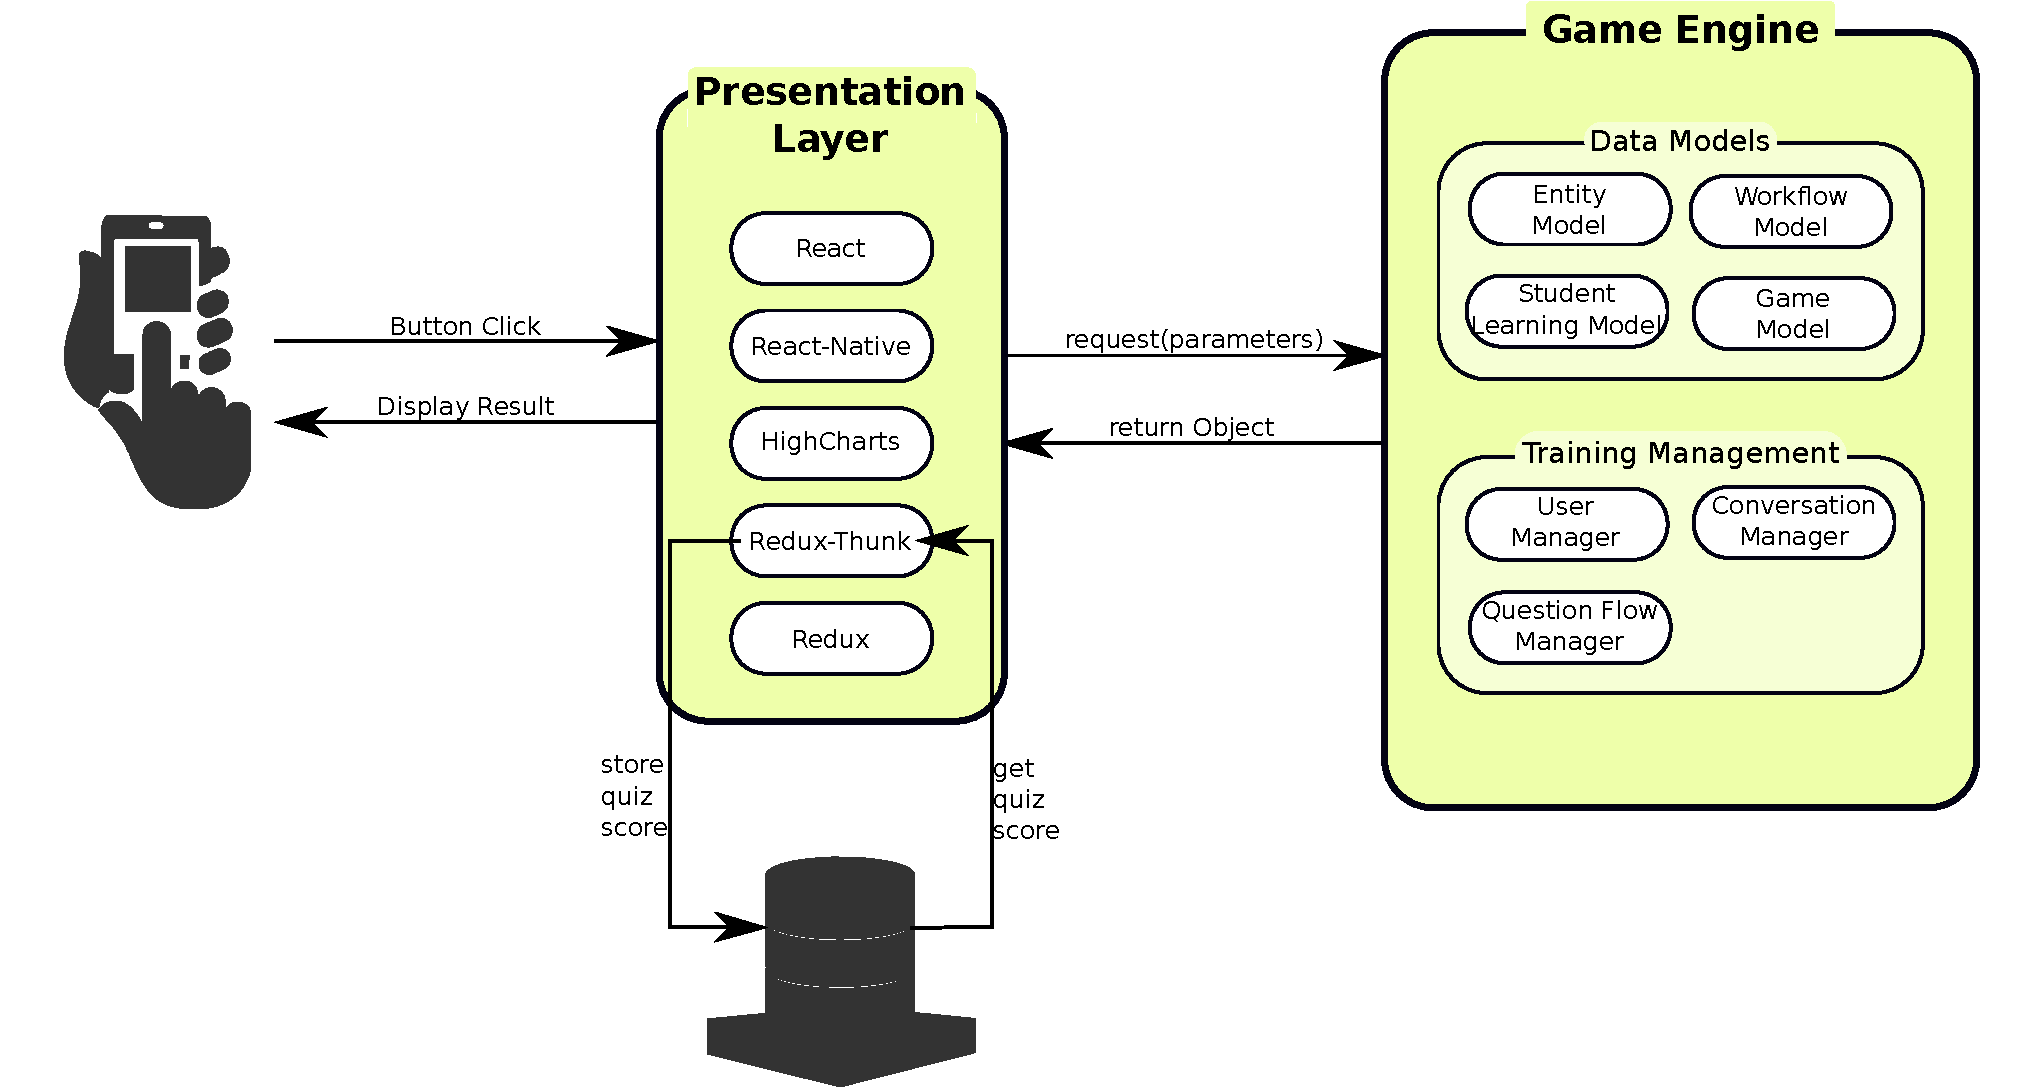
\includegraphics[scale=0.4]{Architecture}
	\caption {Overview of the system architecture}
	\label{fig:Architecture}
\end{figure}

\subsection{Presentation Layer}
The presentation layer is what the user sees and interacts with when using the application. React Native \parencite{ReactNative} is a JavaScript framework, used to build cross platform mobile applications for Android, iPhone and UWP. It is based on React \parencite{React}, where it uses React components to build user interfaces for mobile applications. 

For managing the state of the application, we use another JavaScript framework, Redux \parencite{Redux}. It is sort of a repository of functions and variables. When the student clicks on a button in the application, it will trigger a function in the Redux repository. The function can send a request to the Game Engine or do some calculations in its own. Then update a variable in the repository which is connected to a variable in the React Component, and the result is shown on the student's phone.

As the Redux repository is synchronous, we need the framework Redux-Thunk \parencite{ReduxJS-thunk} to make asynchronous calls. A student's scores for a quiz is stored in the database on the student's phone. The game engine uses the scores to find questions at the right difficulty level for the student. As database calls are asynchronous, we need Redux-Thunk to make functions which can do asynchronous communication between Redux and the database. 

HighCharts \parencite{Highsoft} is a JavaScript framework used for making interactive charts. We use it to visualizing how well the user performed, and how far he is from advancing to more difficult questions.  

\subsection{Game Engine} 
The game engine initializes the quiz, controls the training flow, produces questions with answering elements and keeps track of the user's performance. 

The data models are used to hold information and represent a domain of concepts. The entity model represents a patient at different stages under a clinical encounter. The workflow model describes different processes at a clinical encounter. The game model holds relevant game information such as questions at different categories and difficulty levels, distractions, points and penalties for each distraction, answer keys and answer key explanations. The student learning model keeps track of the student's scores at different quizzes.

The managers are conceptual, used to better describe the responsibilities of the game engine in this section. 

The question flow manager adapts the questions to the knowledge level of the student, and is flexible such that the student can choose his own path through the completion of each difficulty level. 

The conversation manager puts the questions with belonging answer elements in a sequence such that they fit to a scenario, using the workflow model. The conversation manager produces questions and answer keys from a template, in which the entity model is used to fill in data for the place holders in the template.

The user manager keeps track of the user's skill, based on the performance on previous quizzes. It holds the scores for the current quiz, and it measures the user's progression. 

\section{Summary}
We have proposed an architecture of the systems. The mobile application logic is in a separate loosely coupled presentation layer, sending requests to a platform independent game engine. 

For the game engine, we have separated the concerns. We have four data models and three conceptual training managers, and given a brief description on all of them. The game models and the conceptual training managers will be thoroughly discussed in the two following chapters.

\chapter{Datamodels}
\section{Extracting knowledge from the clinical  practice guidelines}

For this project and according to the research questions, we will be using four models.
\begin{enumerate}
	\item An \textbf{entity model}, which will be a model of the domain concepts. The patient, the different methods for discovering and measuring symptoms. The patient's medical condition and the procedures done to manage the patient's medical condition.
	\item A \textbf{workflow model}, which describes the different processes in a clinical encounter. This will be the flow of the guideline itself at an abstract level.
	\item A \textbf{game model} which will contain the game elements, as well as the order in which the student will learn parts of the guideline. By game elements we mean the questions, distractions, answer keys, answer key explanations, rewards and penalties for the different answer alternatives, as well ass passing conditions for the different difficulty levels.
	\item A \textbf{student's learning model} for monitoring the student's learning progression.
\end{enumerate}

Models are good for sketches, where we can easily discuss with team members, domain experts and possibly stakeholders. The models can hold a detailed specification of the system, as well as we can use models instead of code to develop the system \parencite{Brambilla2017}.

For this project communication is very important, as the developer needs to understand and be able to model the clinical practice guideline and the clinical encounter at a very high detail. The domain expert in medicine needs to be able to verify that the model is correct.

\section{Extracting knowledge from the clinical  practice guidelines}

\section{MDE and meta modelling}
We will be using a Model Driven Engineering (MDE) approach, mainly for the entity and workflow models. In MDE models serves as the key artefacts that drive the development process \parencite{RodriguesdaSilva2015}. A model in this case is an abstraction of a system under study. It is usually a partly and simplified version of the system, where we often need multiple models to better represent and understand it \parencite{RodriguesdaSilva2015}. A domain model is the conceptual model of a field or expertise that we are examining to solve a problem \parencite{Brambilla2017}.

A metamodel is a model where one define the modelling concepts that will be used to represent the system in.

A metamodel is a further abstraction of a model, which highlights properties of the model \parencite{Brambilla2017}. In figure \ref{fig:Metamodelling} we see that moving up through the levels is an abstraction of the previous model. While moving downward, we are making instantiations of the previous metamodels. With metamodels we can define new languages, as well as defining new properties or features of the available information \parencite{Brambilla2017}. This allows us to make Domain Specific Languages (DSL), which is designes specifically for a specific domain and context \parencite{Brambilla2017}\parencite{RodriguesdaSilva2015}. By using DSLs, we can develop more expressive models, which can enhance communication with or be used by domain experts. 

\begin{figure}[h!]
	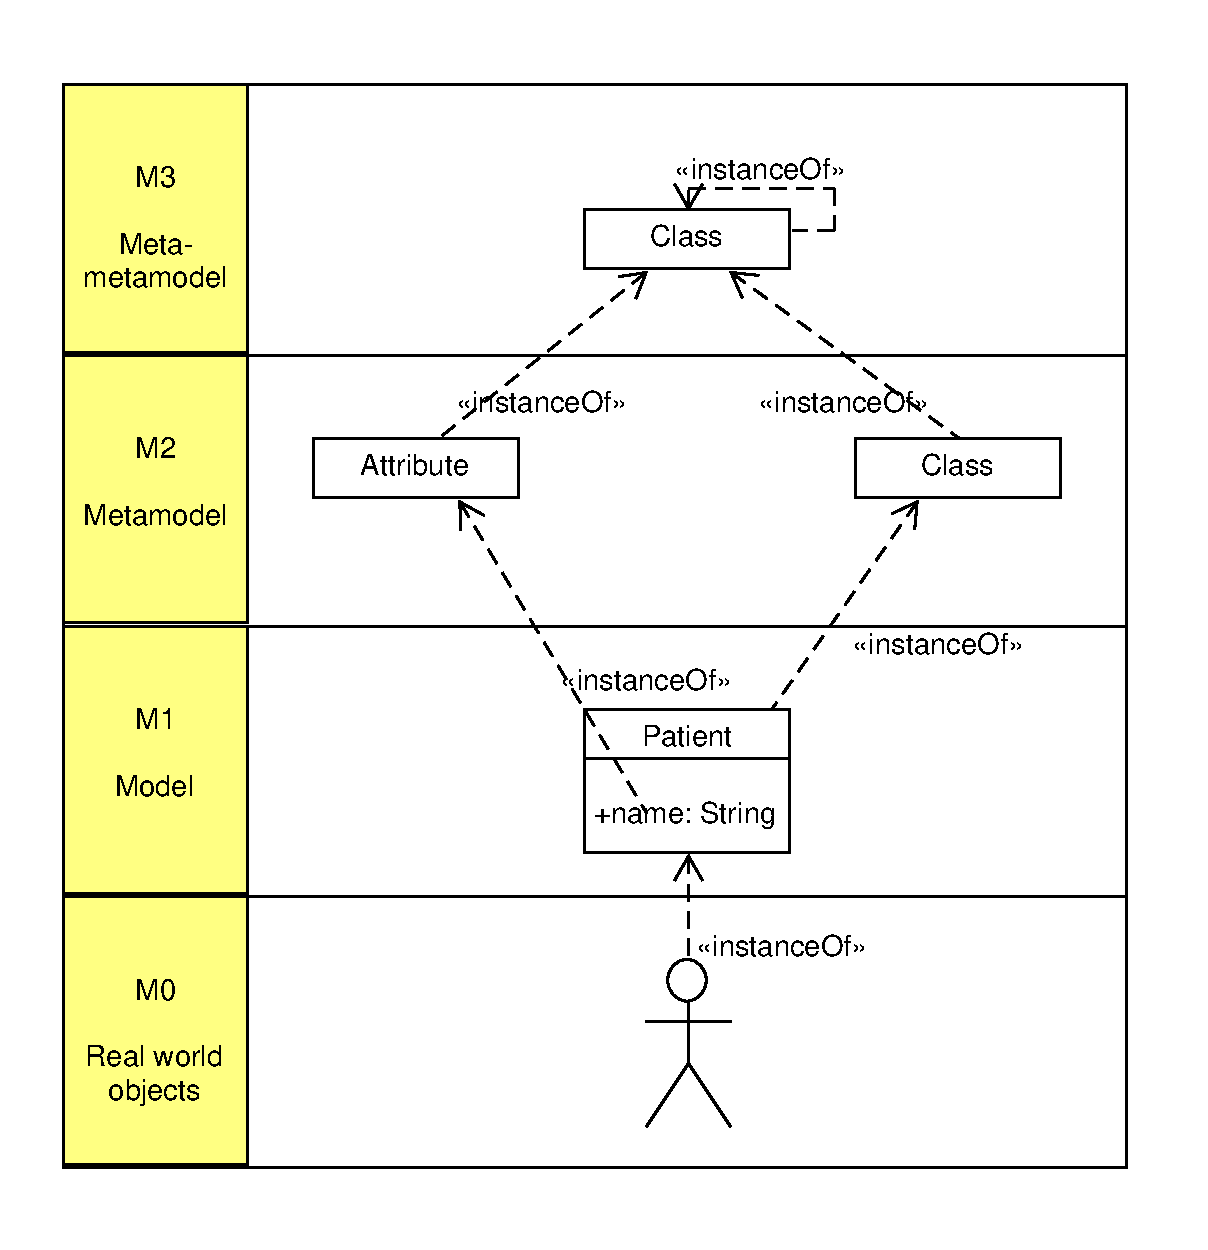
\includegraphics[scale=0.5]{Metamodelling}
	\caption{Metamodeling from a meta-metamodel to a real world object. Derived from \parencite{Brambilla2017}}
	\label{fig:Metamodelling}
\end{figure}

% Say something about how the graph is implemented and a reference to the book.
\section{DPF}
For the enitity- and workflow models, we use a formal diagrammatic approach to model driven engineering, which is called Diagram Predicate Framework (PDF). In software engineering, diagrams are data structures based on graphs. A graph is a collection of vertices, which may be connected by edges.

A definition for DPF is given by \textcite{Rutle2010}: "in DPF, models are represented by a diagrammatic specification \(\mathfrak{S} = ({\mathcal{S}}, C^{\mathfrak{S}} : \Sigma)\). It consists of a graph \(\mathcal{S}\) and set of constraints \(C^{\mathfrak{S}}\) specified by a signature constraint $\Sigma$ ". To simplify the definition to how it is used in this thesis, the models and initiations are represented and implemented using graphs and a set of constraints. The following sections will discuss these graphs in detail.

Why do we use DPF and not a system such as fHIR? DPF is an abstract modelling formalism that could be used to model different aspects of the system. HL7 fHIR is a domain specific language to represent (and share) resources (i.e. domain concepts) in health care. 
\section{Entity model}
\textcolor{purple}{TODO Yngve: Explain the main entities in the entity model here}
We will now present the entity model by showing an excerpt, hiding away the details. This will let us easier focus on the concepts and the flow, as the model itself is quite large and complex. See figure \ref{fig:EntityGraphExcerpt}

The entity graph stores information about a specific patient at a certain point of time in the clinical encounter. The patient comes to the emergency clinic. He has some symptoms which the clinician needs to uncover, by doing examinations and asking questions about the patients conditions. What the patient or caregiver tells is modelled as history, while quick examinations such as listening to the chest, looking at the skin, count the number of breaths per minute are modelled in the examination vertex. In some cases the clinician wants to run medical tests which require more time and resources, such as MRI scan, spirometry or blood tests. These tests are modelled as investigations.

Based on the the symptoms collected in history, examination and investigation, the clinician will set a diagnosis. The procedures for what to do with a patient with a given diagnosis is modelled under management. Hospitalization is to change the patients status to outpatient, or inpatient if he is admitted into the hospital. He might need some medication or be given advise for how he should deal with his condition the in every day life. Here the model can be expanded with routines found in other guidelines, we have identified surgery as an example. 

\begin{figure}[h!]
	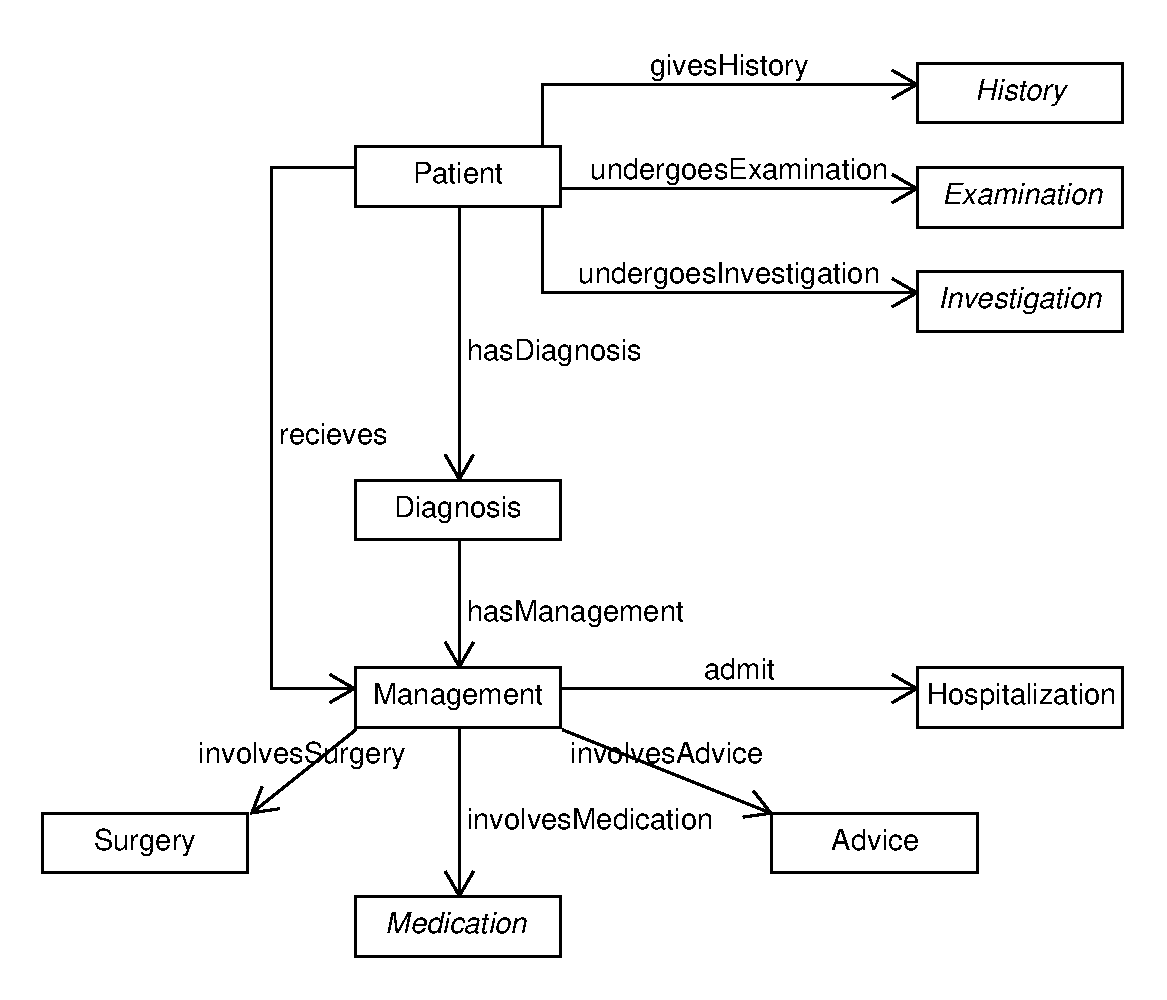
\includegraphics[scale=0.6]{EntityGraphExcerpt}
	\caption {An excerpt of the entity graph. Entity graph represents a patient at a certain point in the clinical encounter}
	\label{fig:EntityGraphExcerpt}
\end{figure}

In figure \ref{fig:EntityGraphPatientDiagnosis} we have expanded the Patient and Diagnosis vertices to reveal more details. PatientName and Gender, identifies the patient with a name and gender. These attributes are important when presenting a patient and his condition in a narrative or scenario. By using a name, it is easier for the reader to see that this is the same patient in different stages of the clinical encounter.

A diagnosis has a name. In the paediatric possible asthma guideline \parencite{RepublicofKeny2016}, the diagnosis has a severity. A lot of medical conditions doesn't have a severity, or they are classified in another way. Here we add multiplicity to the edge which specifies this requirement. 

\begin{figure}[h!]
	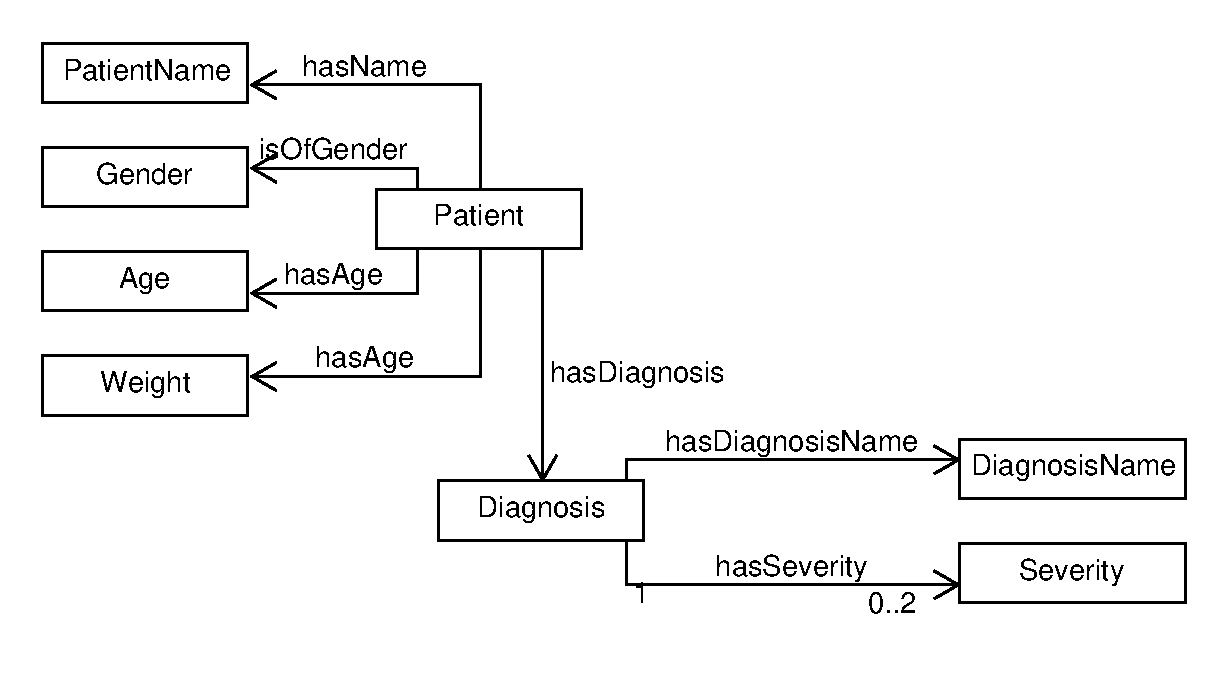
\includegraphics[scale=0.6]{EntityGraphPatientDiagnosis}
	\caption {Showing the details of the Patient and Diagnosis vertices of the entity graph}
	\label{fig:EntityGraphPatientDiagnosis}
\end{figure}

In figure \ref{fig:EntityGraphHistory} we have shown our implementation of the History vertex from figure \ref{fig:EntityGraphExcerpt}. History is what the patient or the caregiver tells about the patient's condition. In the paediatric possible asthma guideline \parencite{RepublicofKeny2016} we have identified three symptoms which the clinician can ask the patient or the caregiver about. Here we introduce inheritance, where the specific symptoms inherits the examination vertex. Each symptom the patient or caregiver tell about, will have a measurement. In this specific case, all the history symptoms are boolean. Either they have the symptom or they don't. The symptom values inherits from a Measurement vertex.

\begin{figure}[h!]
	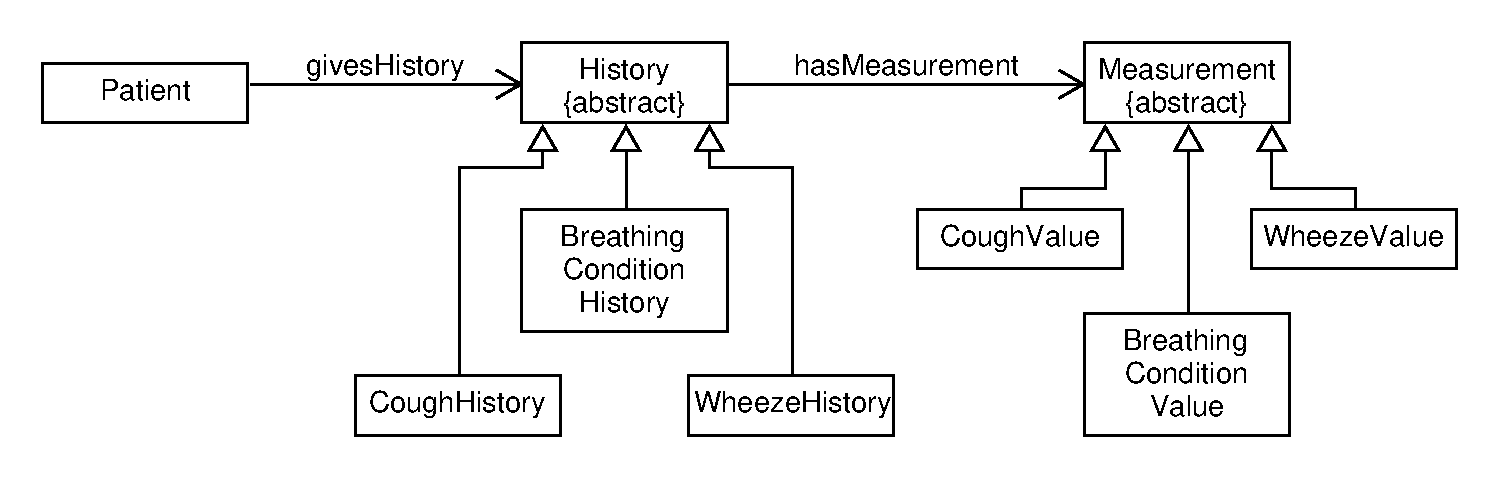
\includegraphics[scale=0.5]{EntityGraphHistory}
	\caption {Showing the implementation of History in the entity graph. What the patient or caregiver tell about the patient's condition}
		\label{fig:EntityGraphHistory}
\end{figure}

For Examination we follow the same principles as History. We implement it by letting each symptom inherit an Examination vertex. Each symptom has value which inherits from a Measurement vertex. In figure \ref{fig:EntityGraphExamination} we have shown the inheritances for each vertex with one arrow and a box. This is of practical reasons when drawing, as there are so many symptoms and it will be confusing to draw an arrow for each of them. Here the values which are stored are a bit more mixed than for History. Consciousness is measured using an AVPU scale, where A is the patient is Alert, V is Verbal, P is responding to pain and U unconscious. These are enumerates, where we store either A, V, P or U. Pulse Rate, Respiratory Rate, Oxygen Saturation are all numerical values. The other symptoms are registered as boolean values. Keep in mind that Jaundice is really not a part of the paediatric possible asthma guideline \parencite{RepublicofKeny2016}. It is included as part of the antibiotic treatment.


The implementation of Investigation would be just as we did with History and Examination. For asthma they use a lab test called spirometry, but it is not included in the paediatric possible asthma guideline \parencite{RepublicofKeny2016}, so we don't include it in our model

\begin{figure}[h!]
	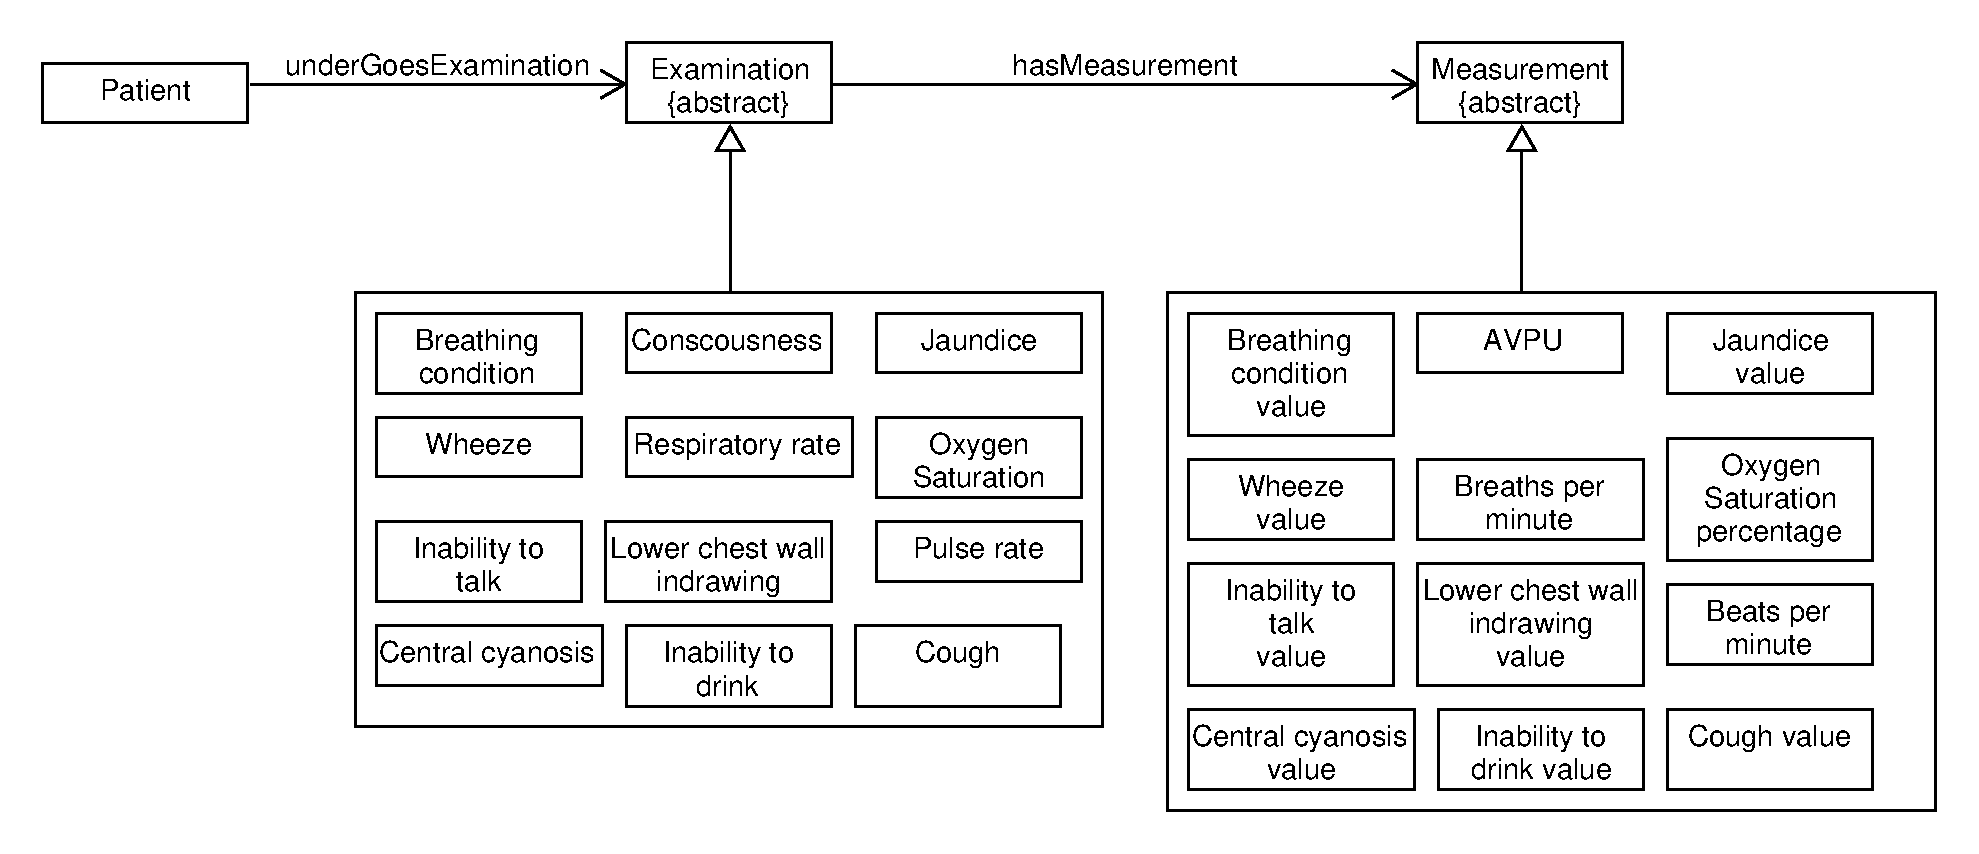
\includegraphics[scale=0.4]{EntityGraphExamination}
	\caption {Showing the implementation of Examination in the entity graph. What symptoms the clinician can observe the patient has}
	\label{fig:EntityGraphExamination}
\end{figure}

In the paediatric possible asthma guideline \parencite{RepublicofKeny2016}, there are used five medications to treat the patient, as well as antibiotics which is a class of medications. We will talk about each medicine in the model as there are some details which needs to be clarified. See figure \ref{fig:EntityGraphMedication}.


\begin{itemize}
	\item \textbf{Oxygen} is a medication, which is given to patient which doesn't get enough oxygen by breathing. In asthma this happens because of the airways are tightened. The paediatric possible asthma guideline \parencite{RepublicofKeny2016} doesn't specify how the oxygen should be administered, but the paediatric guidelines contain a guideline for prescribing oxygen\parencite{RepublicofKeny2016}. We have decided to model a part of the prescribing oxygen guideline, to be able to ask simple control questions to verify that the student still remembers how to administer it. Oxygen has a route, which is inhaled. The method is oxygen face mask with reservoir bag. The rate will be given in litres per minute. The duration of the treatment will be until the oxygen saturation is at a high enough level.
	
	\item For \textbf{antibiotics}, the CPG says the antibiotic should be given according to the paediatric pneumonia guideline \parencite{RepublicofKeny2016}. We have decided to include the antibiotic treatment in detail in the model, but we have also kept Antibiotic as a medication, such that we later can ask a question where we don't go in more detail than just antibiotic, which is the detail level of paediatric possible asthma guideline \parencite{RepublicofKeny2016}. The antibiotic treatment consists of two medications gentamicin and penicillin. Gentamicin and penicillin are given as an injection either intramuscularly or intravenously, which is modelled as Route and Method. The rate is given by iu per kg, mg per kg, per 6hours or per 24 hours. If the patient has jaundice, he shouldn't be given penicillin. How much penicillin and gentamicin will be given according to the patient's weight.
	
	\item \textbf{Prednisolone} is a steroid used to calm and prevent inflammation in the airways. The clinician will administer a dosage calculated by the patient's weight. There is a max dosage per day, and the age will determine how high that max dosage is. The rate is given in mg per day. The duration is 3-5 days. The route is oral and the form is tablet. In situations where prednisolone needs to be given more than 5 days, it will be administered with the route inhaled and form inhaler.
	
	\item \textbf{Corticosteroid} is another steroid, which is given to in scenarios of recurrence asthma symptoms. The CPG specifies that corticosteroid should be inhaled. This is represented in the model by the Route vertex. The method the which will be used to inhale corticosteroid is represented by the Form-vertex. The Form is MDI with spacer, preferably with spacer with face mask. 
	
	\item \textbf{Salbutamol} is inhaled to open the airways of an asthma patient. The Rate vertex tells at which rate the patient should be taking salbutamol. Asthma patient is given salbutamol at a rate of 2.5mg per 20 minutes if nebulized, or 6 puffs per 20 minute if the inhaler is used. The Duration is up to one hour or three doses if needed. The method is inhaled and the form is either nebulizer or inhaler.
	
	\item \textbf{Ipratropium bromide} is modelled much like salbutamol with a Rate and a Duration. The rate is given in mcg every 20 minutes for a duration of one hour if needed. The route is inhaled and the form is inhaler.
\end{itemize}

 We have kept the Dosage vertex, while it is not in use. It can be used to represent the total amount of a specific medication given to the patient during this treatment.
 

\begin{figure}[h!]
	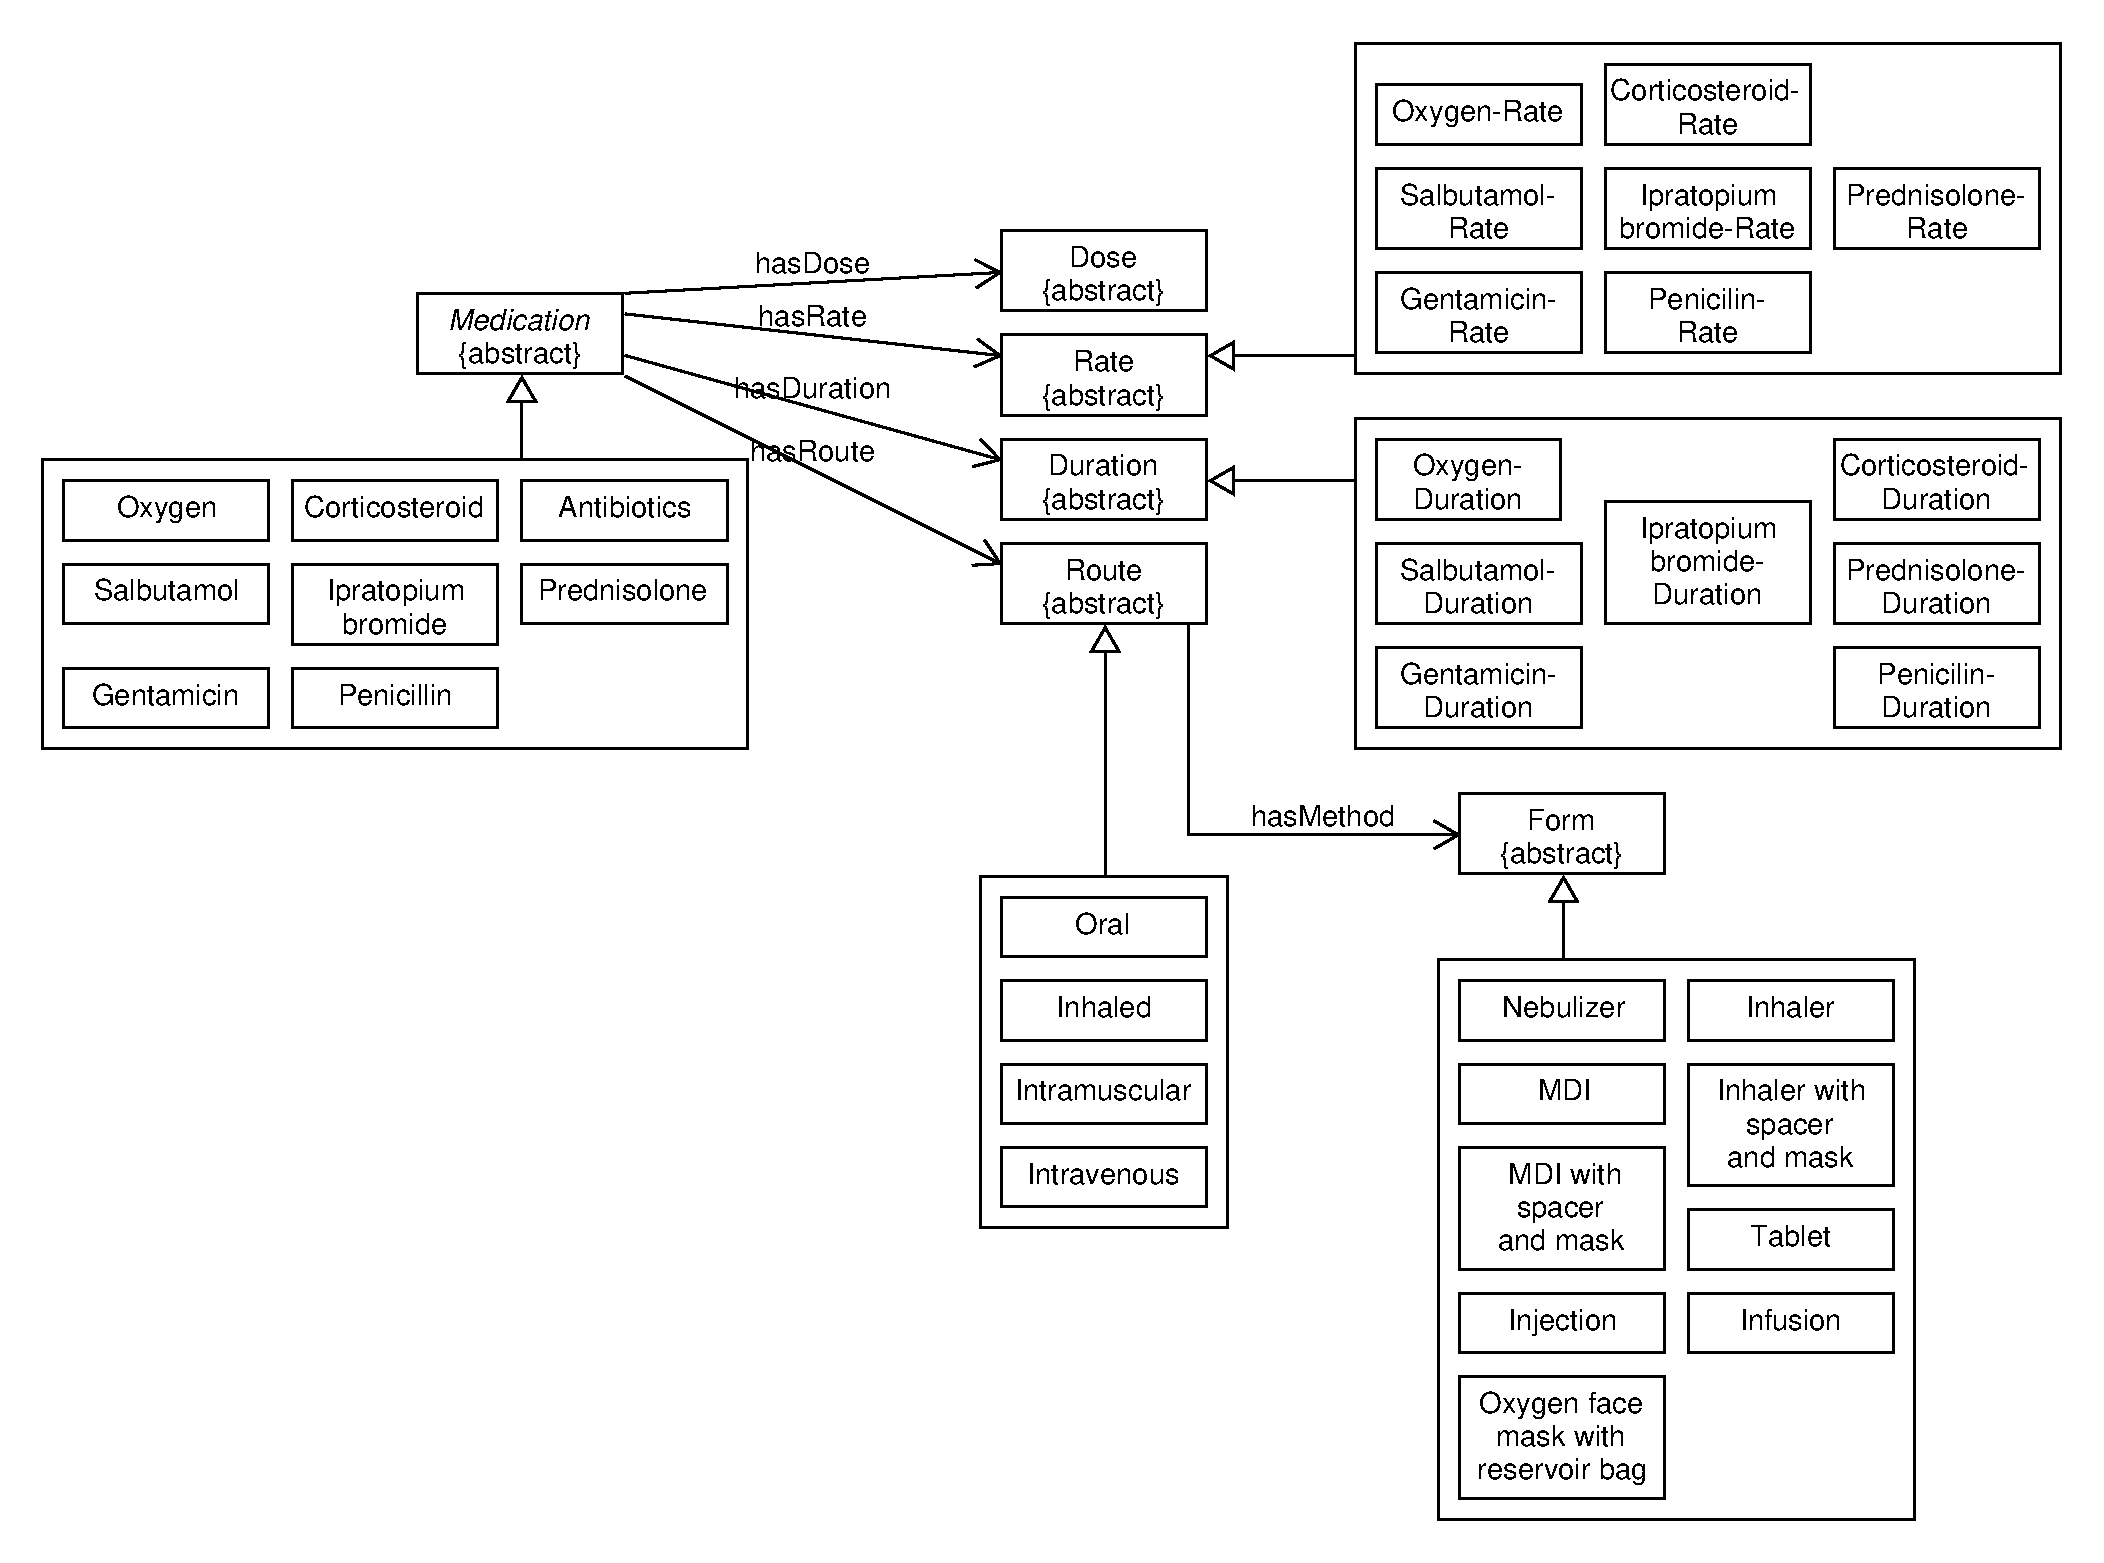
\includegraphics[scale=0.38]{EntityGraphMedication}
	\caption {Showing the implementation of Medication in the entity graph. How to administer a medication to patient}
	\label{fig:EntityGraphMedication}
\end{figure}

 Another detail must be clarified when implementing instances of the medications. The route must be given names which can be uniquely identified for each medication. An example is Ipratopium Bromide and Salbutamol which both uses the Route Inhaled. Ipratopium Bromide uses only the inhaler, while Salbutamol can be given using the nebulizer. If Ipratopium Bromide is sharing the same Inhaled vertex as Salbutamol during instantiation, it will look like Ipratopum Bromide can be nebulized. By creating a new instantiation of Route per medication, and uniquely identify them by name Inhaled1, Inhaled2 or InhaledSalbutamol, InhaledIpratopium, we avoid this problem. Now we can connect Salbutamol with Inhaled1 and have edges to Form Inhaler and Nebulizer. Ipratopium Bromide has an edge to Inhaled2, which has an edge to Inhaler. Then we have an instantiation where Ipratopium Bromide can only be inhaled using the Inhaler. See figure \ref{fig:RouteMethodProblem}.


\begin{figure}[h!]
	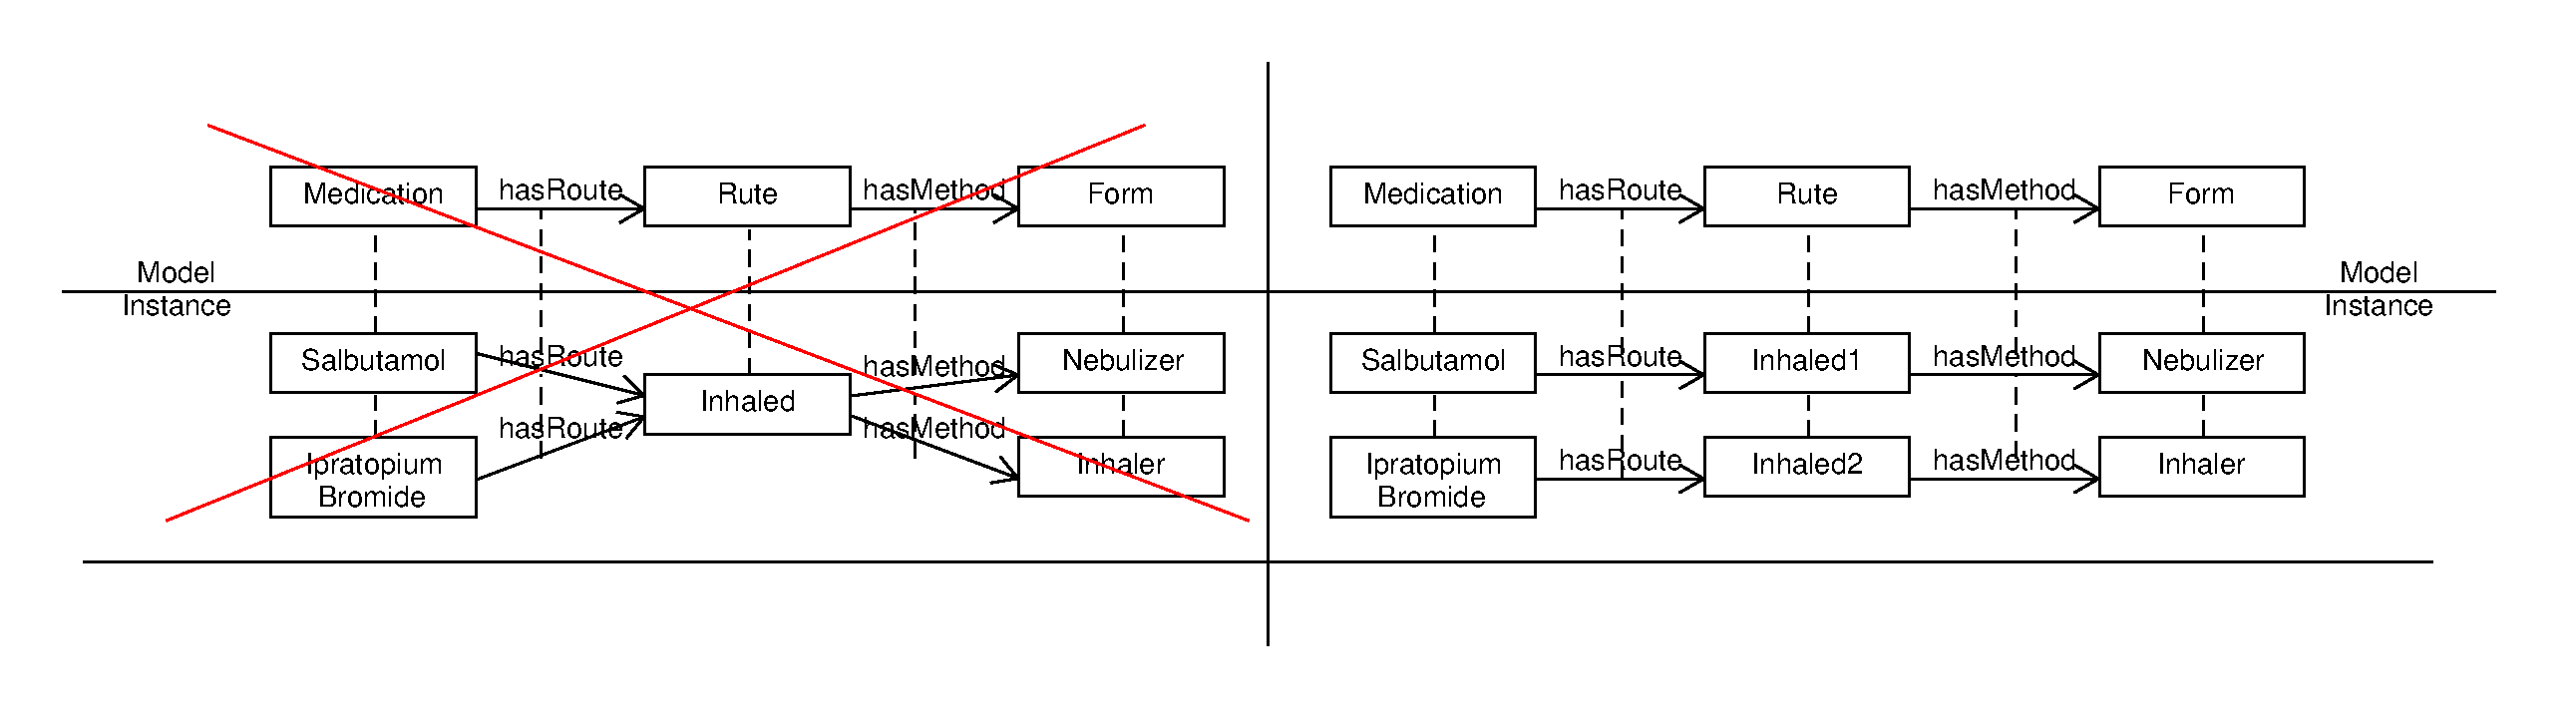
\includegraphics[scale=0.3]{RouteMethodProblem}
	\caption {To the left we don't know which medication has been inhaled using the nebulizer or inhaler. To the right we have specified this in the instantiation, by using two Inhaled-vertices and uniquely identifying them by giving them different names}
		\label{fig:RouteMethodProblem}
\end{figure}

\subsection{Generic entity model}
In the previous section, we had the focus on developing a specific entity model for the paediatric guideline of possible asthma \parencite{RepublicofKeny2016}. In fact by introducing inheritance, we actually made a specific and a generic model. In the model, we use the keyword \{abstract\} to note an abstracted vertex. The inheriting vertices become the specifications of the abstract vertex. 

In figure \ref{fig:GeneralEntityGraph} we have showed the the generic model. It only shows the abstracted vertices and not the specifications. A specific entity model for a specific guideline, will show both the abstractions and the specifications of them. The specifications need to be adapted for that specific guideline, and can not use the same as for paediatric guideline of possible asthma \parencite{RepublicofKeny2016}.

\begin{figure}[h!]
	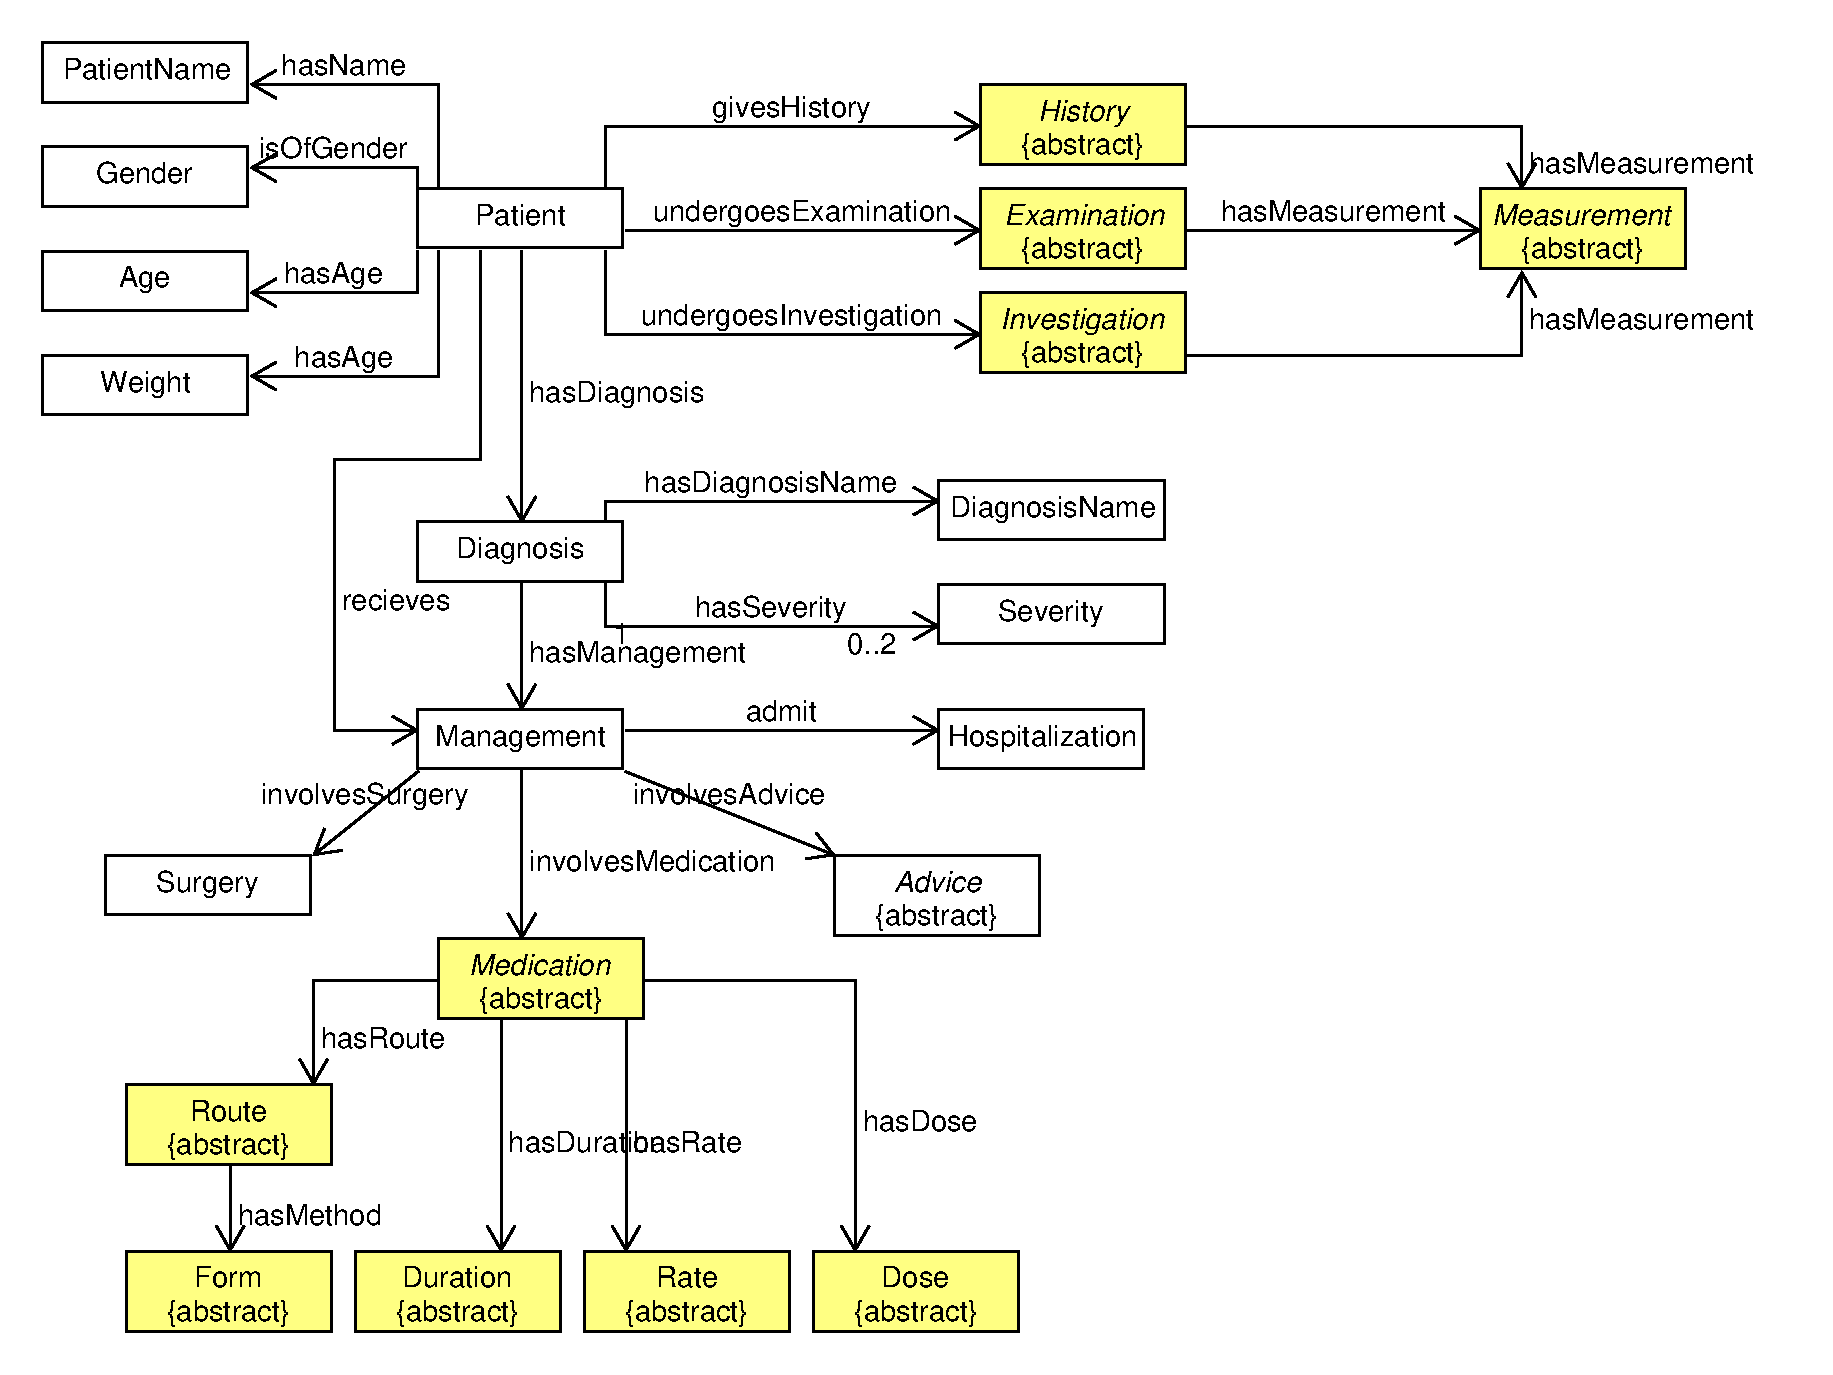
\includegraphics[scale=0.4]{GeneralEntityGraph}
	\caption {A generic entity graph contains abstractions. An entity graph for a specific guideline, contains specifications for those abstractions. Yellow boxes indicate specifications we have shown for paediatric guideline of possible asthma \parencite{RepublicofKeny2016}}
	\label{fig:GeneralEntityGraph}
\end{figure}

\section{Workflow model}
We model the dynamics of clinical encounters with a workflow model. The clinician starts with the assessment, where he examine the patient and listen to what the patient and the caregiver has to say about the the patient's condition. The clinician starts to get an idea of what condition the patient may suffer from. The clinician continues with the diagnostic part, where he asks more targeted questions to the patient and caregivers about the condition, do more of the examination and perhaps order lab tests as part of the investigation. This process can strengthen the clinician's assumptions about the condition, and he may be able to set a specific diagnosis.

The next step is the management and treatment. This can be changing the patient's status from outpatient to inpatient, do surgery, medication, physiotherapy, cognitive behavioural therapy or other forms of treatment. The treatment may be done in iterations or repeated.


The final step is to evaluate. The treatment may have to be adjusted to get the right effect. The diagnosis has changed. For example the severity of asthma may have changed from severe to mild or moderate after the treatment. Or we have initial set the wrong diagnosis, for example we have treated a patient for possible asthma, but in fact an object was stuck in the airways of the patient.


\begin{figure}[h!]
	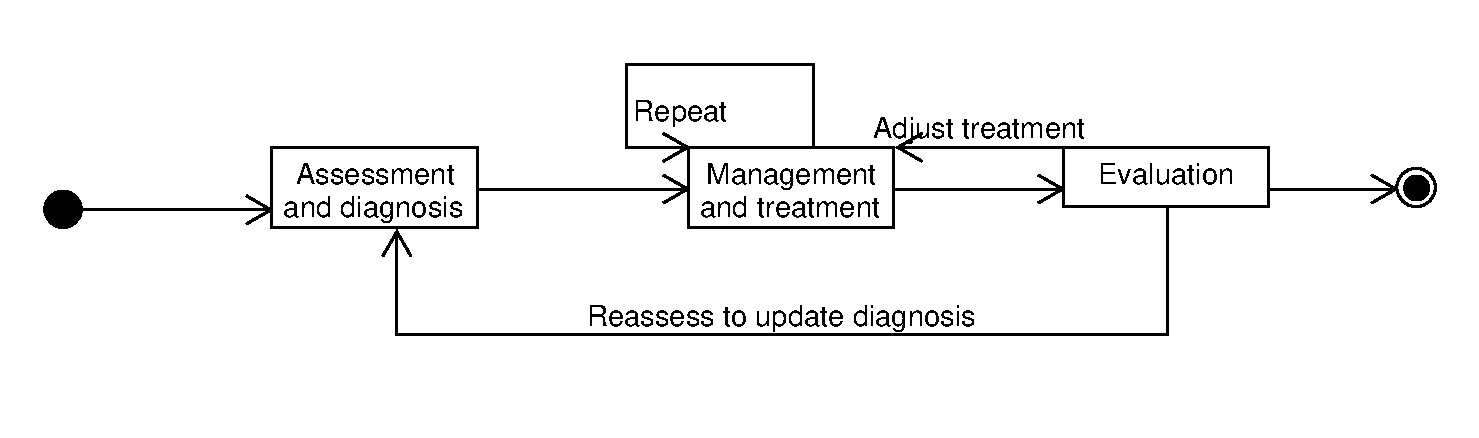
\includegraphics[scale=0.5]{WorkflowGraph}
	\caption {The workflow models is a model of the clinical encounter}
		\label{fig:WorkflowGraph}
\end{figure}

The idea of the workflow model is to describe the process of a clinical encounter. When making scenarios for the game, we know in which order the scenarios should come. The entity model is also connected to the workflow model. When doing a an assessment and diagnosis, you are looking at the examination, history and vertices of the entity model, where the diagnosis vertex answer to what the specific diagnosis is. For doing management and treatment, you look at the vertices under management in the entity model. An evaluation will be done by looking at the examination and investigation vertices to see if the patient has become better. The treatment needs to be adjusted accordingly to the evaluation. If the evaluation says we can't do more for the patient and there's no need for a follow-up, we exit the workflow model.

\textcolor{red}{Should perhaps reference to Rabbis articles here? 
	Coordination	of multiple metamodels, with application	to healthcare systems.
A flexible metamodelling approach for healthcare systems. }

\section{Metamodeling}

\textcolor{red}{I struggle when it comes to talking about MDE, DPF, metamodeling and model transformation, as I lack very basic knowledge about the subjects. Rutle, Rossini, Rabbi are all hard to read}

\textcolor{purple}{TODO: Yngve has a definition of metamodels which aren't so easy to read}

In figure \ref{fig:MetamodelEntityGraph}, we make an instance of the entity model. An instance of the entity model describes an actual patient at one point in the clinical encounter. 

For an instance to be valid, the vertices and edges have to correspond to a part of the model. We demonstrate this by adding dotted arrows in figure \ref{fig:MetamodelEntityGraph}. 

In figure \ref{fig:MetamodelEntityGraph} a patient tells the clinician that he struggles with a wheeze and a cough. Cough and Wheeze inherit from History in the model. Difficulty breathing is part of \ref{fig:EntityGraphHistory}, but is not represented here as the patient hasn't brought up this issue or been asked about it. We see how two inheritances og History translated in the instance from the model. The Measurement vertex holds the measurements of the History vertices. A patient with a wheeze and a cough is diagnosed with asthma, which is shown in the instance.

\begin{figure}[h!]
	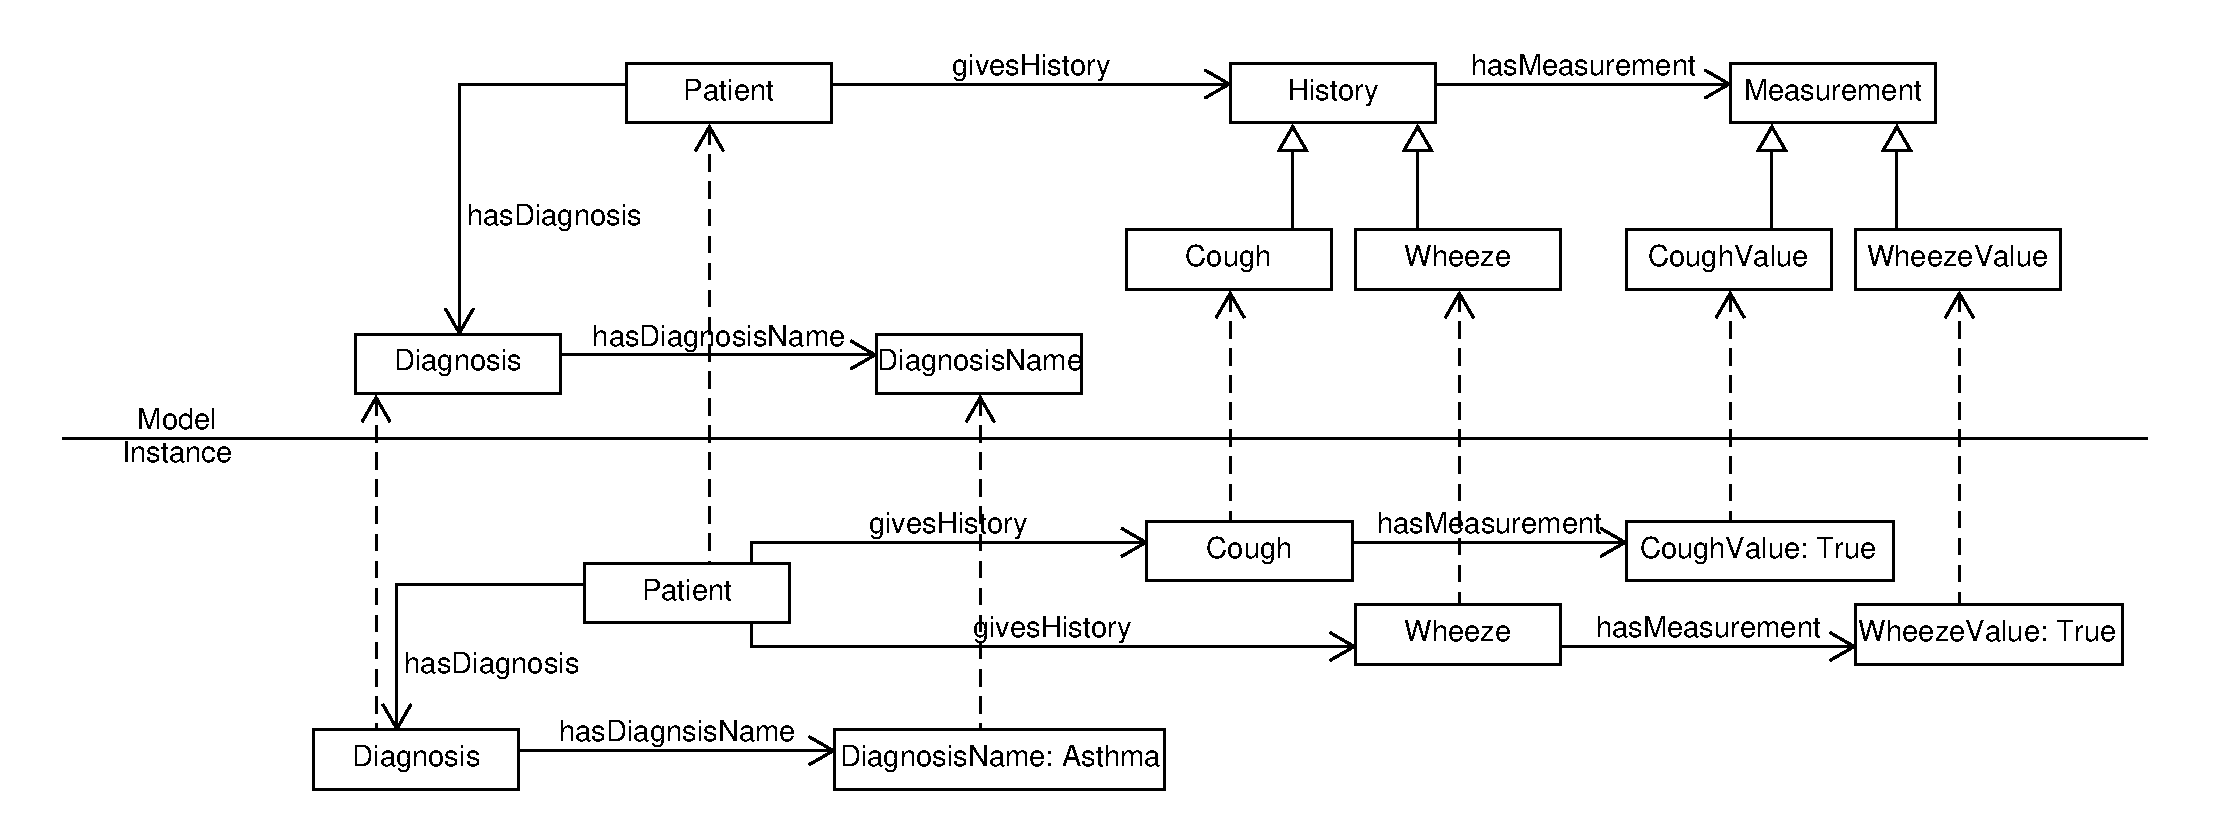
\includegraphics[scale=0.35]{MetamodelEntityGraph}
	\caption {A model and an instance of the entity model. For a valid instance, every vertex and edge in the instance has a corresponding vertex and edge in the model}
		\label{fig:MetamodelEntityGraph}
\end{figure}

\textcolor{purple}{TODO Yngve: shows where you are in guideline figure \ref{fig:MetamodelEntityGraph}}

In figure \ref{fig:IntegratedEntityWorkflowModels} we show a entity instance working together with the workflow model. For the assessment, we look at the History and Examination vertices. For Diagnosis, the DiagnosisName and Severity. Keep in mind that under Diagnosis, the clinician may do further examinations and questions to the patient to confirm his assumption, or which may cause him to think about other diagnosis. Management, the asthma is severe so we change the patient's status to inpatient by updating the Hospitalization vertex. We also look at the Medication vertex under Management. We only care about the medications for now in this example, and not how the medications should be administered. The Evaluation holds a reference to a new entity instance, which holds the updated information about the patient's symptoms. The clinician needs to act accordingly and adjust the treatment.

\begin{figure}[h!]
	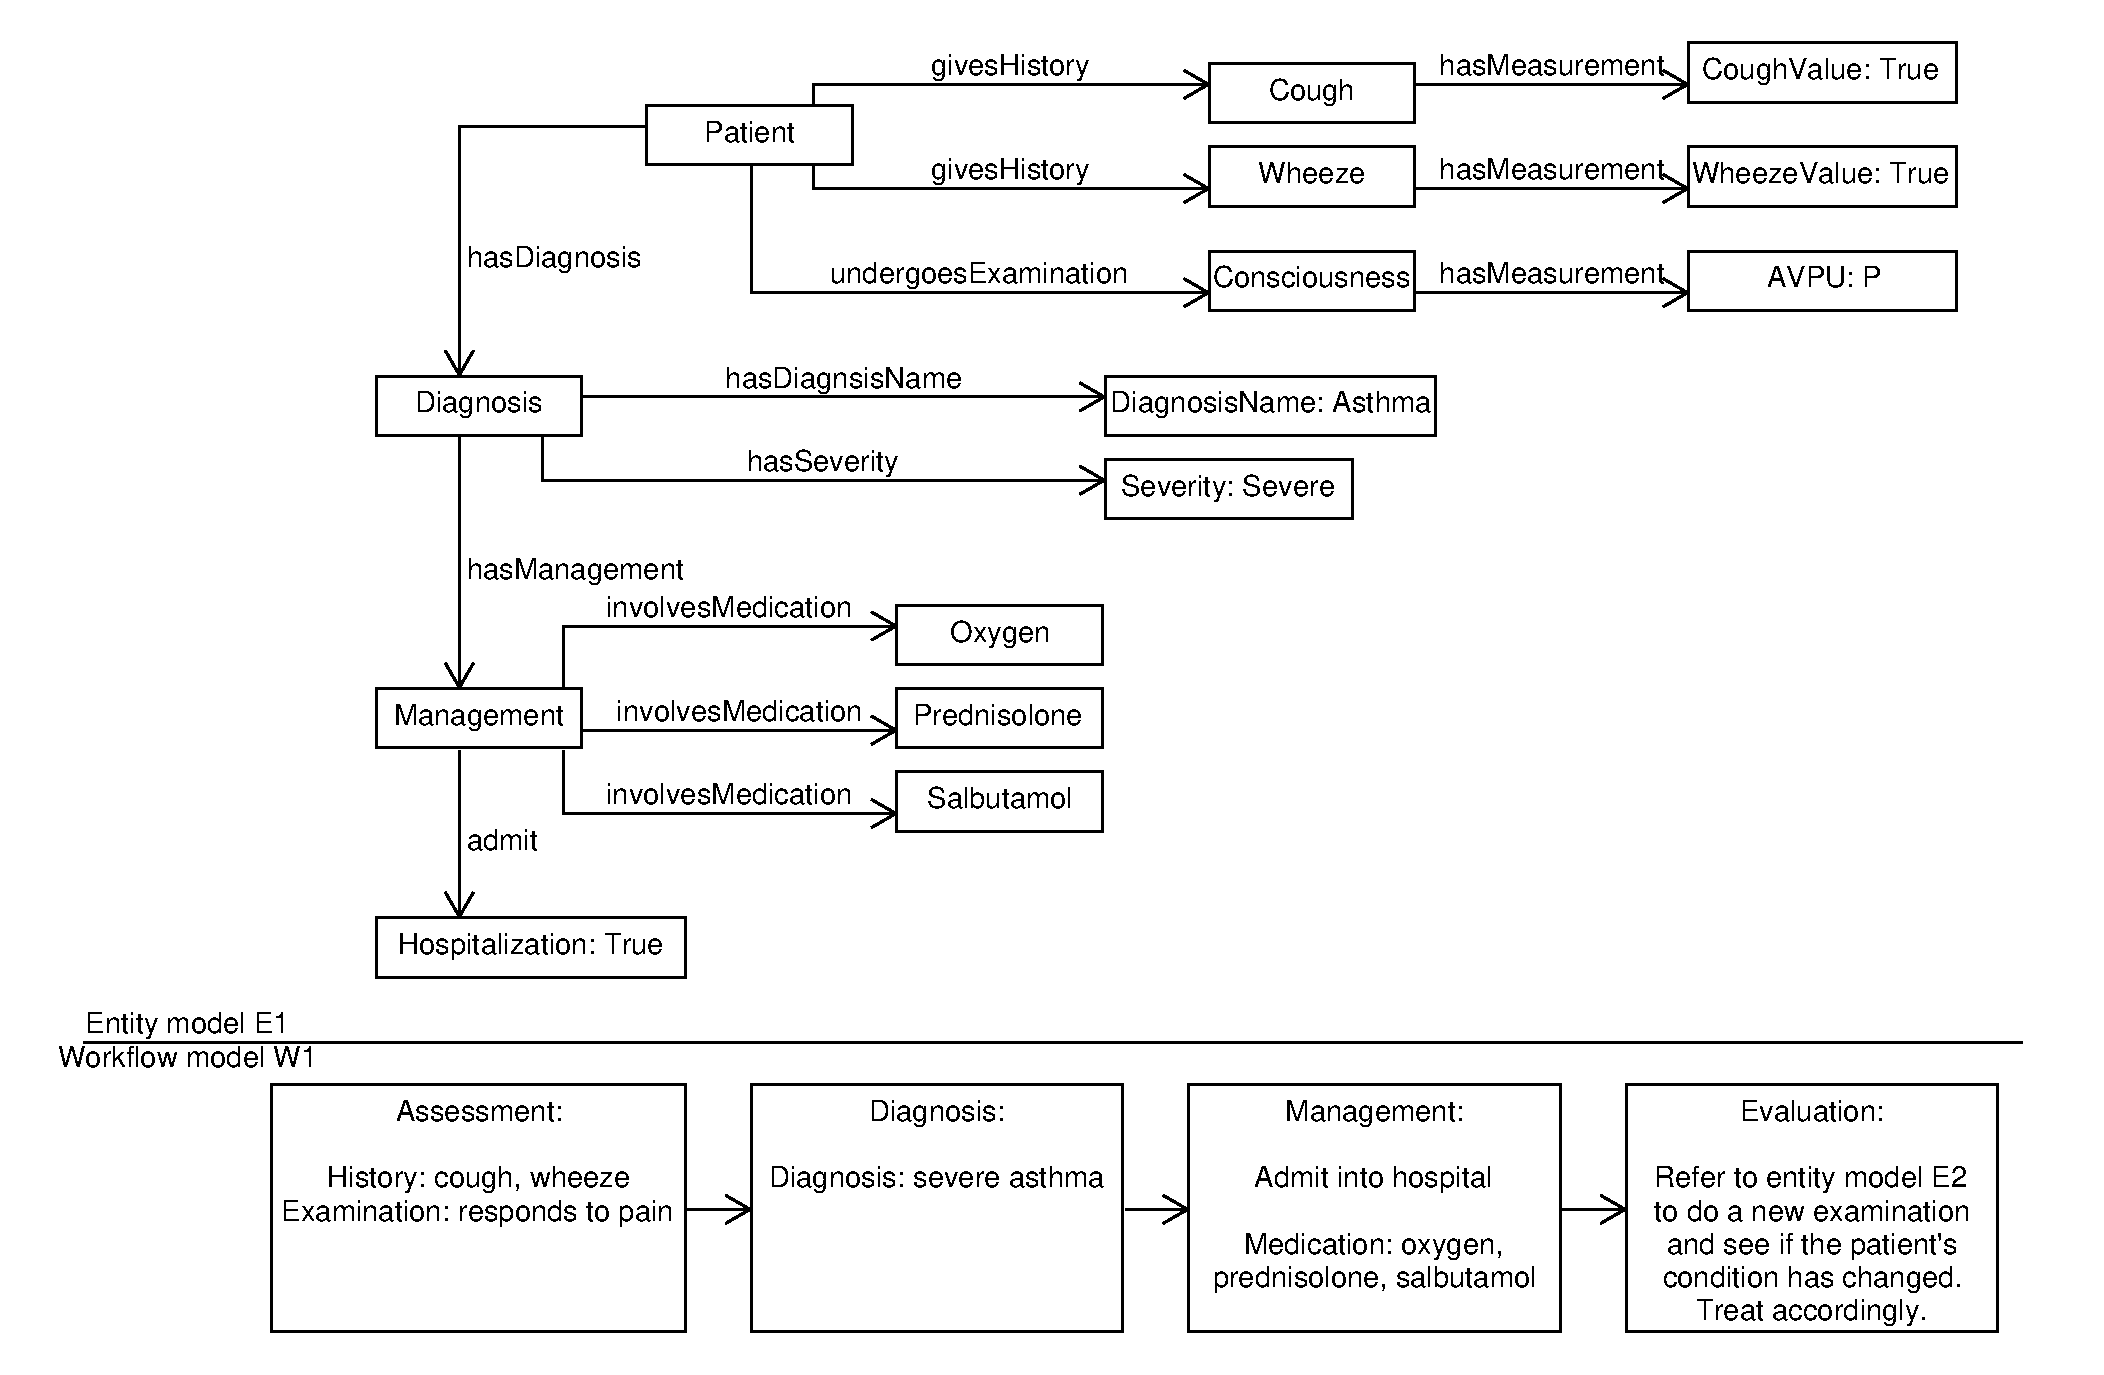
\includegraphics[scale=0.38]{IntegratedEntityWorkflowModels}
		\caption {An instance of the workflow model at the bottom, working together with an instance of the entity model at the top}
		\label{fig:IntegratedEntityWorkflowModels}
\end{figure}


\section{Game model}
The game model is not implemented using DPF and MDE like the entity model and workflow model. However, a MDE game model could be relevant in future work.

Here we will give a brief explanation of the content of the game model. It can work as a reference point for the next chapter, where we will discuss the game elements more thoroughly.
\begin{itemize}
	\item \textbf{Category:} a CPG is written for a specific medical condition. The quiz category will be the medical condition, or the name of the CPG the quiz is written for.
	\item \textbf{Discipline:} a question is written for a specific step in the clinical encounter, which the workflow model is an abstraction of. Discipline is a step in the clinical encounter.
	\item \textbf{Level}: Is the difficulty level of the question.
	\item \textbf{Passing condition:} a condition the student has to fulfil to pass a specific  difficulty level.
	\item \textbf{Required Minimum Skill:} a condition the student has to fulfil to be able to play questions at a specific difficulty level.
	\item\textbf{Entity Instance}: a pointer to an instance of an entity graph. It is used together with a template to generate text.
	\item \textbf{Question:} a pointer to a template model. By using a template model, we can reuse templates on many entity instances.
	\item \textbf{Alternative:} or distraction. It is one of the answer alternatives for a question. 
	\item \textbf{Reward:} a reward or penalty is given based on the correctness of the distraction. A distraction can be degrees of right or wrong, which is reflected by the reward.	
\end{itemize} 

The game model is paired with a template model. By separating the template into its own model, we can reuse the same template for many questions.
\begin{itemize}
	\item \textbf{Narrative:} template which represents a question. The template contains tags which points to vertices in an entity graph. When the template is paired with an instance of such a graph, it will produce a textual presentation of a question. The same template can be used with different instances of entity graphs to make many different questions.
	\item \textbf{Answer key:} is a tag which points to a vertex in the entity graph. When paired with an instance of the entity graph, it will produce a textual presentation of the answer key. The answer key can be used with many different entity graph instances.
	\item \textbf{Explanation:} this is the answer key explanation to a narrative/question. It gives an description of how to solve the problem and what is the correct answer.
	\item \textbf{Evidence and Guideline:} these are not implemented yet, but are place-holders for future functionality. The evidence is the strength of the evidence the recommendations in the guideline. The guideline is a pointer to the guideline itself. Such that that the student can read the guideline itself when he is stuck on a question or need further explanation. This will hopefully enforce learning.
\end{itemize}

\section{Student learning model}
The student learning model keeps track of the student's scores at different quizzes. It is based on the principles of learning map and student map, which can be read about in the next chapter about game elements. By using such a model, we can adapt the questions to the right difficulty level for the student. We can also keep track of his progression

\section{Summary}
In this chapter we have discussed the entity-, workflow-, game- and student learning models. We have been especially thorough with the two first models, which are developed using MDE and DPF. In MDE it is the models which drives the development process, and DPF is an approach to MDE where the models are represented as a graph with a set of constraints.

In the entity model, we modelled the patient, the symptoms the clinician might find under examination and by the history the patient or parents give. We modelled the diagnosis, and how the clinicians manage thee medical condition of the patient. The clinician may admit the patient into the hospital, treat with medications and give some advise on how the patient or parents should manage the medical condition of the patient.

A workflow model which is the workflow of the clinical encounter.

We do an example where we make instances of the entity model my metamodelling. Then we instantiates the entity model together with the workflow model, to see how they work together. Describing the patient, the condition, symptoms and the management through the whole clinical encounter. Through assessment and diagnosis to management and treatment to evaluation.

We gave a brief explanation of the elements in the game model, and the concept of the student learning model. 


\chapter{Game Elements}

In this chapter we will try to relate the sections to the conceptual managers in the game engine. The reason for doing this is to easier identify and describe the different responsibilites the game engine has:
\begin{itemize}
	\item \textbf{Question flow manager}: adapts the questions to the knowledge level of the student, and is flexible such that the student can choose his own path through the completion of each difficulty level. 
	\item \textbf{Conversation manager:} puts the questions with belonging answer elements in a sequence such that they fit to a scenario, using the workflow model. The conversation manager produces questions and answer keys from a template, in which the entity model is used to fill in data for the place holders in the template.
	\item \textbf{User manager:} keeps track of the user's skill, based on the performance on previous quizzes. It holds track of the scores on the current quiz, and it measures the user's progression.
\end{itemize}


\section{Question Flow Manager}

% -----------------------------------------------------------------------------------------------


As each question in a quiz are related to a certain component in the treatment plan or theme in the learning map, the student will be measured how well he performs on each of these themes. For the asthma guideline \parencite{RepublicofKeny2016}, we have identified four themes. Assessment where the student will be tested in the initial examination. Diagnosis, where the student will determine a diagnosis as well as the severity. Management, where the student will determine which actions should be done to treat and best give the best care to the patient. The last discipline is the follow-up, where the student will be tested in evaluating the treatment, give advise to and educate patient and caregivers, provide the right medication and regular follow-up.

By splitting up the score in themes, the student can easily see which areas he is strong and where he needs more training. 



We can also adapt the questions in each discipline to the student's level. If the student has proven to be very good in providing the right amount of medicine to asthma patient, we can provide more difficult questions to challenge the student some more. If he struggles at setting the right diagnose, we can provide more basic questions to strengthen the students basic knowledge. 




The student will also be provided with a total score, which will be the aggregated score of each of the disciplines. The student can compare the total score of e.g. the asthma quiz and the jaundice quiz, and see which medical condition he needs to train more on.



\subsection{Dynamic Content Management}
The game engine is based on some of the concepts presented in the articles of \textcite{Eide2008}, \textcite{Kristensen2011} and \textcite{Kristensen2013}. The motivation for using DCM, is to support the principles of adaptive learning as well as flexibility in the learning process. Adaptive learning means that the student can solve problems which are suited to his knowledge level. Flexibility in the sense that the student can go through the learning content in many different ways.

\textcite{Eide2008} presents a dynamic content management system (DCM) made for e-learning. In DCM the focus is on removing the tight coupling between the learning material and the teaching course. By analysing the learning material and course, they can define conceptual atomic units of knowledge which they put into a knowledge repository. From this repository they may draw knowledge elements and organize into the hierarchy of a course. To model a course they use concept maps, which are directed graphs, where the vertices are concept labels and edges indicates the relationships between vertices. DCM operates with three concept maps: knowledge map, learning map and student map. The knowledge map is used to model the entire content of the knowledge repository and the hierarchy structure of a course. A learning map is used to model a specific course and is a representation of the learning process. The content units (vertices) in the knowledge map gets expanded, and becomes evaluation and resource vertices in the learning map. Content units from the knowledge map can be omitted if they are not needed in the specific course. Detailed prerequisites can be specified for the content units. The student map represents the progress of a specific student taking a specific course. The edges shows which resources he has used, the evaluations of the student and in which order. 


When we apply this to our project, we will first decouple the content from the flow-chart of the paediatric possible asthma guideline \parencite{RepublicofKeny2016}. To decouple the flow-chart, we use the workflow model as a helping tool, ordering on how they should learn the clinical guideline. In figure \ref{fig:KnowledgeMap} we have identified knowledge elements and hierarchically structured the knowledge repository into a knowledge map. The edges shows the dependencies in the learning process. To learn how to evaluate a treatment and act accordingly to the evaluation, the student needs to know something about how to set a diagnosis and how to initially treat it. Hence there is an edge between follow-up and the other knowledge units.

\begin{figure}[h!]
	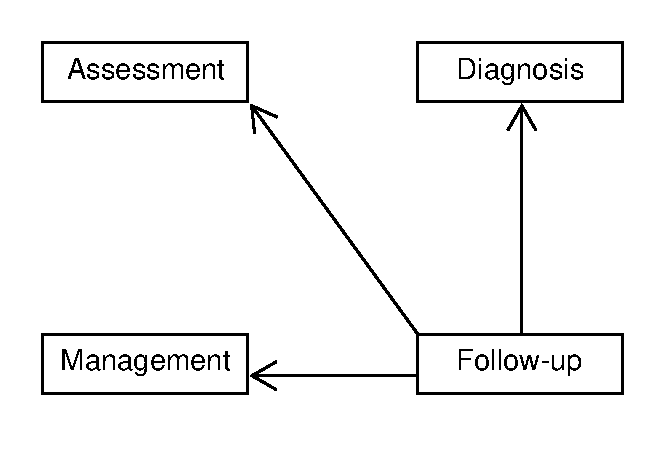
\includegraphics[scale=0.6]{KnowledgeMap3}
	\caption {Knowledge map}
	\label{fig:KnowledgeMap}
\end{figure}

In table \ref{table:ContentUnit} we have chosen a knowledge element from the knowledge map, and defined a content unit. The content unit contains a theme "Assessment". Resources is the learning material, which are relevant sections of the guideline. Evaluations are the tests to see if the student has reached the learning goals. At level 1 we try to learn facts about the guideline. In level 2 and 3 we give the student scenarios to work with.

\begin{table}[h!]
	\begin{tabular}{ | m{14em} | m{9em}| m{5em} | } 
		\hline
		\multicolumn{3}{c}{\bfseries T1: Assessment} \\
		\hline
		Resources & Evaluations & Aspects \\
		\hline
		R1: History and examination sections in the possible asthma guideline \parencite{RepublicofKeny2016} & E1: Quiz Level 1 & Facts \\
		& E2: Quiz Level 2 & Scenario \\
		& E3: Quiz Level 3 & Scenario \\
		\hline
	\end{tabular}
	\caption{The content unit Assessment}
	\label{table:ContentUnit}
\end{table}

In figure \ref{fig:LearningMap} we have identified four content units T1: Assessment, T2: Diagnosis, T3: Management and T4: Follow-up from the knowledge map. The importance of these content units in the asthma guideline \parencite{RepublicofKeny2016} was the reason these four got selected. The hierarchically structure of the knowledge map, makes the child nodes of the content units become learning material for their parent nodes.

Inside the content units in the learning map, we see the relationships between resources and evaluation. There is also dependencies between the content units. To be able to do a follow-up, a student needs to learn the assessment, diagnosis and management first, because follow-up is an evaluation and reaction to how the patient responded to the previous steps.  We have also specified the prerequisites for each evaluation. The prerequisites are written as logical expressions, as seven edges and operators per content unit would be confusing to read. What the prerequisites says is that all level 1 evaluations need to be completed before any level 2 evaluation can be taken. All level 2 evaluations need to be completed before any level 3 evaluation can be taken.

\begin{figure}[h!]
	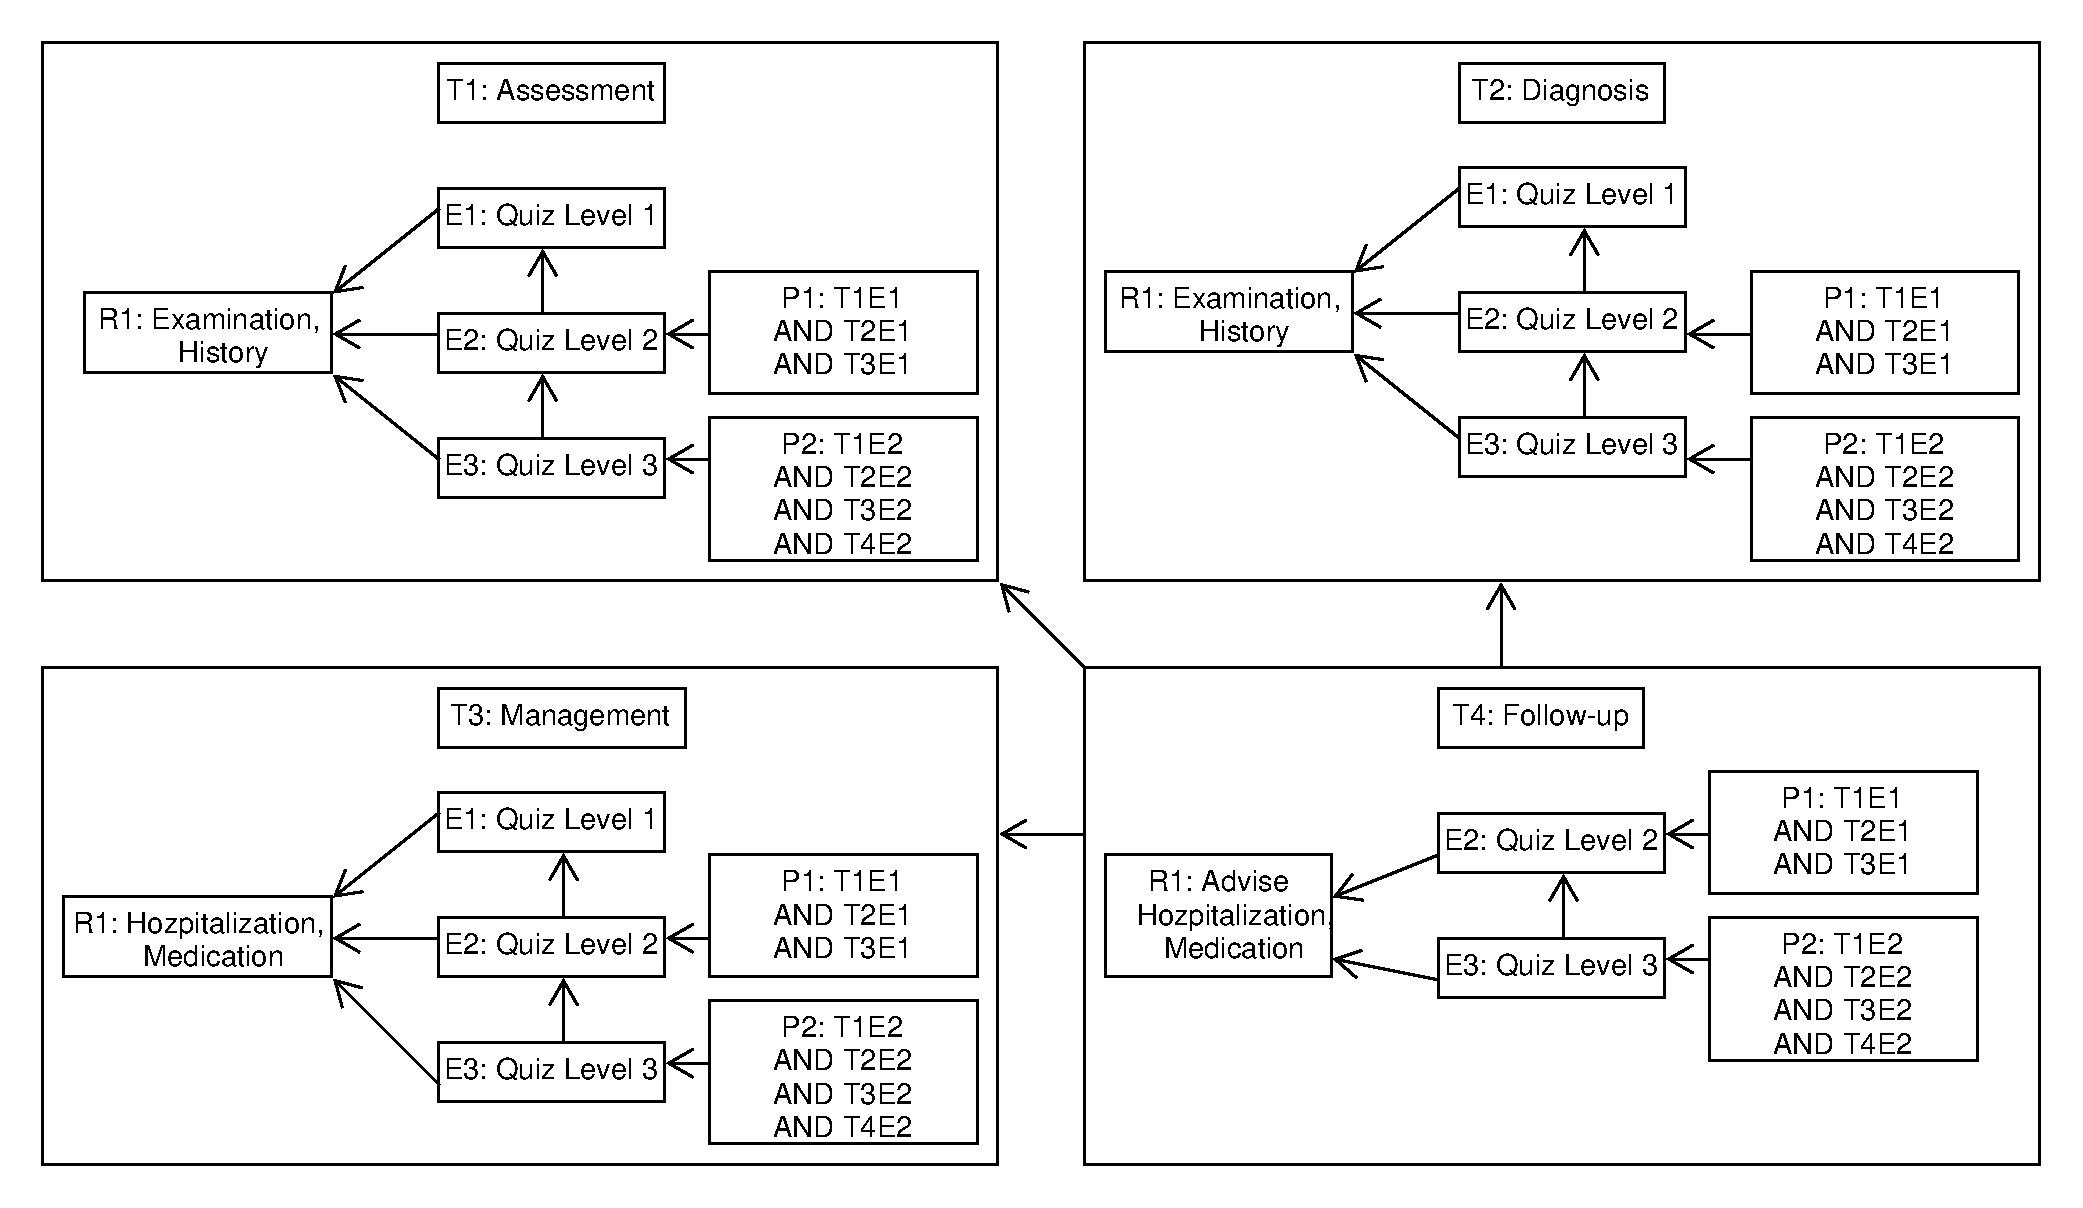
\includegraphics[scale=0.38]{LearningMap}
	\caption {Learning map}
	\label{fig:LearningMap}
\end{figure}

A student map would show the progressions for one specific student, and the path he has taken and the scores for each evaluation. Table \ref{table:StudentMap} shows a student's student map for the Assessment part of the course. He got the score 34 on the first evaluation. 34 matches the passing condition for assessment level 1, so he got a passing grade for that test. However, he scored 43 points on evaluation 2 and didn't meet the passing condition for that test. He has no attempts for evaluation 3, as he doesn't meet the prerequisites for that test.  The tests which have been completed are stored in the database on the students phone. In that sense, the database shows the student's current position in the learning map.

\begin{table}[h!]
	\begin{tabular}{ | m{12em} | m{8em}| m{5em} | } 
		\hline
		\multicolumn{3}{c}{\bfseries T1: Assessment} \\
		\hline
		Resources & Evaluations & Passed \\
		\hline
		R1: History and examination guideline & E1: 35 & True \\
		& E2: 43 & False \\
		& E3: &  \\
		\hline
	\end{tabular}
	\caption{Student Map T1:Assessment}
	\label{table:StudentMap}
\end{table}

\subsection{Types of questions}
We can further identify which kind of questions we are going to ask, by further examining the entity model and the workflow model combined. When we are doing an assessment in the workflow model, we are looking at the examination and history vertices of the entity graph. History is what the patient or the patient's dependent can tell around the patient's condition. Such that he has been coughing a lot the last days. Examination and history will provide the clinician with an idea of a diagnosis.

Diagnosis in the workflow model is connected to the history, examination and investigation. The clinician will continue asking questions, do examinations and probably order some tests to strengthen his assumption of the diagnosis. The clinician can also set a more specific diagnosis, such as in the asthma guideline \parencite{RepublicofKeny2016}, where we categorize in severe, mild and moderate asthma.

Management is how we manage the patient with the given diagnosis. Hospitalization is if we are going to set patient status to inpatient or outpatient. Medication is given to treat the patient or relieve the symptoms. Surgery is not part of the asthma guideline \parencite{RepublicofKeny2016}, but it is important to be aware that management procedures needs to be added when making quizzes for other conditions than asthma.

Follow-up will contain questions related how to evaluate the treatment and how to act upon the evaluation. The symptoms of the patient may have worsen, getting better or are unchanged after the treatment, and the clinician needs to act accordingly. The treatment may have been given at the hospital or it may have been something the patient have had to do at home. The patient may also get some instructions from the clinician when there is something he should do on his own.

\begin{figure}[h!]
	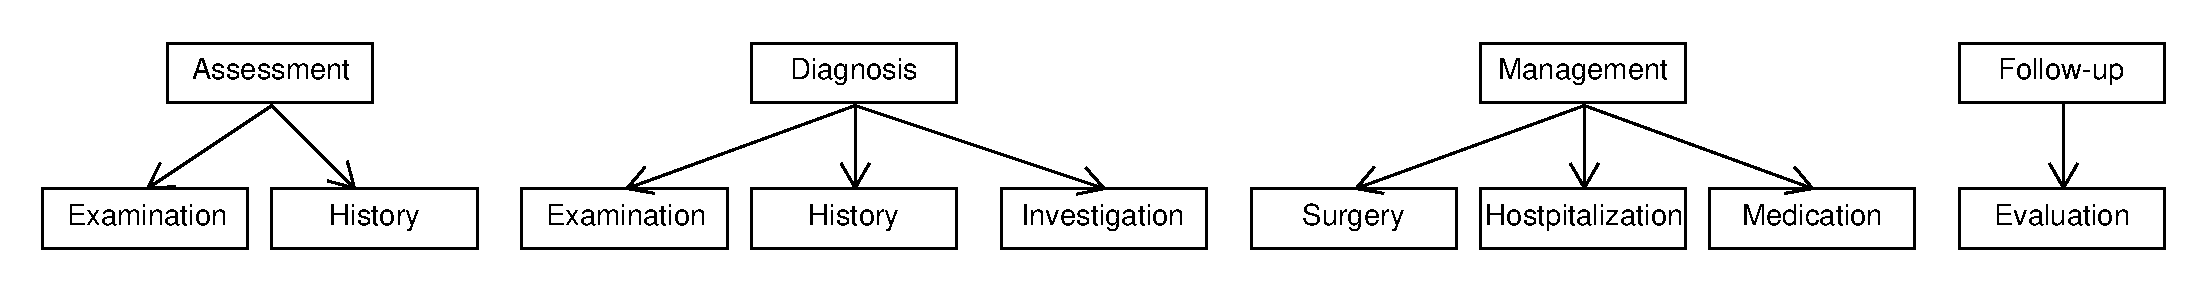
\includegraphics[scale=0.36]{KnowledgeMap2}
	\caption {By looking at the workflow- and entity models we can identify the type of questions for each content unit in the knowledge map. The content units are the parent nodes, while the leaves are the type of questions}
	\label{fig:ExpandedKnowledgeMap}
\end{figure}

As the student learns, the questions need to adapt to the student's new level of knowledge. How we do this is by defining levels, where the questions becomes more detailed at higher levels. At level 1 the questions are all about stating facts. In level 2, we create scenarios such that we follow one patient through all of the steps assessment, diagnosis, management and follow-up. The same for level 3, but the detail level will be higher. Typically the student will only be asked for categories of medication in level 2, but in level 3 the students needs to be specific about the names of the medication as well as measurements for both dosages and symptoms. See table \ref{table:ProgressionGranularity}.

\begin{table}[h!]	
	\begin{tabular}{|m{2em}|m{6em}|m{6em}|m{6em}|m{6em}|}
		\hline
		Level & Assessment & Diagnosis & Management & Follow-up \\
		\hline
		1  & Factual & Factual & Factual & - \\
		2 & Scenario & Scenario & Scenario & Scenario \\
		3 & Detailed scenario  & Detailed scenario & Detailed scenario & Detailed scenario \\
		\hline
	\end{tabular}
	\caption{The type of questions at each difficulty level}
	\label{table:ProgressionGranularity}
\end{table}




\subsection{Unlocking harder levels at a certain category}
One of the strengths with Dynamic Content Management is the focus on adaptive learning and flexible learning \parencite{Eide2008}. By adaptive learning, we mean that the student can solve problems which are suited for his knowledge level. While flexible learning means that the student can go through the learning material in the way he prefers, as long as the knowledge dependencies are met.

For the adaptability we have already covered how we progress from factual statements to scenarios and the scenarios with a higher ability to make the questions more difficult. For the flexibility we have divided the content into knowledge units: assessment, diagnosis, management and follow-up. It doesn't matter which of assessment, diagnosis and management the student finishes first.

The evaluations in each content unit has passing conditions. As an example; to complete assessment level 1, you need a score of 30 in assessment. These passing conditions are provided by the quiz author. We also recall that to unlock questions, such as management level 2, there are certain prerequisites that need to be fulfilled. In this example, all evaluations in level 1 need to be completed to unlock any level 2 questions. The flexibility is that it doesn't matter the order of level 1 evaluations the student finishes first, as long as all of them are finished.

To avoid that the student gets bored, he will not have to redo an evaluation once the passing condition is met. That means that if the student meets the passing condition of level 1 assessment and diagnosis, but not management, the student will only get questions from management level 1 the next time he takes the quiz. This makes a challenge for the scenarios. All scenario questions must be formed in a way, such that the student doesn't have to remember information from one question to another. All the necessary information should be listed in every scenario question. In that way the student won't miss important information if he completes diagnosis in a run before management and follow-up. 

Each evaluation also has a minimum required skill value. If the student gets a lower score than the required minimum skill, the evaluation gets locked and the student needs to complete the evaluation at lower level. An example is that the student plays management level 2. He completes the evaluation with a lower score than the required minimum skill. The student will have to redo management level 1 evaluation to learn the basic skills necessary to play level 2. When this situation happens, the student no longer meets the prerequisite for the other level 2 evaluations. Level 1 management needs to be completed before any level 2 evaluations can be taken. 





\section{Conversation Manager}
\subsection{Constructing scenarios and answer keys}
A quiz consists of several questions, where each question has answer keys and distractions. At level 1 these questions will be factual, and in level 2 and 3 we will work with scenarios. We write the questions in the format of a template, where we use tags to refer to variables in the entity model. The tag is a path in the entity graph. The game engine will traverse through the graph and return the value of the vertex specified by the path. The entity graph represents a patient at a certain point in the assessment or treatment. By replacing the entity graph, we can reuse the same template with different patients, generating many different questions with the same template. 

The same goes for the answer key. The answer key can be a text, one or several tags referring to variables in the entity model, or a combination of both. The application always uses the same entity graph for the scenario and the answer key. When the application traverses entity graph, the answer key and the question given always matches as they are the same patient at the same given time.

One of the problems we encountered with this method, was how to present the variables returned by the graph in a text. As an example, we can look at some of the symptoms of asthma and their type.
\begin{itemize}
	\item Wheeze is a whistling sound when you breath. In the model it is represented as a boolean. True or false. Either you have it or you don't.
	\item Age is relevant several places in the guideline. In the model it is stored as an integer.
	\item AVPU is a scale system, which clinician use to measure a patient's level of conciousness. A is alert. V, the patient is verbal which means he can somehow respond to questions. P, the patient responds to pain. The patient will react if you pinch him. U is unresponsive or unconscious. He doesn't respond to either voice or pain. The AVPU is represented in the model as an enumerate.
	\item Severity classifies the asthma severity to be either severe, model or mild. The severity is represented as a string in the model.
\end{itemize}

\begin{figure}[h!]
	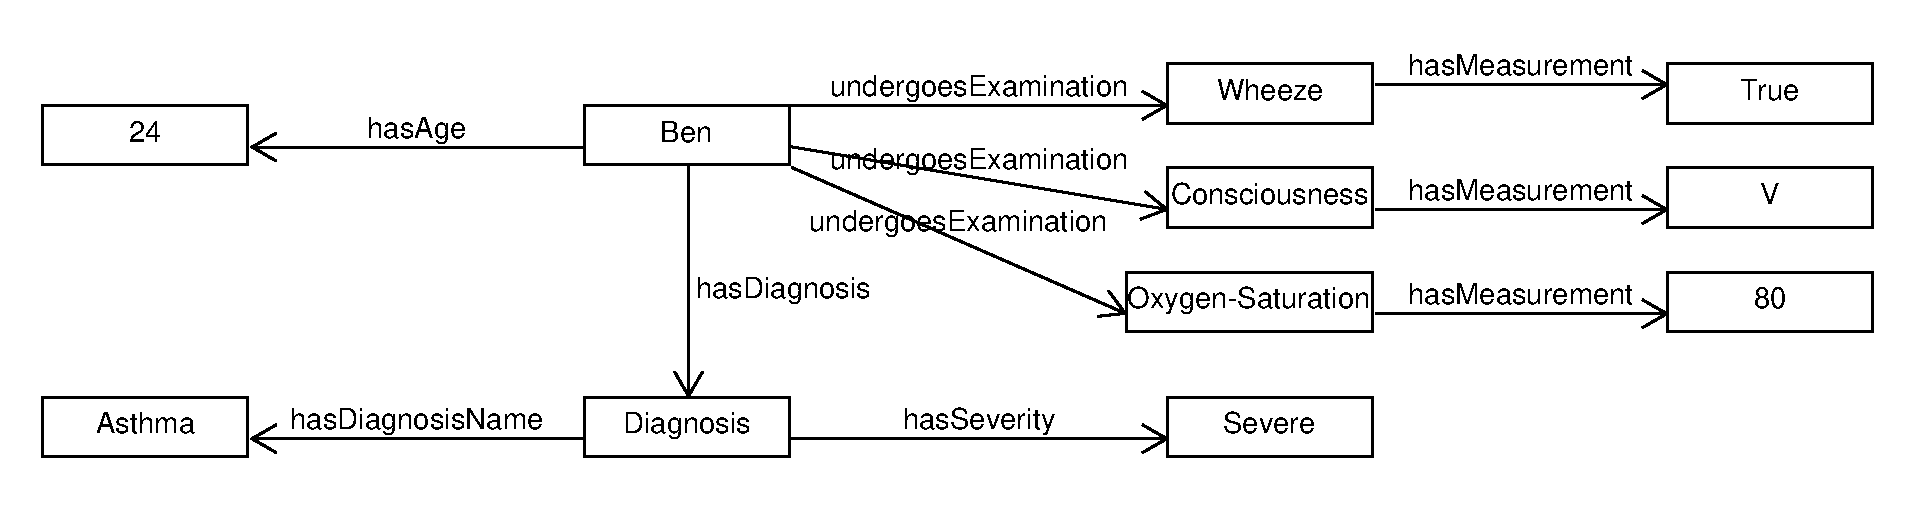
\includegraphics[scale=0.4]{EntityInstanceGraph}
	\caption {The patient object used with the template}
	\label{fig:EntityInstanceGraph}
\end{figure}

%\begin{lstlisting}[caption={My Caption},captionpos=b]
\begin{lstlisting}[caption={Question template}, frame=single, captionpos=b] 
Question:
A <%Patient.hasAge.Age%> months old patient arrives at 
the  emergency department. 
The patient has a 
<%Patient.underGoesExamination.Wheeze%>,
has conciousness level 
<%Patient.undergoesExamination.Consciousness%> 
and has an oxygen saturation of 
<%Patient.undergoesExamination.Oxygen-Saturation%>%. 
What is the asthma severity? 
\end{lstlisting}

\begin{lstlisting}[caption={Answer key template}, frame=single, captionpos=b] 
Answer key:
<%Patient.hasDiagnosis.Diagnosis.hasSeverity.Severity%>
\end{lstlisting}

This translates to 
\begin{lstlisting}[caption={Question instantiation}, frame=single, captionpos=b] 
Question:
A 24 months old patient arrives at the emergency 
department. 
The patient has a true,
has conciousness level V 
and has an oxygen saturation of 80%. 
What is the asthma severity? 
\end{lstlisting}

\begin{lstlisting}[caption={Answer key template}, frame=single, captionpos=b] 
Answer key:
Severe
\end{lstlisting}

We see that the template author needs to be aware of how the variables will be printed. Here he knows that the model will just return an integer for the oxygen saturation. He writes a descriptive text of the value first, and then adds a percentage after the variable. The severity gets nicely printed as answer key.

The problem is the boolean for wheeze, which prints a "true". It really should have printed "wheeze". We solved the presentation of consciousness in the same way as we did with oxygen saturation. However, it could be nicer to write "responds to pain", rather than just "V". When the child 12 months or older, it is often easier to read if we can present the age in years.

Another problem arrives when we replace the entity graph with another, where some of the examinations haven't been done. In traditional model driven engineering, we use something called the closed world assumption \parencite{Sadowska2019}. If a node doesn't exist, we say the value is false. But how can we say that patient doesn't have wheeze when we haven't examined? In open world assumption a none-existing vertex is "unknown" \parencite{Patel-Schneider2006} \parencite{Bergman2018}, and this strategy seems more correct for our scenario. If the vertex doesn't exist, we simply return an empty string. This further motivates us to remove the variable specific text from the template, as we don't want text representation for a variable we don't present. Example when consciousness and oxygen saturation haven't been examined:

\begin{lstlisting}[caption={Question instantiation}, frame=single, captionpos=b] 
Question:
A 24 months old patient arrives at the emergency 
department. 
The patient has a true, has conciousness level 
and has an oxygen saturation of %. 
What is the asthma severity? 
\end{lstlisting}

How we solved the problem was to add a textual presentation vertex to each of the vertices in the graph referred to by the template. If there exist a presentation for the vertex, return the presentation. If there doesn't exist a presentation, simply return the variable.

\begin{figure}[h!]
	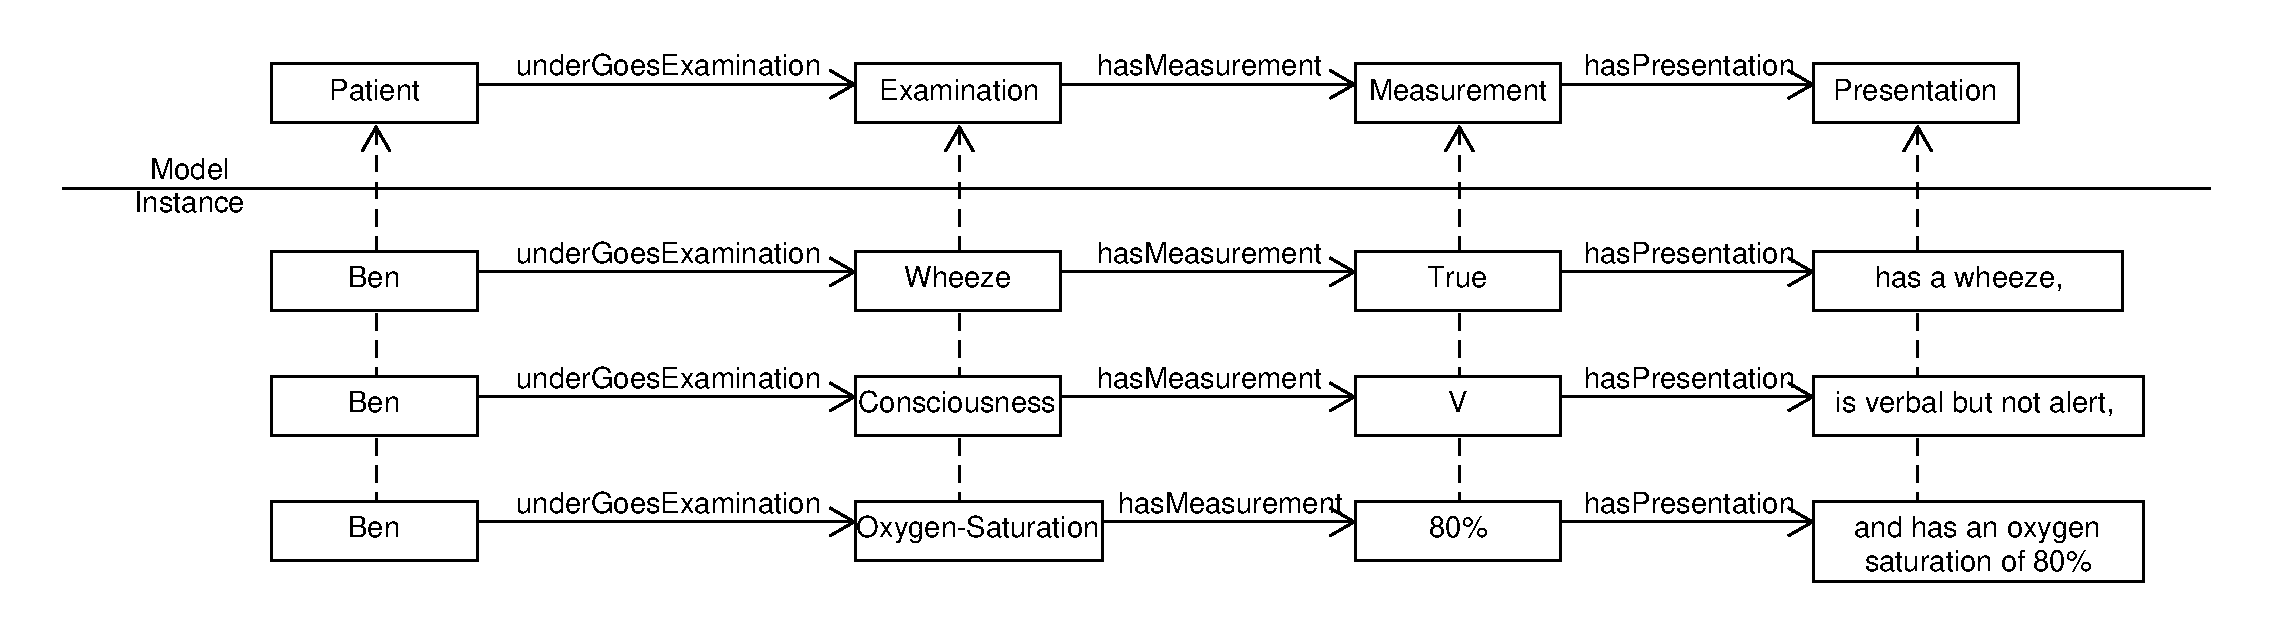
\includegraphics[scale=0.35]{GeneratingScenarios1}
	\caption {Making graph variables fit a story format}
	\label{fig:GeneratingScenarios1}
\end{figure}

\begin{figure}[h!]
	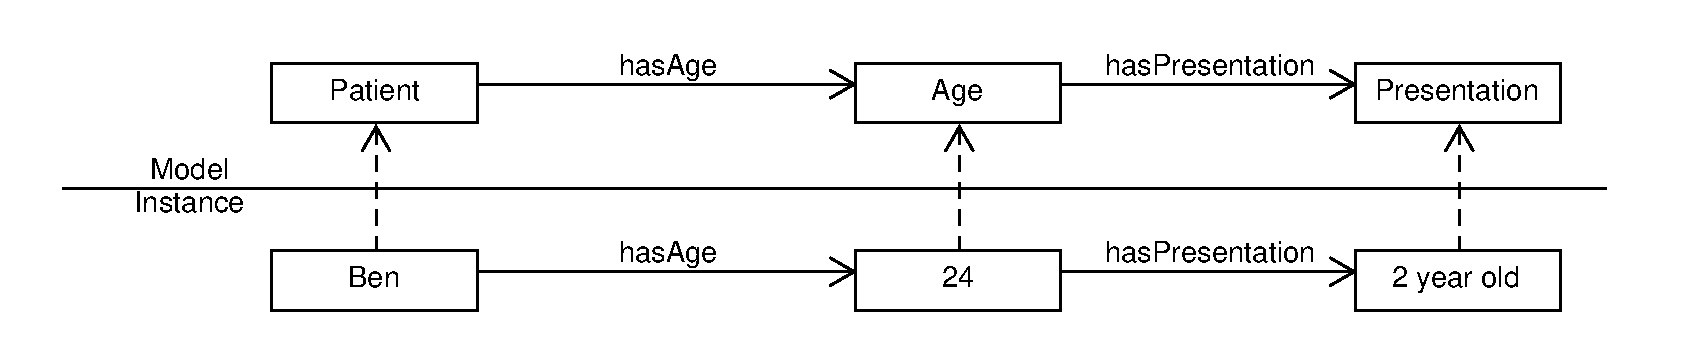
\includegraphics[scale=0.4]{GeneratingScenarios2}
	\caption {Making graph variables fit a story format}
	\label{fig:GeneratingScenarios2}
\end{figure}

\begin{lstlisting}[caption={Question template}, frame=single, captionpos=b] 
A <%Patient.hasAge.Age%> old patient arrives at 
the emergency department. 
The patient <%Patient.underGoesExamination.Wheeze%> 
<%Patient.undergoesExamination.Consciousness%> 
<%Patient.undergoesExamination.Oxygen-Saturation%>. 
What is the asthma severity? 
\end{lstlisting}

Which translates to 
\begin{lstlisting}[caption={Question instantiation}, frame=single, captionpos=b] 
A 2 year old patient arrives at the 
emergency department. 
The patient has a wheeze, is verbal but not alert 
and has an oxygen saturation of 80%. 
What is the asthma severity? 
\end{lstlisting}

This also works with the open world assumption, as a patient which haven't undergone consciousness and oxygen saturation examinations, would result in the following text:

\begin{lstlisting}[caption={Question instantiation}, frame=single, captionpos=b] 
A 2 year old patient arrives at the emergency 
department. 
The patient has a wheeze. 
What is the asthma severity? 
\end{lstlisting}

For future work, the commas and "and" should not be in the presentation vertex. This becomes a limitation where the variable can only be used in a list and has to be in a specific place in the list. The solution would be to have a list tag in the template, and have all the paths inside that tag. Then the game engine can see how many of the list items are in the graph, and can set the commas and "and" at the appropriate places.

In figure \ref{fig:IntegratedEntityGamelModels} we show how the entity-, workflow and game models work together to make a scenario. Because of limited space, we don't show the presentation vertices in the entity graph. We also combined entity graph E1 and E2 in the presentation, where E2 gets and additional medication vertex marked with red. 

\begin{figure}[h!]
	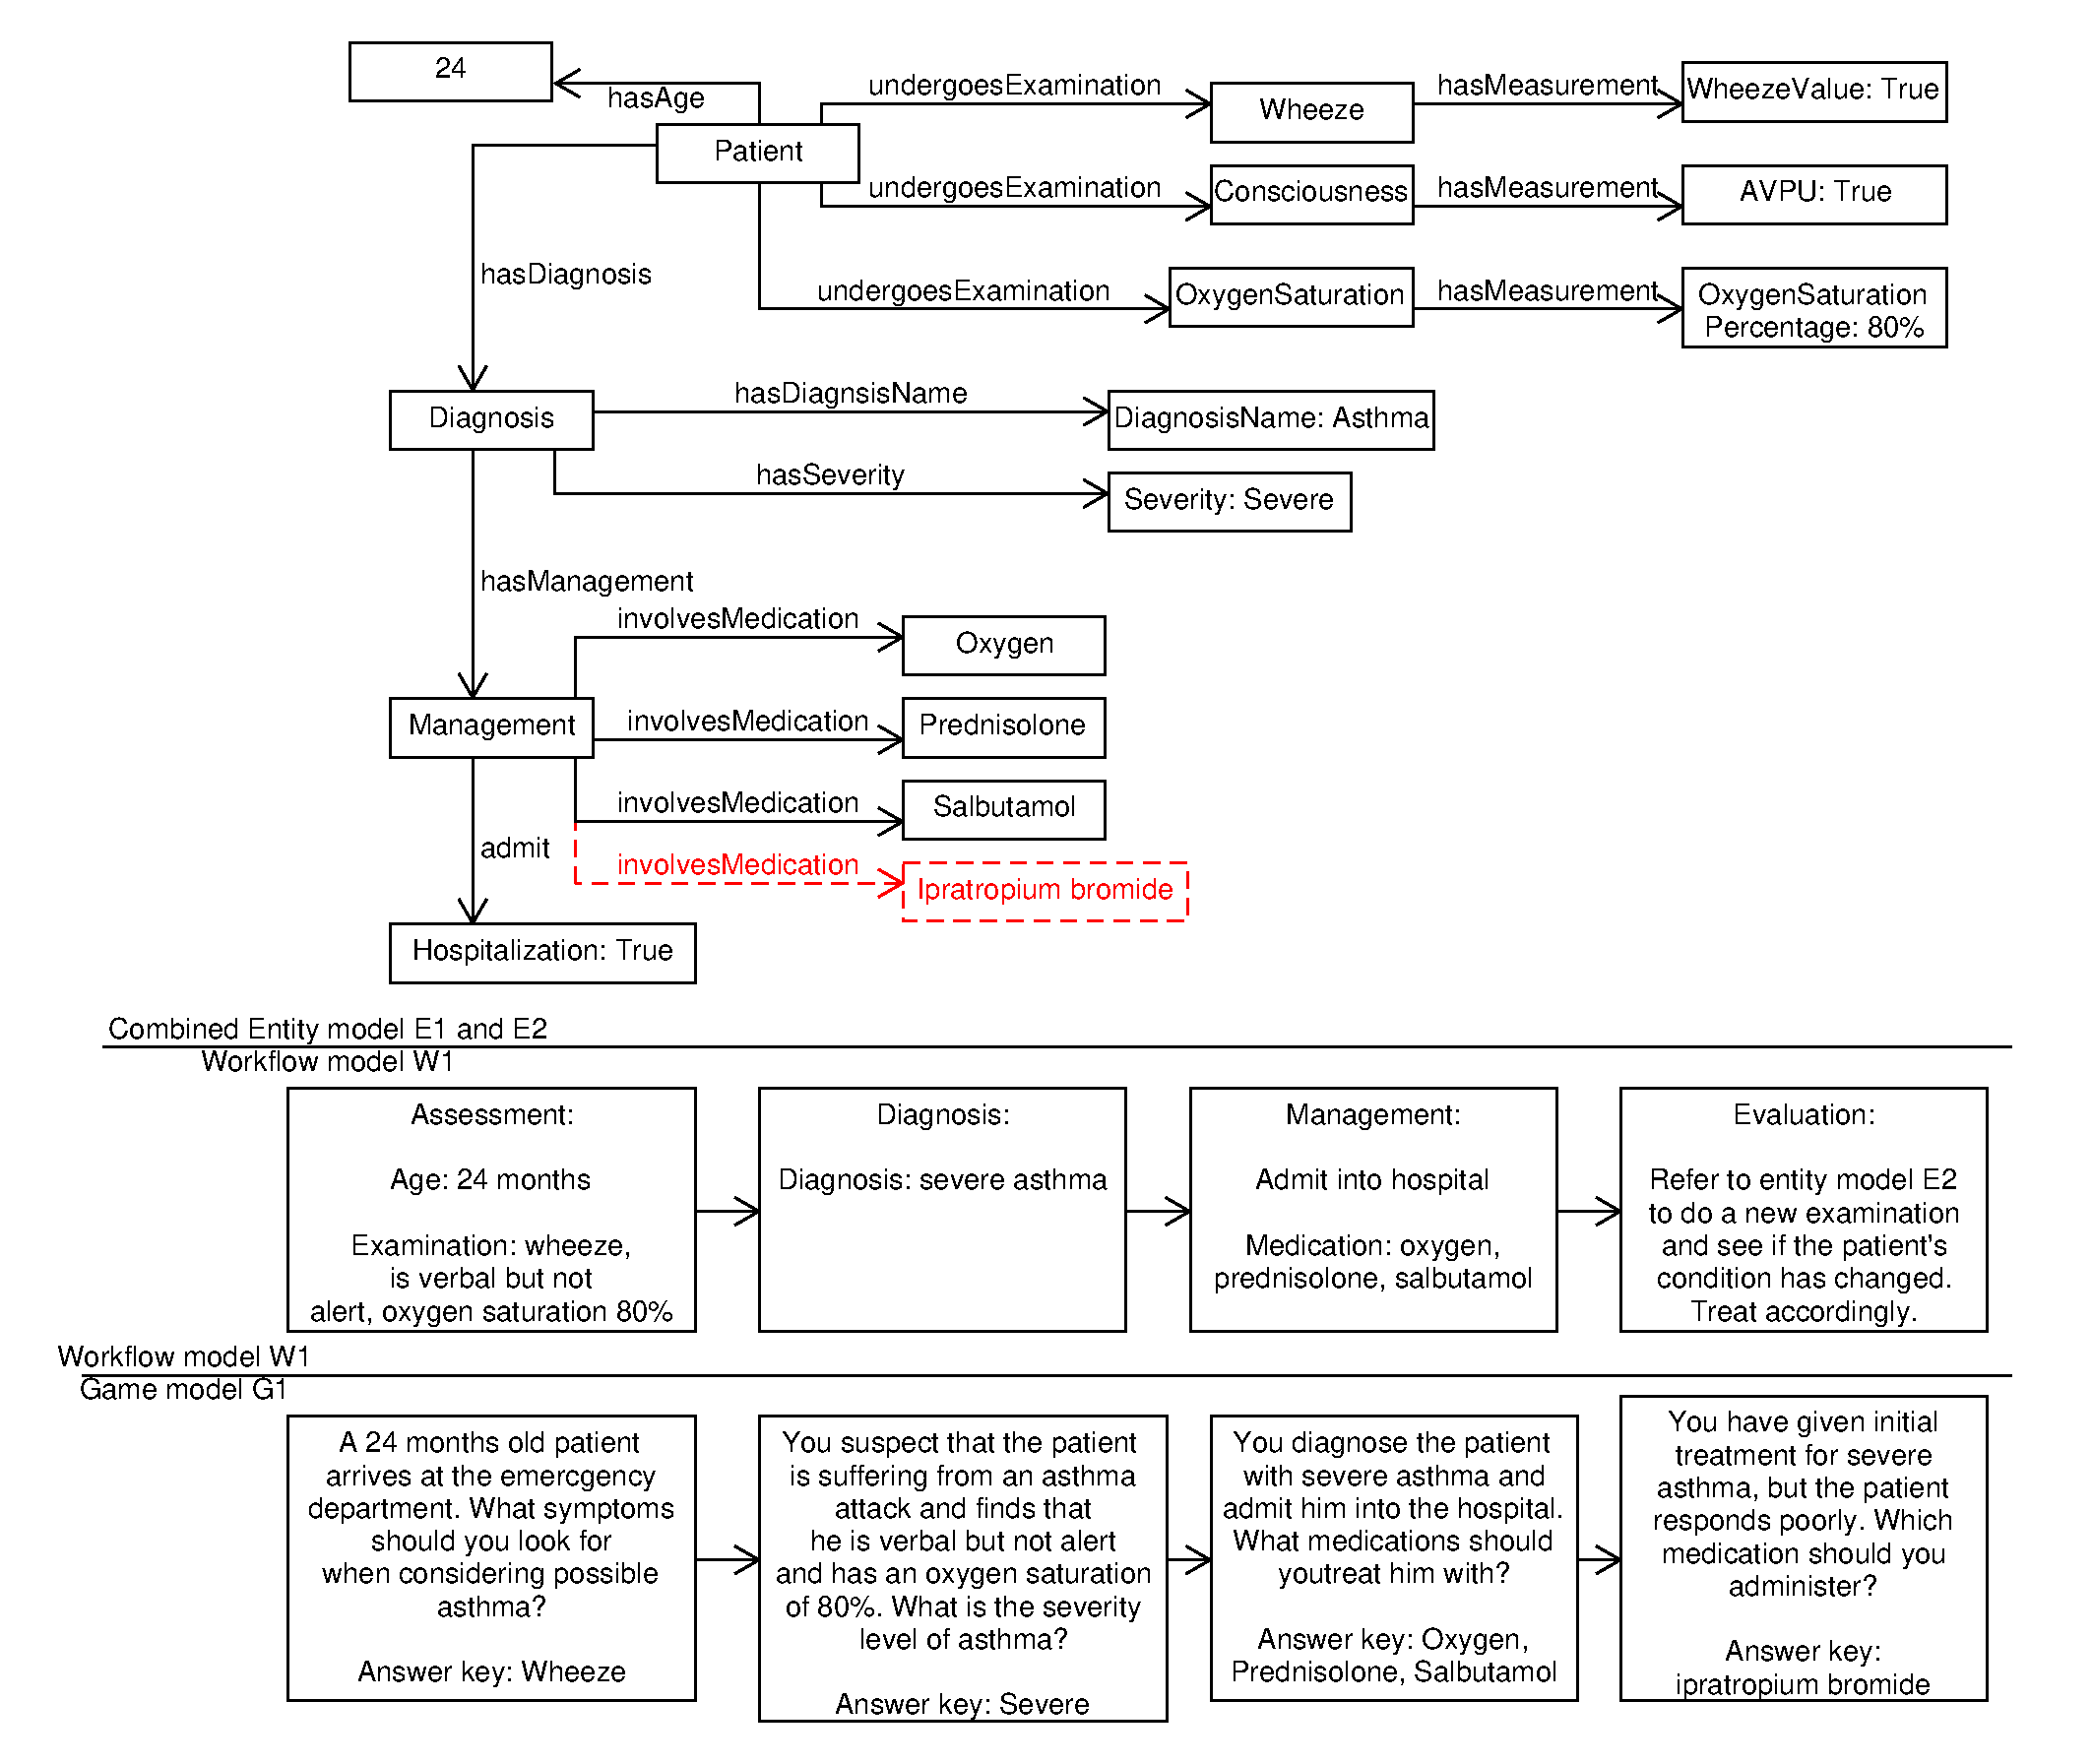
\includegraphics[scale=0.38]{IntegratedEntityGameModels}
	\caption {The entity- workflow- and game models working together to produce a scenario, taking the patient through the steps of a clinical encounter. Note that these are two entity graphs E1 and E2, where E2 gets updated with an additional red vertex Ipratopium bromide. This illustrates a patient which doesn't respond to the initial treatment, and then gets treated with ipratopium bromide}
	\label{fig:IntegratedEntityGamelModels}
\end{figure}

\subsection{Multiple-try feedback}
% https://books.google.no/books?hl=en&lr=&id=GgCPAgAAQBAJ&oi=fnd&pg=PA125&dq=Interactive+with+multiple+tries+&ots=A9Z_BJS5t2&sig=RTv1FmOzU_qic9ADjDgKdJoHamU&redir_esc=y#v=onepage&q=Interactive%20with%20multiple%20tries&f=false
% https://onlinelibrary.wiley.com/doi/full/10.1348/000709905X39134
The quiz uses a concept which is called multiple-try feedback (MTC). That means for every question the student gets more than one attempt to get the answer right. A feedback will be given immediately after each answer is submitted. The feedback consists of a message which tells whether the answer is correct or wrong. If the answer is correct, the user will receive "correct" and an explanation of the answer. If the answer is wrong, there will be no hints or explanations than just "incorrect".

\begin{table}[h!]
\begin{tabular}{ | m{7em} | m{6em}| m{5em} | m{5em} | m{5em} | } 
	\hline
	\textbf{Concept} & \textbf{Abbreviation} & \textbf{Feedback after each question} & \textbf{Multiple attempts at each question} & \textbf{Hints on wrong answer} \\ [0.5ex]
	\hline
No or delayed Feedback & NF or DF & No & No & No  \\
\hline
Knowledge of Correct Response & KCR  & Yes & No & No \\
\hline
Multiple-Try feedback with knowledge of Correct response  & MTC & Yes & Yes & No \\
\hline
Multiple-Try feedback with Hints & MTH & Yes & Yes & Yes \\
\hline
\end{tabular}
\caption{Overview over different quiz concepts}
\end{table}

The point of doing MTC, is to make the student think over what was wrong with his first answer. Did the student misinterpreter the question? Was there a detail he missed? Does the student lack the knowledge or was he just sloppy in his first attempt?

\textcite{Clariana2006} did a study where they divided 82 students into five groups. DF-, KCR, MTC and two control groups. The first control group got a text and a question at the end. The second control group got a text, but there were no question given. After 5 days,post-test was held to see what the students had learned and remembered. The post-test questions were either identical to the questions in the learning material, transposed where the order of the stem of the question and the correct-response gets reversed, paraphrased where post-test questions had the identical content as the learning material, but the phrasing was different and used different words, and a combination of transpose and paraphrasing. The results showed that DF and KCR groups performed better on identical, transposed and paraphrased-transposed questions. MTC performed better on paraphrased questions. The conclusion was that DF and KCR was much better methods for remembering the learning material word for word, but MTC was better when you have to think and reason about what you have learned.

\textcite{Attali2015} further did a did a study on NF, KCR, MTC and MTH using open ended and multiple choice questions on mathematical problems. They showed that solving an open ended question rather than multiple choice was a more efficient way to learn. The learning outcome was the same for the students using NF and KCR. However the learning transfer was greater when using multiple-try (MTC), and even more so when getting a hint on incorrect answer (MTH). They explained the results effortfull and mindful problem solving. In a multiple-try feedback, the user will have to reflect on their errors, re-evaluate the problem and understand the initial error. An open ended question will also require more effort of the student, as they have to generate a an answer rather than selecting from alternatives. On the combination of multiple-try and multiple-choice, it was suggested that some users might be less likely to review their incorrect answer and mindlessly clicking on another alternative. 



According to \textcite{Morrison1995}, students which perform badly on answer until correct questions,  will often become frustrated, loose interest for reviewing the material and probably depress learning.

% From Attali2015, students might assosiate distractions with the scenario in multiple-choice, which is counterproductive when it comes to learning.


As thinking and reasoning about a diagnosis, treatment plan, evaluation and follow-up of a treatment is part of a medical procedure, we believe that multiple-try feedback is the right approach. Because of the nature of a mobile app, where gestures are more convenient than typing sentences, multiple-choice seems to be the right choice even, though open ended questions has proven better results in. There's also a technical problem with evaluating free typed sentences.

Some of the questions in the app are too simple for a hint to be meaningful.Example: "the symptoms for asthma is" and the answer can be "cough and wheeze". Where hinting "cough", would be giving away the answer, especially in a multiple-choice format. However, the data model supports hints as links to external learning material. E.g. the student could look for the answer in the guideline itself.

We solved the "answer until correct"-problem described by \textcite{Morrison1995}, by having a "read more" button displayed upon incorrect answer. The "read more"-button will display the correct answer, an explanation and continue to the next question. Avoiding the user becoming frustrated and discouraged by having to brute-force the answer keys to progress.




\subsection{Reward system}
% SHOW ANSWER
By having multiple-try feedback, another problem rises, and that is the reward system. If there is no penalty for incorrect answers, a student which needs ten attempts per questions, will get the same score as a student which answers all the questions correctly on the first attempt.

\textcite{Attali2015} solved the problem by giving 1 point for answering correctly on the first attempt. 2/3 points for the second attempt, 1/3 for the third and 0 points if the third attempt was incorrect. A limitation with this method is that it makes no sense for the student to make more than three attempts. \textcite{Morrison1995} had another strategy where they adjust the scores by dividing the total score by the total number of attempts during the quiz. A consequence is that attempt number two will have a huge penalty which is halving the students total score. While attempt number twenty will give a very small penalty from attempt nineteen. A method to dampen this effect could be dividing the total score by the sum of reviews and number of questions. Another method could be taken the square root of the question reward for every attempt the student has on that question.

The solution we used was having a fixed value for every answer alternative. The quiz author chooses the penalty for each distraction and reward for each answer key. The idea is that the distractions can have some sort of degree of wrong or right, and this can be reflected in the scoring. On the question "what are the symptoms of asthma?", "difficulty breathing" is a more correct answer than "fever", as "difficulty breathing" is a symptom of asthma in combination with wheeze. Fever is not an asthma symptom at all. In future work, the penalties can be automated as you can see from the entity model whether the symptom belongs to the asthma guideline or not. A distraction from respiratory disorders may give a larger penalty than a distraction from the asthma guideline, but smaller penalty than symptoms not belonging to respiratory diseases.

Both \textcite{Attali2015} and \textcite{Morrison1995} avoids the scenario where the user gets a total minus score. This may be a strength of these methods, as a negative total score seems like a very harsh feedback and might demotivate the student. In our solution we use negative numbers as penalties on distractions, such that a negative total score may happen. We try to limit the likelihood of a negative score by providing a very high reward for a correct answer and a very small penalty for a distraction. Typically the reward is 10 points and the penalty -1 og -2 points. The intention is to encourage the student to review the incorrect answer and try again. As the format is multiple-choice and the penalty-reward ratio, there is a little risk involved trying multiple times. But giving up by clicking "learn more", the student will not get an additional penalty, but will miss out on the reward. By clicking answer alternatives mindlessly and consequently clicking "learn more" will probably not end up in a negative score, but is more likely to end up in a negative score than mindlessly click answer alternatives until correct.

%----------------------------------------------------------------------------------


%Each question will have several answer alternatives the student can choose from. Each answer alternative will have a reward or penalty related to them. The correct answer will have a great reward, while wrong answers will have a small penalty. The quiz author will have the opportunity to specify the rewards, such that he can give even smaller penalties for partly correct answers. The idea of the reward- penalty system is to increase learning. if the student answers wrong the first time, he will be given the possibility to reflect over the question once more or perhaps read the guideline to learn before he commits his second attempt. We are aware that providing a minus score for making an attempt can be very demotivating, but it is to avoid the situation where a student gets the same (or better) score for making ten attempts than only needing one attempt. A small penalty will have a very small impact when the reward per question is high, but in situations where the student performs very poorly and ends with a negative total score, it is possible to adjust this to a small positive score on presentation for the student. Not giving a too harsh feedback for trying to learn.



%\textcolor{red}{A solution to having a not very strict game, encouraging to playing and learning, one can also have a very strict examination version. The idea is that after examination, the results will be sent to the lecturer (or a governing body of some kind) to evaluate what the overall knowledge of the students, as well as details of what the students are really good in and where do they struggle. The lecturer can then target the weak of points of the students in one of the next lectures. }




\section{User manager}
The user manager stores the scores of previously played quizzes on the student's game. By fetching the last played game for a specific quiz, it knows the student's current knowledge level. The stored scores represents the student map, and also shows the student's current position in the learning map. By analyzing the student map, we can see the student's progressions.

The user manager will also keep track of the scores during a quiz game. At the end of the game, the user can be notified if he got demoted to an easier level, promoted to play more difficult content or show the student how close he is to complete the current difficulty level.

\subsection{Visualization of game statistics}
The student needs some feedback, where he is in the learning map, how close he is to pass an evaluation, how close he is to progress to the next level and in the case where he gets relegated to an easier difficulty level.

The scores for the evaluations can be shown as bars in a graph, and the passing conditions as a line. When the bars reaches or passes the line, the student knows that the he has met the passing condition for the evaluation at that level. This can also work as a motivation for the student, as he sees that he gets closer and closer to the passing condition as he learns he more and performs better.

To visualizing where the student is in the learning map, has been solved by showing the learning map in almost a table format. Colour combinations shows which evaluations have been unlocked, which are locked and which are the current ones the student plays. Red and green indicates whether a student gets relegated from a level or whether he progresses to the next level.


\section{Conceptual model of how all the classes are connected in Game Engine}
The conceptual model of the game engine is shown in figure \ref{fig:ConceptualGameElements}. Category is a quiz game for a certain CPG, such as the paediatric possible asthma guideline \parencite{RepublicofKeny2016}. Each of these quiz categories are divided into several disciplines. Disciplines are themes in knowledge units, which we identified using DCM (dynamic content management). Each of these knowledge units contain evaluations at different difficulty levels. These evaluations are collections of questions, which contain a collection of multiple choice questions and answer elements.

The quiz data are read from JSON-files, which are produced by a content author. The quiz author defines a quiz for a specific CPG. He identifies themes for content units, which contains evaluations with varying difficulty levels. The questions are written in a template format, which we have already covered. The templates contain tags, which refer to vertices in the entity graph, representing a given patient. The answer key is also such a tag, referring to one or more vertices in the entity graph. When the quiz is initialized, the tags will be replaced with values from the entity graph. The content author will write answer alternatives for each question, where he specifies a reward (or penalty) for each of the answer alternatives. An answer alternative which matches the answer key value in the entity graph will represent the correct answer. The content author needs to know what is in the entity graph to be able to provide meaningful rewards.

The student skills is the scores from the last played game, and is fetched from the database on the student's phone. The allowed- and unallowed levels are calculated from the student skills and the requiredMinSkill for each level. Unallowed levels are levels that the student can't play and are locked for the student, as the student's score is lower than the required minimum skill.

A new instance of skill will be created when the student starts a new game. This instance will hold the scores for the current game, and will be stored to the phone's database once the game has been completed. This score determines which levels the student can play in the next game of this category.


\begin{figure}[h!]
	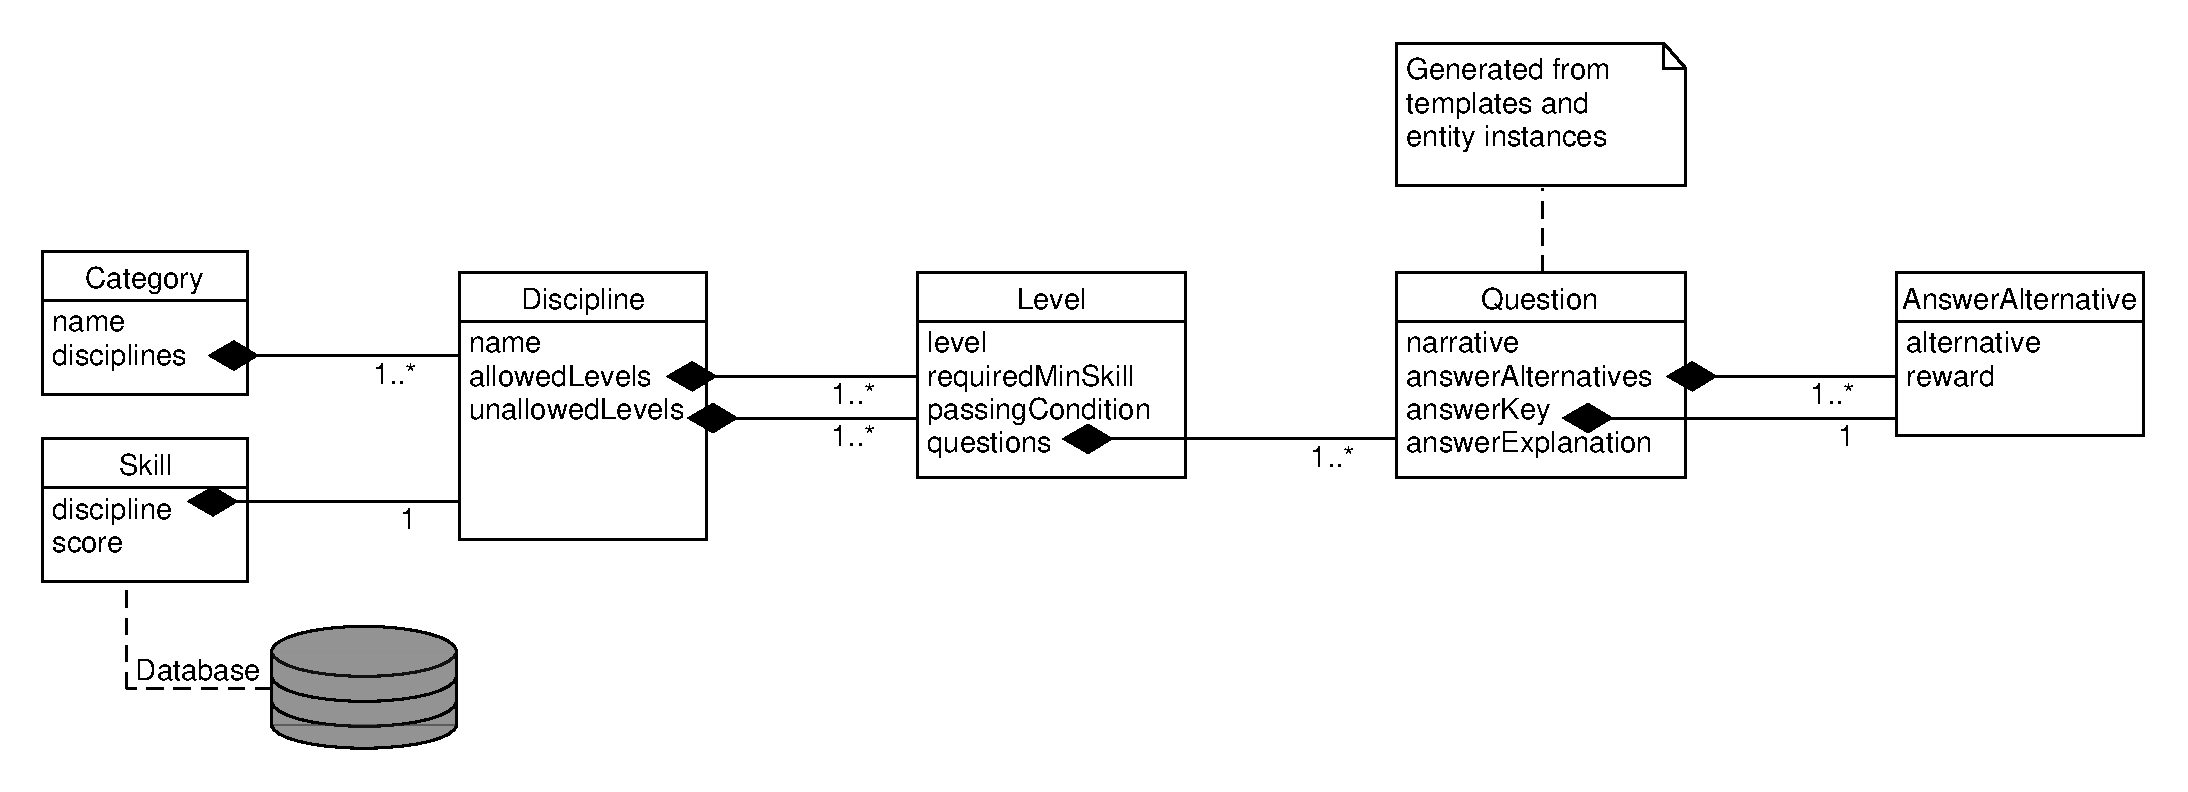
\includegraphics[scale=0.36]{ConceptualModelGameElements}
	\caption {Conceptual model for the game elements}
	\label{fig:ConceptualGameElements}
\end{figure}

One problem with the conceptual model is that it is somewhat complex. Once we have determined which levels we should pick questions from and we have generated the questions, we really don't need the structure. Especially when playing scenarios, it is nice to just go through an ordered array, instead of dealing with "now I've played the third question of level 2 diagnosis, the next question in this scenario is the third question in level 2 management, unless I've already completed level 2 management in the previous run of the game. Then the next question is follow-up instead". We rather deal with the problem at the initialization phase and just go through the array when playing the game. A solutions is to implement the façade pattern \parencite{Gamma1994}, such that other parts of the system can use the game engine, without having to deal with the underlying complexity. 

% Not sure whether this is facade or mediator pattern thouh

\begin{figure}[h!]
	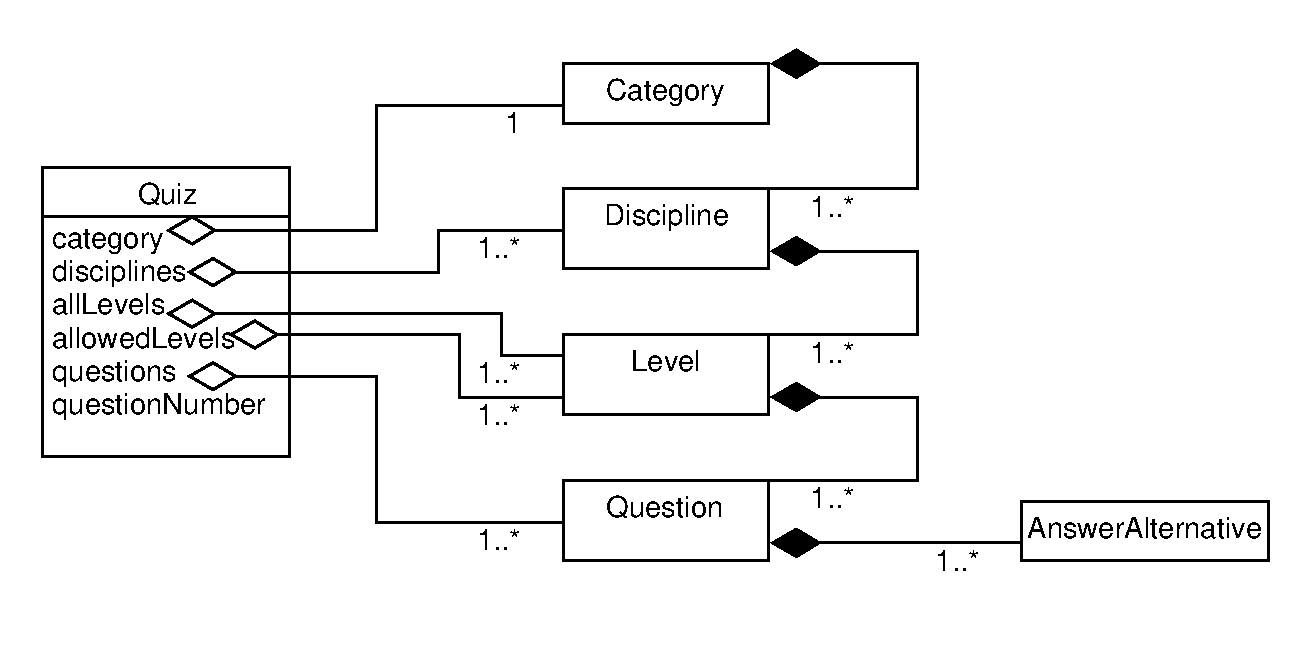
\includegraphics[scale=0.4]{GameEngineFacadePattern}
	\caption {Façade pattern hides the complexity of the game engine and makes it easier for other parts of the system to use it}
	\label{fig:GameEngineFacadePattern}
\end{figure}

%\textcolor{red}{Should I show how I populate the models with data from JSON and database? I'm not very happy about the code on that part.}
% DON'T KNOW IF I SHOULD SHOW THE GAME ENGINE PACKAGE HOW TO POPULATE THE MODELS AS THIS CONTAINS HARDCODED AND NASTY STUFF TO GET PROGRESS QUIKLY

%\begin{itemize}
%	\item DAO
%	\item Models
%	\item Templates/Narratives/AnswerKey
%	\item Quiz is kind of an interface
%\end{itemize}




 

\section{Summary}
The chapter is structured after the conceptual training managers in the game engine. Question flow manager, conversation manager and the user manager.

The question flow manager uses the Dynamic Content Manager (DCM) to make the questions adaptable to the student's knowledge level and flexible such that the student can choose his own path through the learning content. We used the workflow model as a base, to categorize the learning material, and we identified knowledge dependencies between them, making a knowledge map. We saw how we could make three difficulty levels by adjusting the detail level of the questions, by going from factual questions, to scenarios and then detailed scenarios. 

The conversation manager made textual questions by using instances of the entity model and templates. Tags in the template pointed to vertices in the entity model, such that we could produce many questions with one template, pairing it with different instances of the entity model. However, the entity model had to be expanded with presentation vertices as the data types couldn't be directly parsed into a textual presentation. 

Further we argued why we wanted to use multiple-try questions with feedback. The student can try as many times as he wants to get the answer correct. The idea is that the student has to revise the question and reflect on why the question was wrong and how can he correct it. We also described the reward system, which will fit the multiple-try approach. A student with ten attempts should get a lower score than a student which answers correctly on the first attempt.

We then described a conceptual and technical model of how all the classes are connected in the game engine.





\chapter{Application Walkthrough}
\section{The mobile application}
\begin{itemize}
	\item React
	\item React-Native
	\item React-Native-Navigation (Wix)
	\item Redux
	\item React-Redux
	\item Redux-Thunk
	\item Highcharts
	\item Jest
\end{itemize}
\subsection{React-Native and Redux}
\subsection{User interface and flow of the user interaction}

We will now go through the application, by playing a level 2 scenario. We will discuss the game elements, the user interface, the technologies which are used. Whenever it is necessary to clarify we will also go deeper into the implementation.

The application is written in JavaScript, using the mobile application framework React Native \parencite{ReactNative}. The intention of using such a framework, is in the future to make iOS and UWP versions, without having to rewrite the entire application. As React Native uses the React web framework \parencite{React}, JavaScript, and that we can decouple some of the data management logic through Redux \parencite{Redux}, allows us to reuse a lot of the code if we later want to make a web version at a later point.

When the student first starts the application, he will presented with the screen in figure \ref{fig:ScreenshotMain}. The Game Engine will keep track of which quizzes we have installed, and displays them here. At a later point we can make knowledge dependencies, where a user have to complete basic courses like prescribing oxygen \parencite{RepublicofKeny2016} and antibiotics administration \parencite{RepublicofKeny2016}, before the paediatric possible asthma guideline \parencite{RepublicofKeny2016} can be played. This is theory from Dynamic Content Management \parencite{Eide2008}.
\begin{figure}[h!]
	\caption {The entry screen where the student can choose between playing different quiz categories}
	\label{fig:ScreenshotMain}
	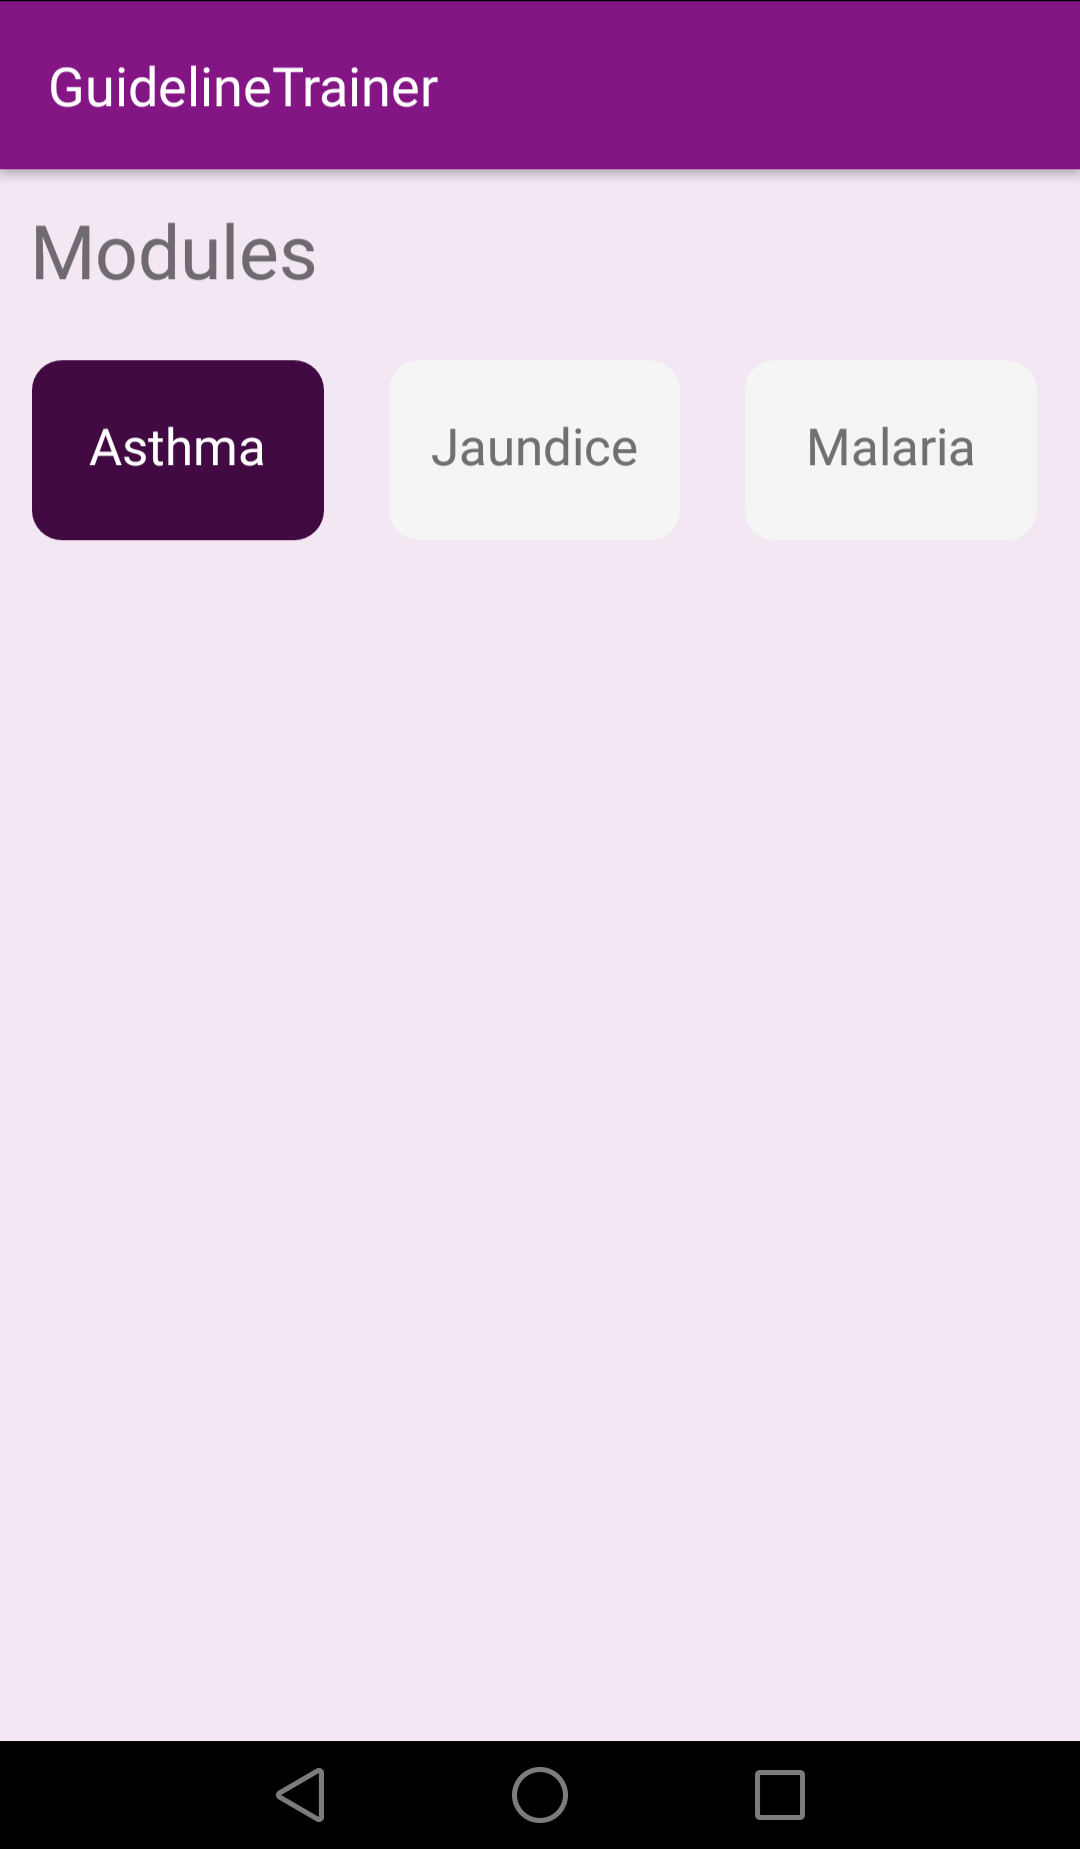
\includegraphics[scale=0.2]{ScreenshotMain}
\end{figure}

In \ref{fig:ScreenshotLearningMap} we get presented with the learning map from Dynamic Content Management \parencite{Eide2008}, and the student's position in the learning map. The boxes with the green background indicates the student's current position and which levels he will get questions from. The other background colours indicates which levels have been completed and which levels are uncompleted and locked. 

The student's position in the learning map is fetched from the database on the student's phone, and gets updated every time the student completes a quiz for this category. The database calls are asynchronously and loosely coupled using redux thunk \parencite{ReduxJS-thunk}, such that the web version would replace the database related functions with fetch related functions to for example do REST calls to a REST service. 

In the header we see a back arrow. This is React Native Navigation \parencite{Wix} which handles the navigation in the application, which makes it possible to click the arrow to go back and choose another quiz to play instead. This fulfils "Provide Clearly Marked Exits", which is one of the usability heuristics for user interface design given by Jakob Nielsen and Rolv Molich \parencite{Molich1990}.

\begin{figure}[h!]
	\caption {The student is shown his position in the learning map. Completed, active and locked levels have all different colours}
	\label{fig:ScreenshotLearningMap}
	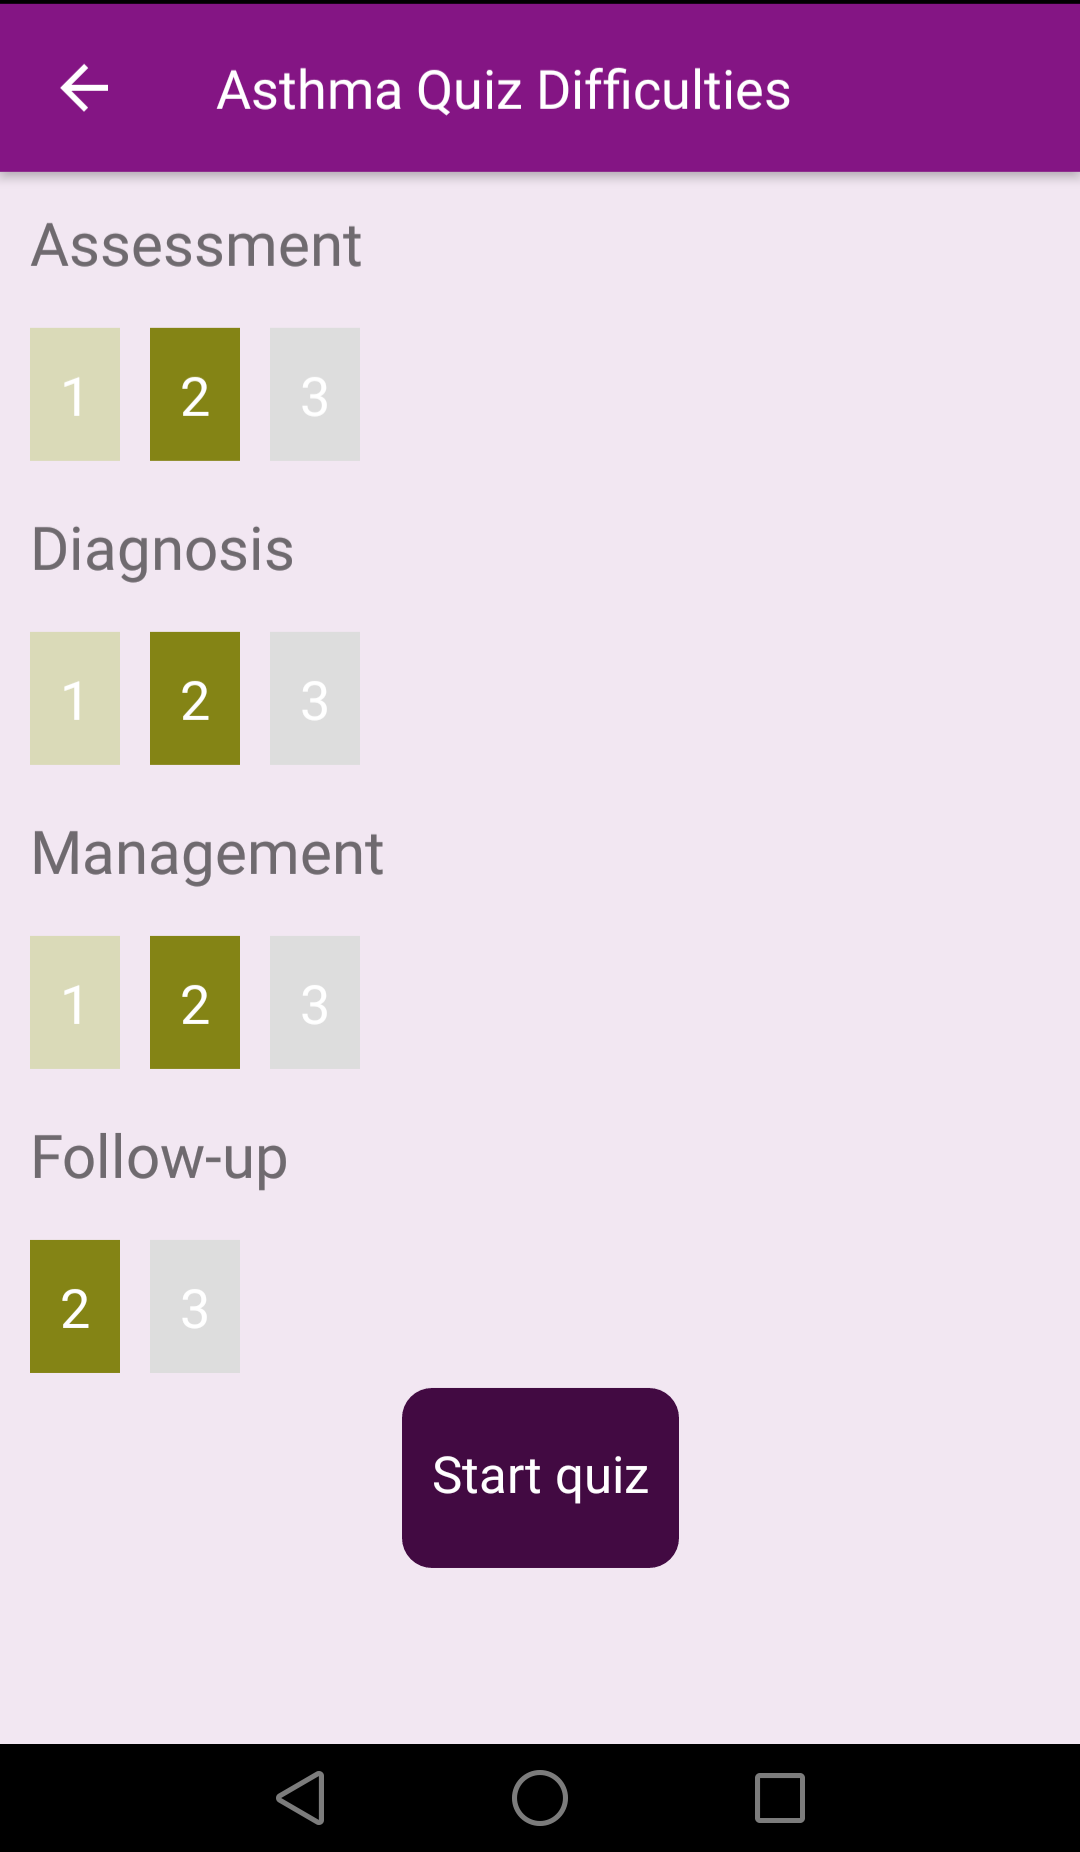
\includegraphics[scale=0.2]{ScreenshotLearningMap}
\end{figure}

In \ref{fig:ScreenshotKarenAssessment} we are presented with a multiple choice question. The question is in the form of a scenario, where we go through the workflow model, where the first step is the assessment.  

The Game Engine holds a template and a reference to the entity instance graph which is being used with this template. The template contains tags which refers to vertices in the entity graph. The entity instance graph holds textual presentation of each vertex which is being printed into the template, which results in a neat and coherent text. 

The Game Engine an answer key, which is a tag pointing to one or more vertices in the entity instances. The Game Engine also holds hard coded distractions, where one of them matches the vertex/vertices which the answer key points to. Points and penalties are specified for each of the distractions in the Game Engine.

Here the student answers correctly, is awarded points and is being presented with an answer key explanation. The Game Engine holds the answer key explanation together with the question. 

The student can click on "next" any time he is ready to proceed to the next question.
\begin{figure}[h!]
	\caption {The first question is an assessment question. Here answered correctly and an answer key explanation is given}
	\label{fig:ScreenshotKarenAssessment}
	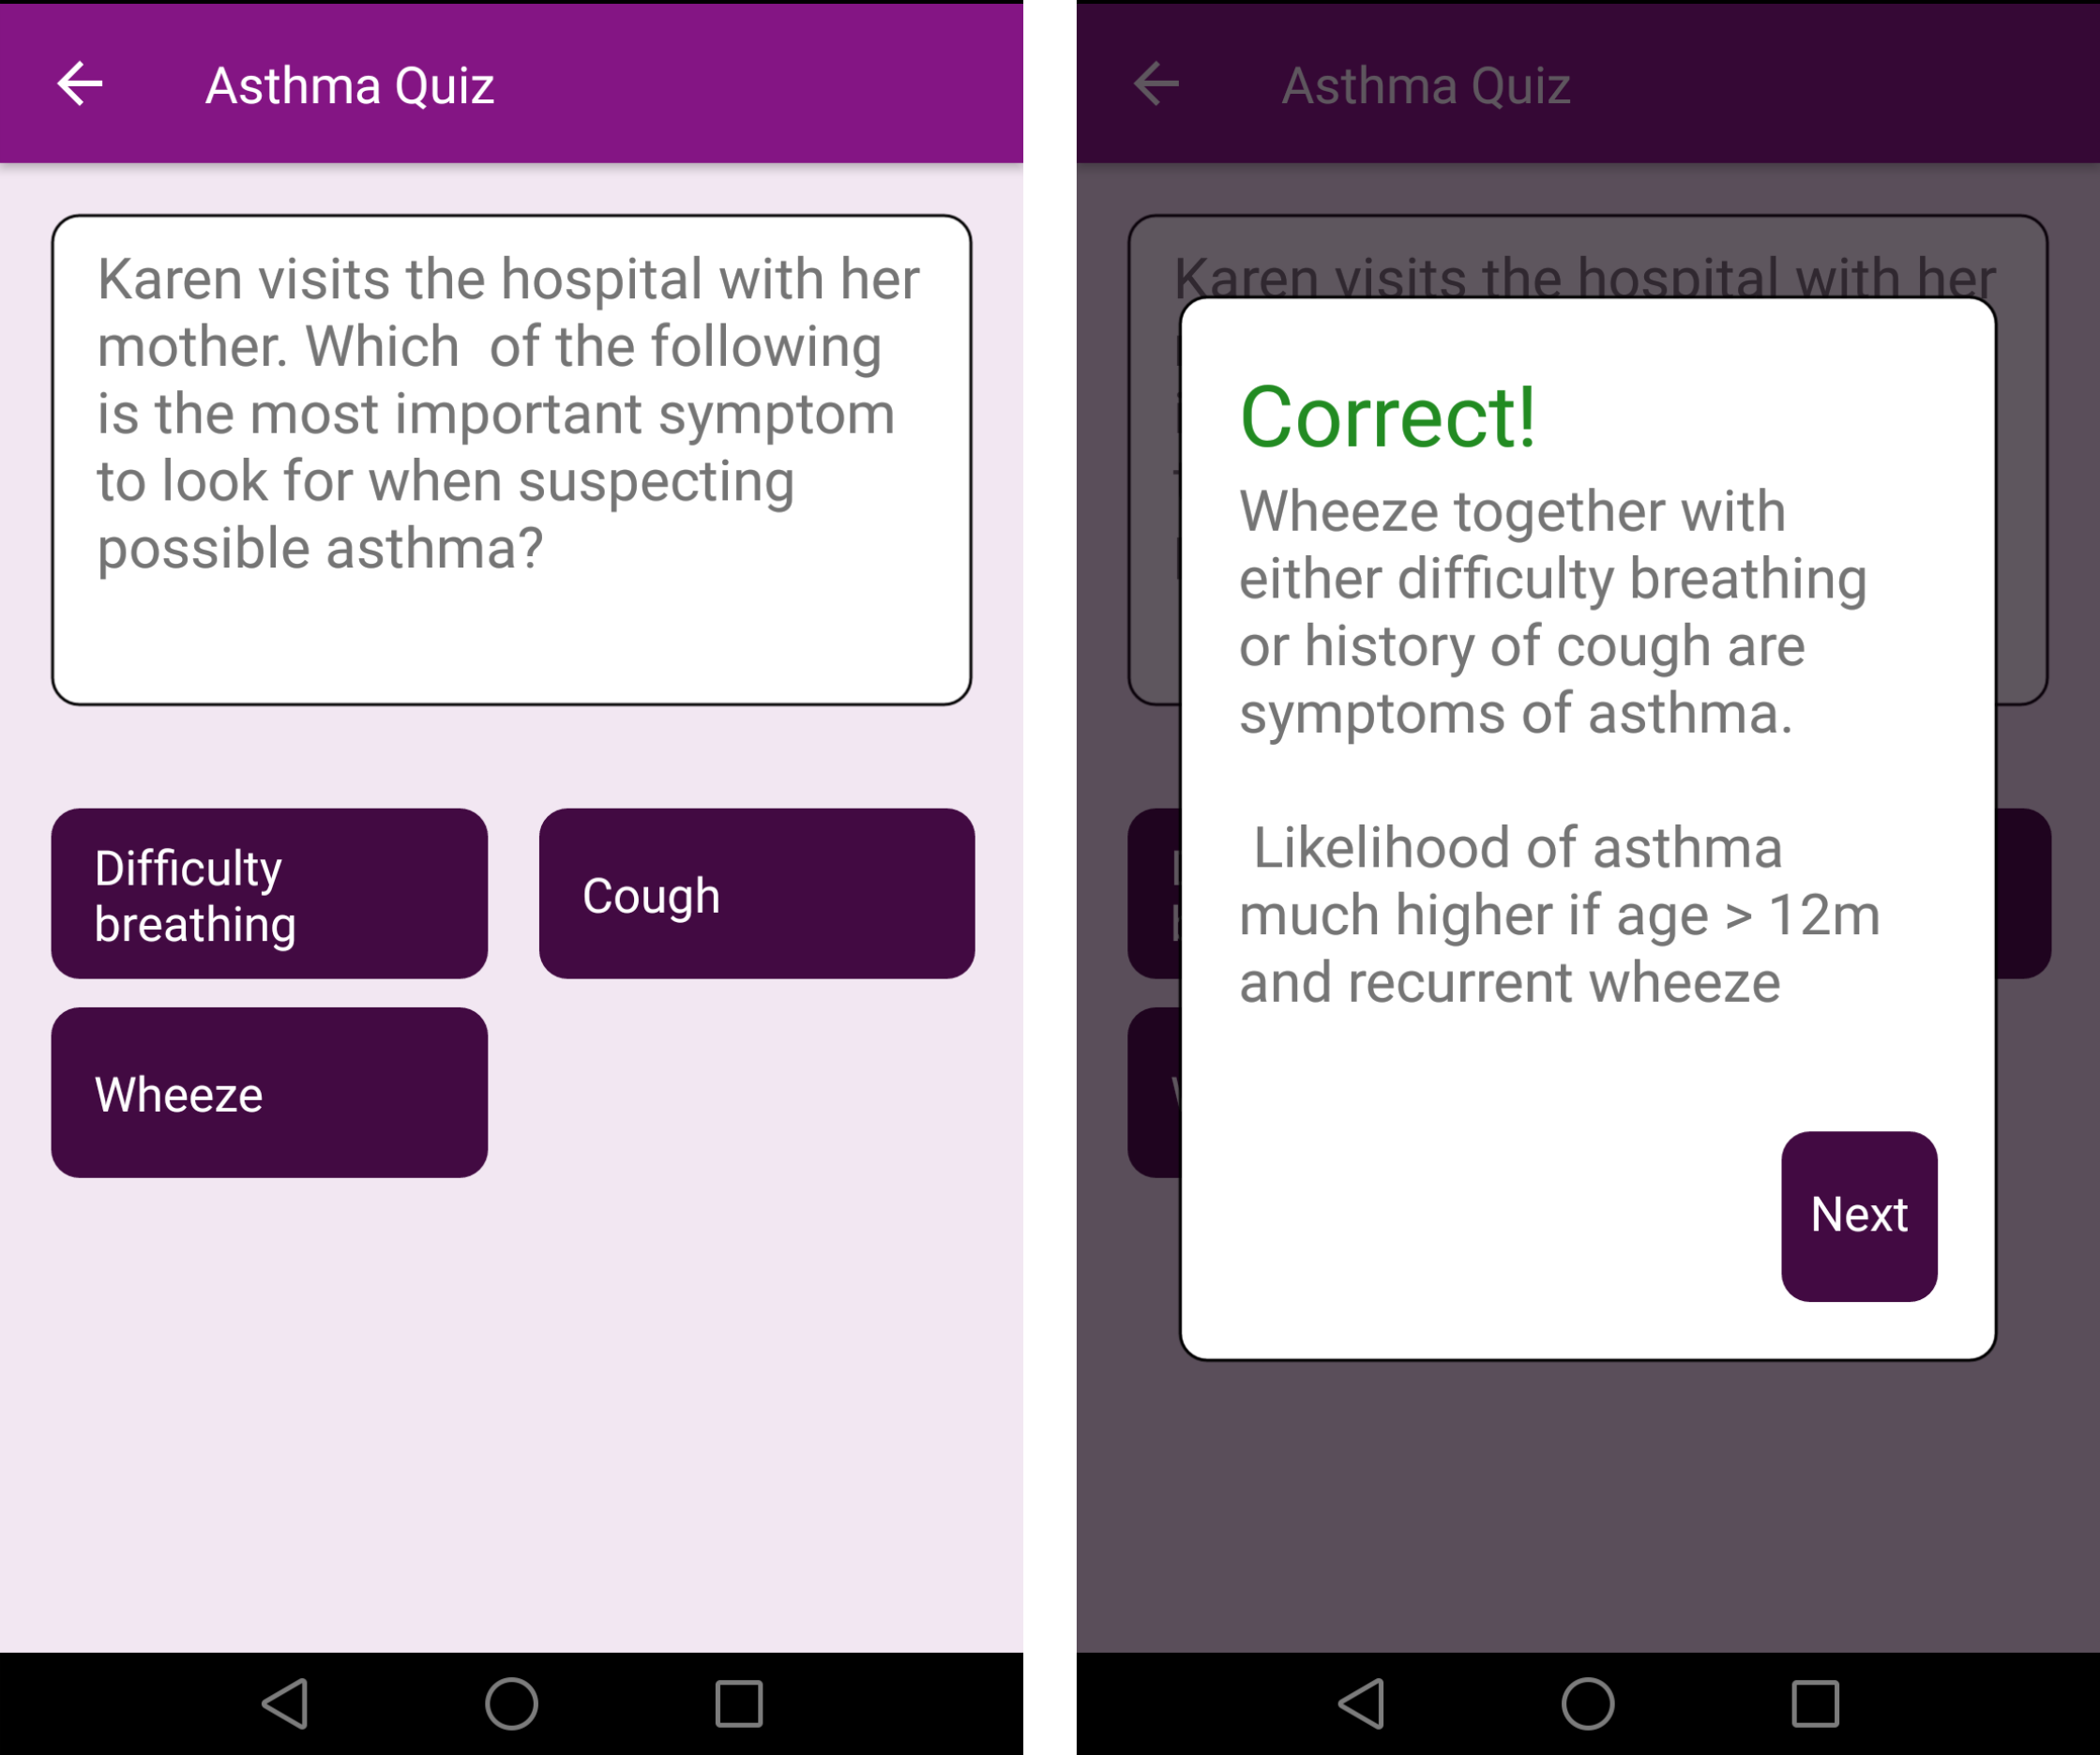
\includegraphics[scale=0.2]{ScreenshotKarenAssessment}
\end{figure}

In figure \ref{fig:ScreenshotKarenDiagnosis} we continue to the next step in the workflow model, the diagnosis. Here the student will be provided with symptoms which will determine the severity of the asthma.
\begin{figure}[h!]
	\caption {The second question is for diagnosis}
	\label{fig:ScreenshotKarenDiagnosis}
	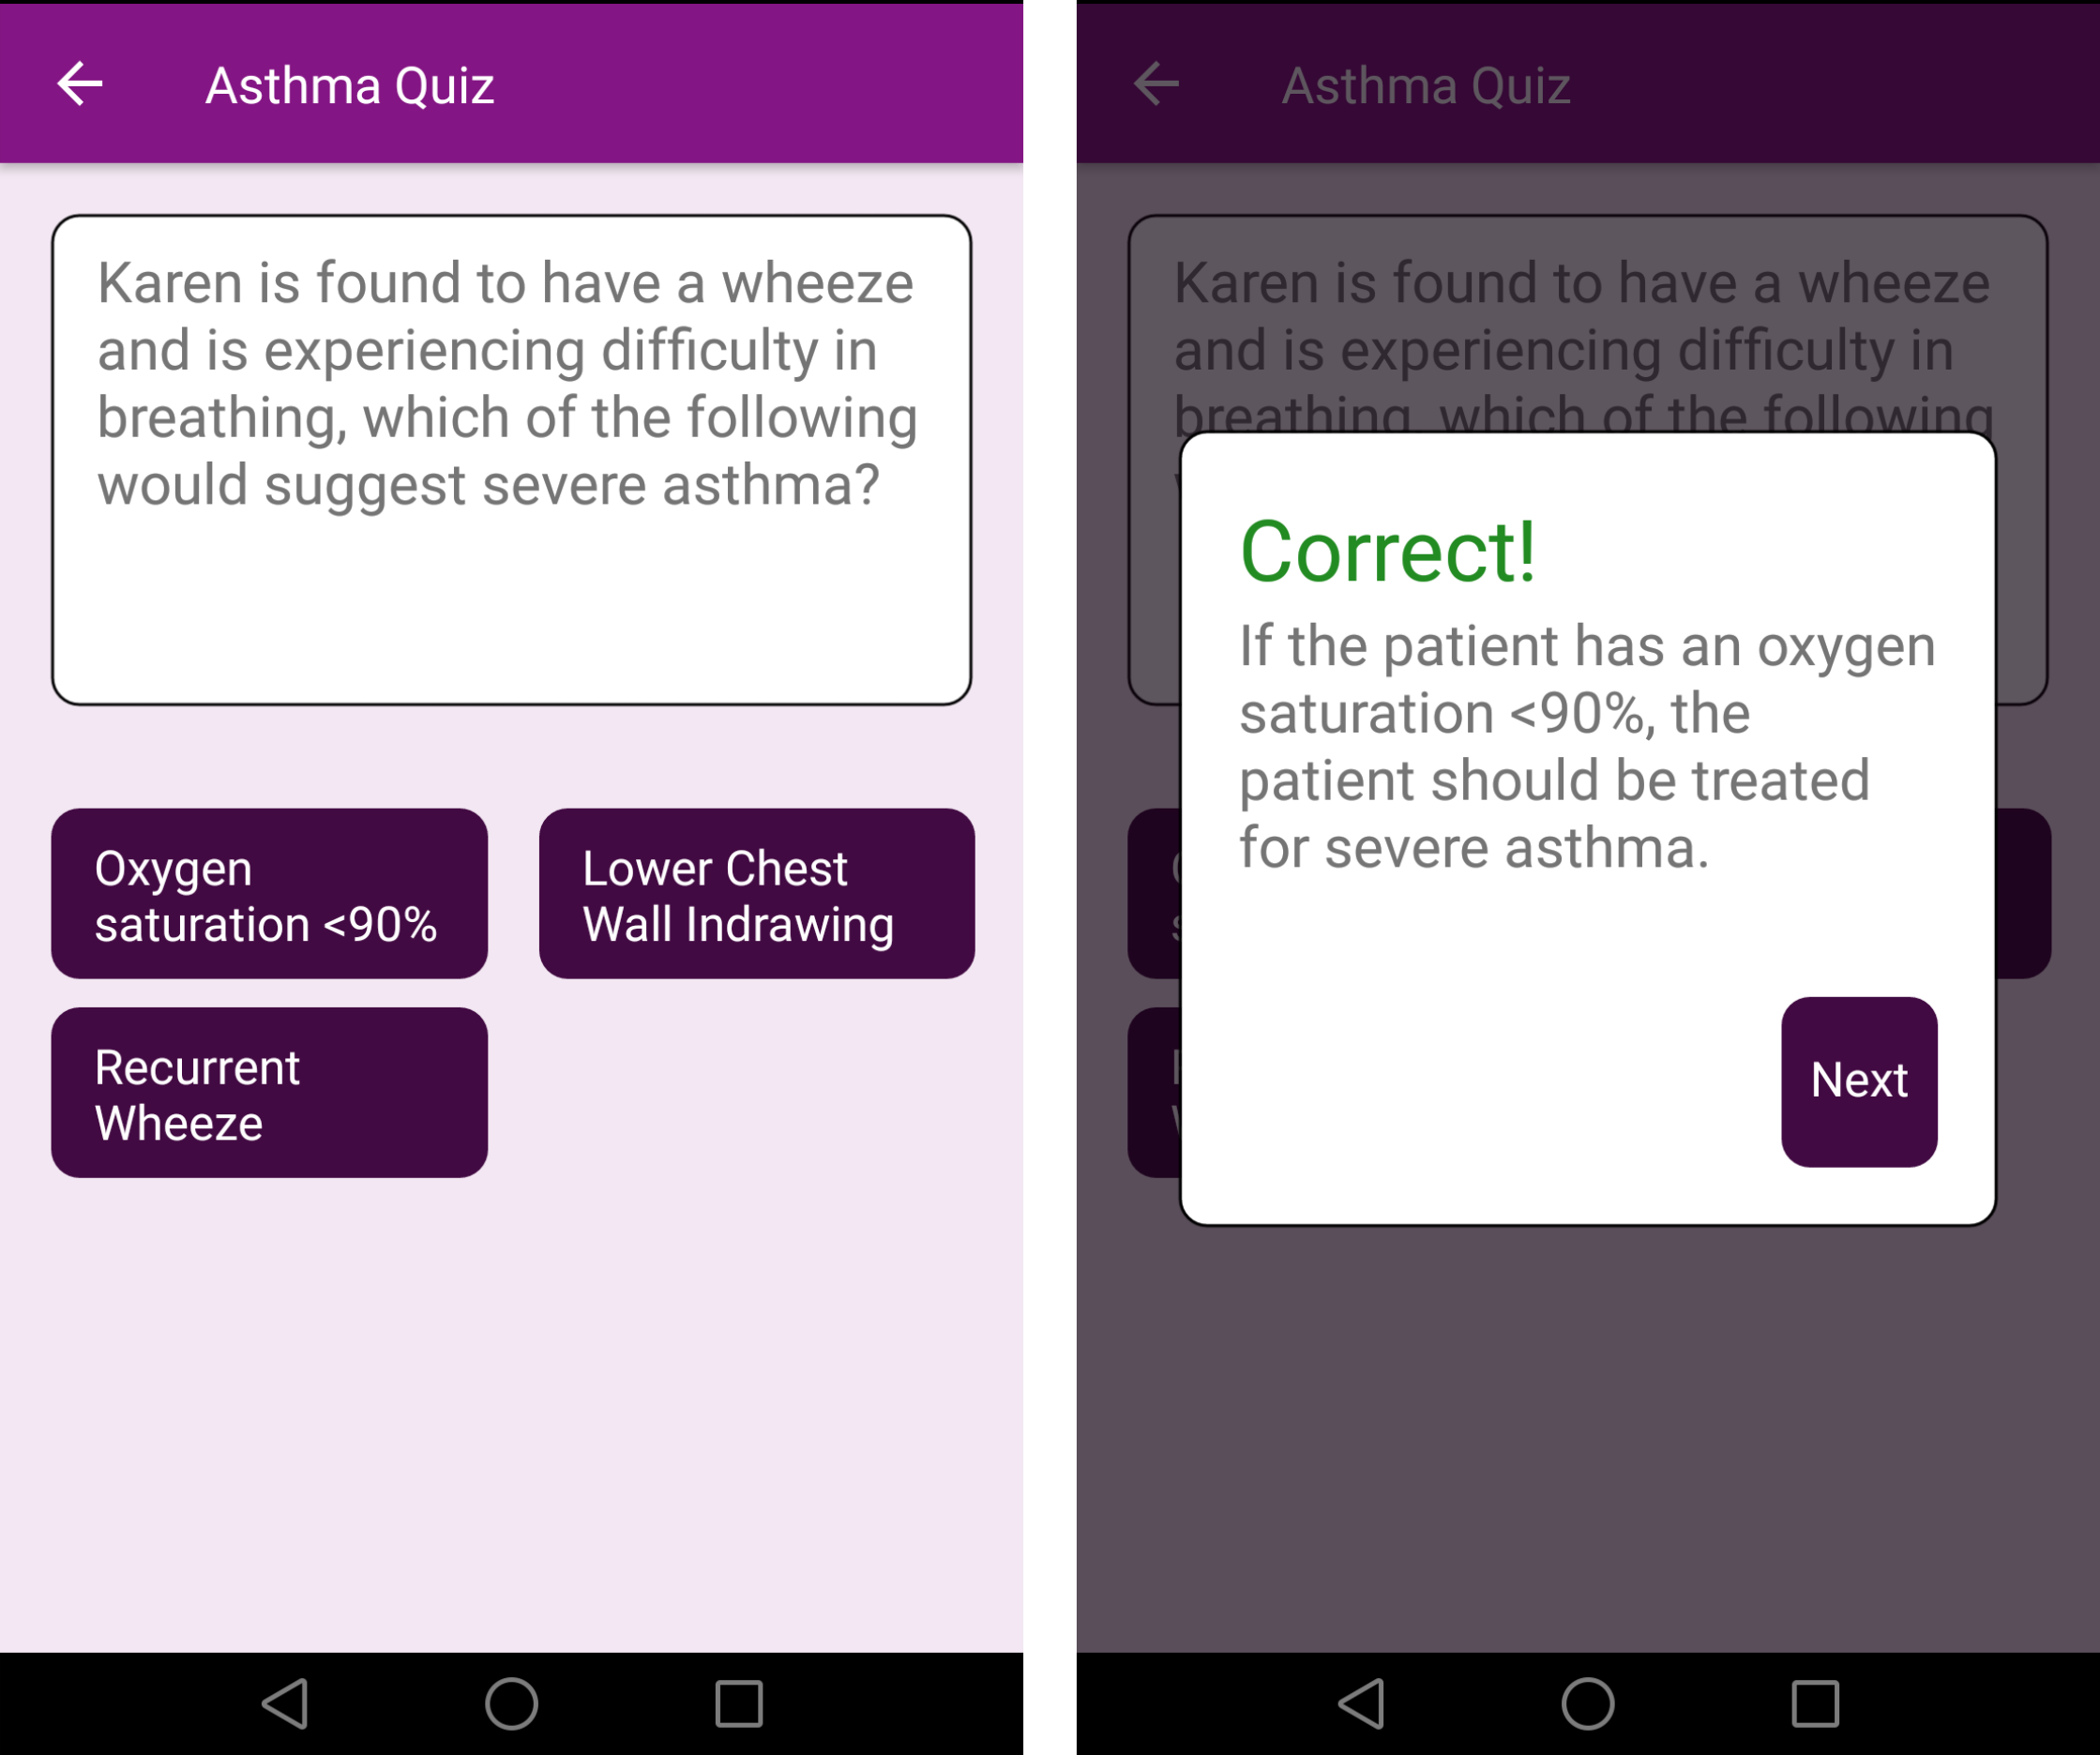
\includegraphics[scale=0.2]{ScreenshotKarenDiagnosis}
\end{figure}

In figure \ref{fig:ScreenshotKarenManagement}, the student gets a question from the management part of the workflow model. Management can be admitting the patient to the hospital, medication administration or advise.
\begin{figure}[h!]
	\caption {Third question is for management}
	\label{fig:ScreenshotKarenManagement}
	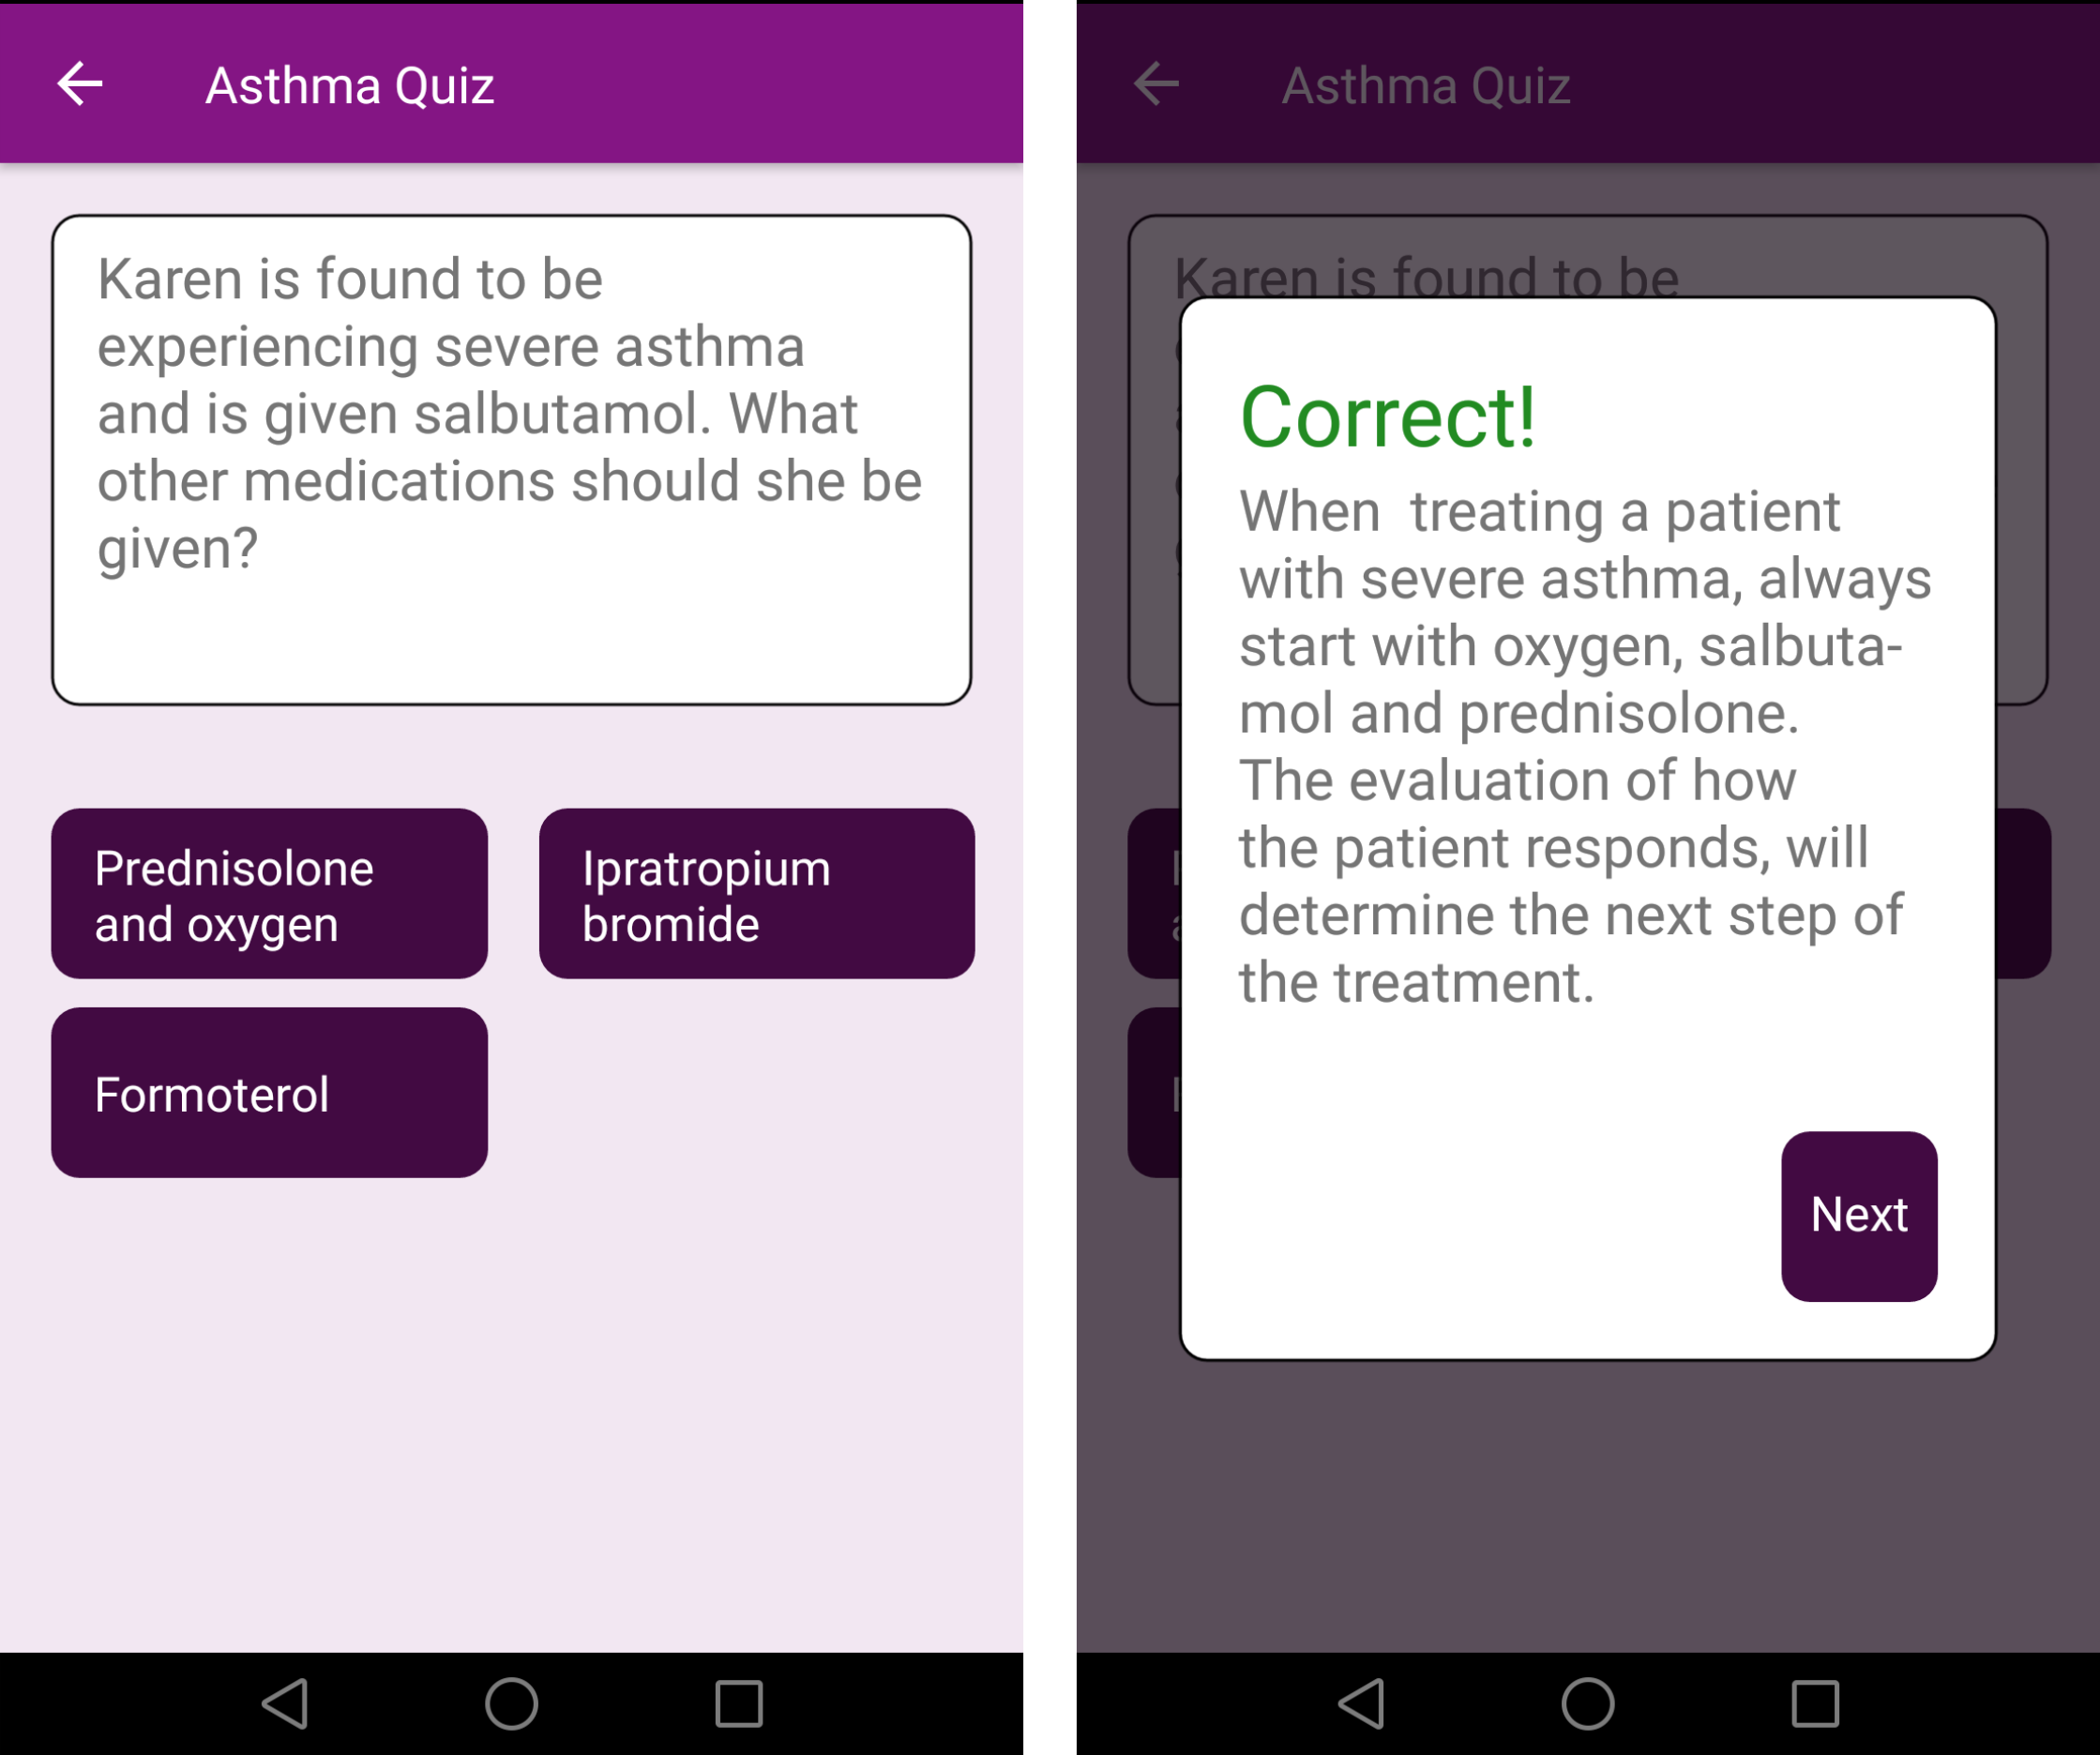
\includegraphics[scale=0.2]{ScreenshotKarenManagement}
\end{figure}

In figure \ref{fig:ScreenshotKarenFollowUp}, the patient has been through the initial treatment, and the student is asked on how to follow up the patient. Here the textbox in the screenshot is a bit small for the text, but the student has the possibility to scroll inside the textbox. The question is what is the maximum of days the patient can be on prednisolone.

Initially the student picks the wrong answer. The application displays a hint and a feedback, telling the student that this answer was wrong. The student is awarded with a penalty in points. As no further information is given rather than that the previous answer was wrong, the student is given the possibility to try again. If the student tries again, a wrong answer will give a further penalty. We have made sure that the penalty is much smaller than the reward, typically 10-20\% of the reward, trying to motivate the student to revise his answer. The student can try as many times that he would like, to get the answer correctly and collect the reward.

As we don't want to force the student to retry until correct, we have the option "learn more". When the student clicks on this button, he will be presented with the answer key explanation as well as the option to proceed to the next question. When the student decides to click on "learn more", he will miss out on the reward.
\begin{figure}[h!]
	\caption {The fourth question is follow up. We answer incorrectly the first time. The answer key explanation is not shown, and we can choose to revise the question by clicking "try again". If we press "learn more", the answer key explanation is instead shown, and we continue to the next question}
	\label{fig:ScreenshotKarenFollowUp}
	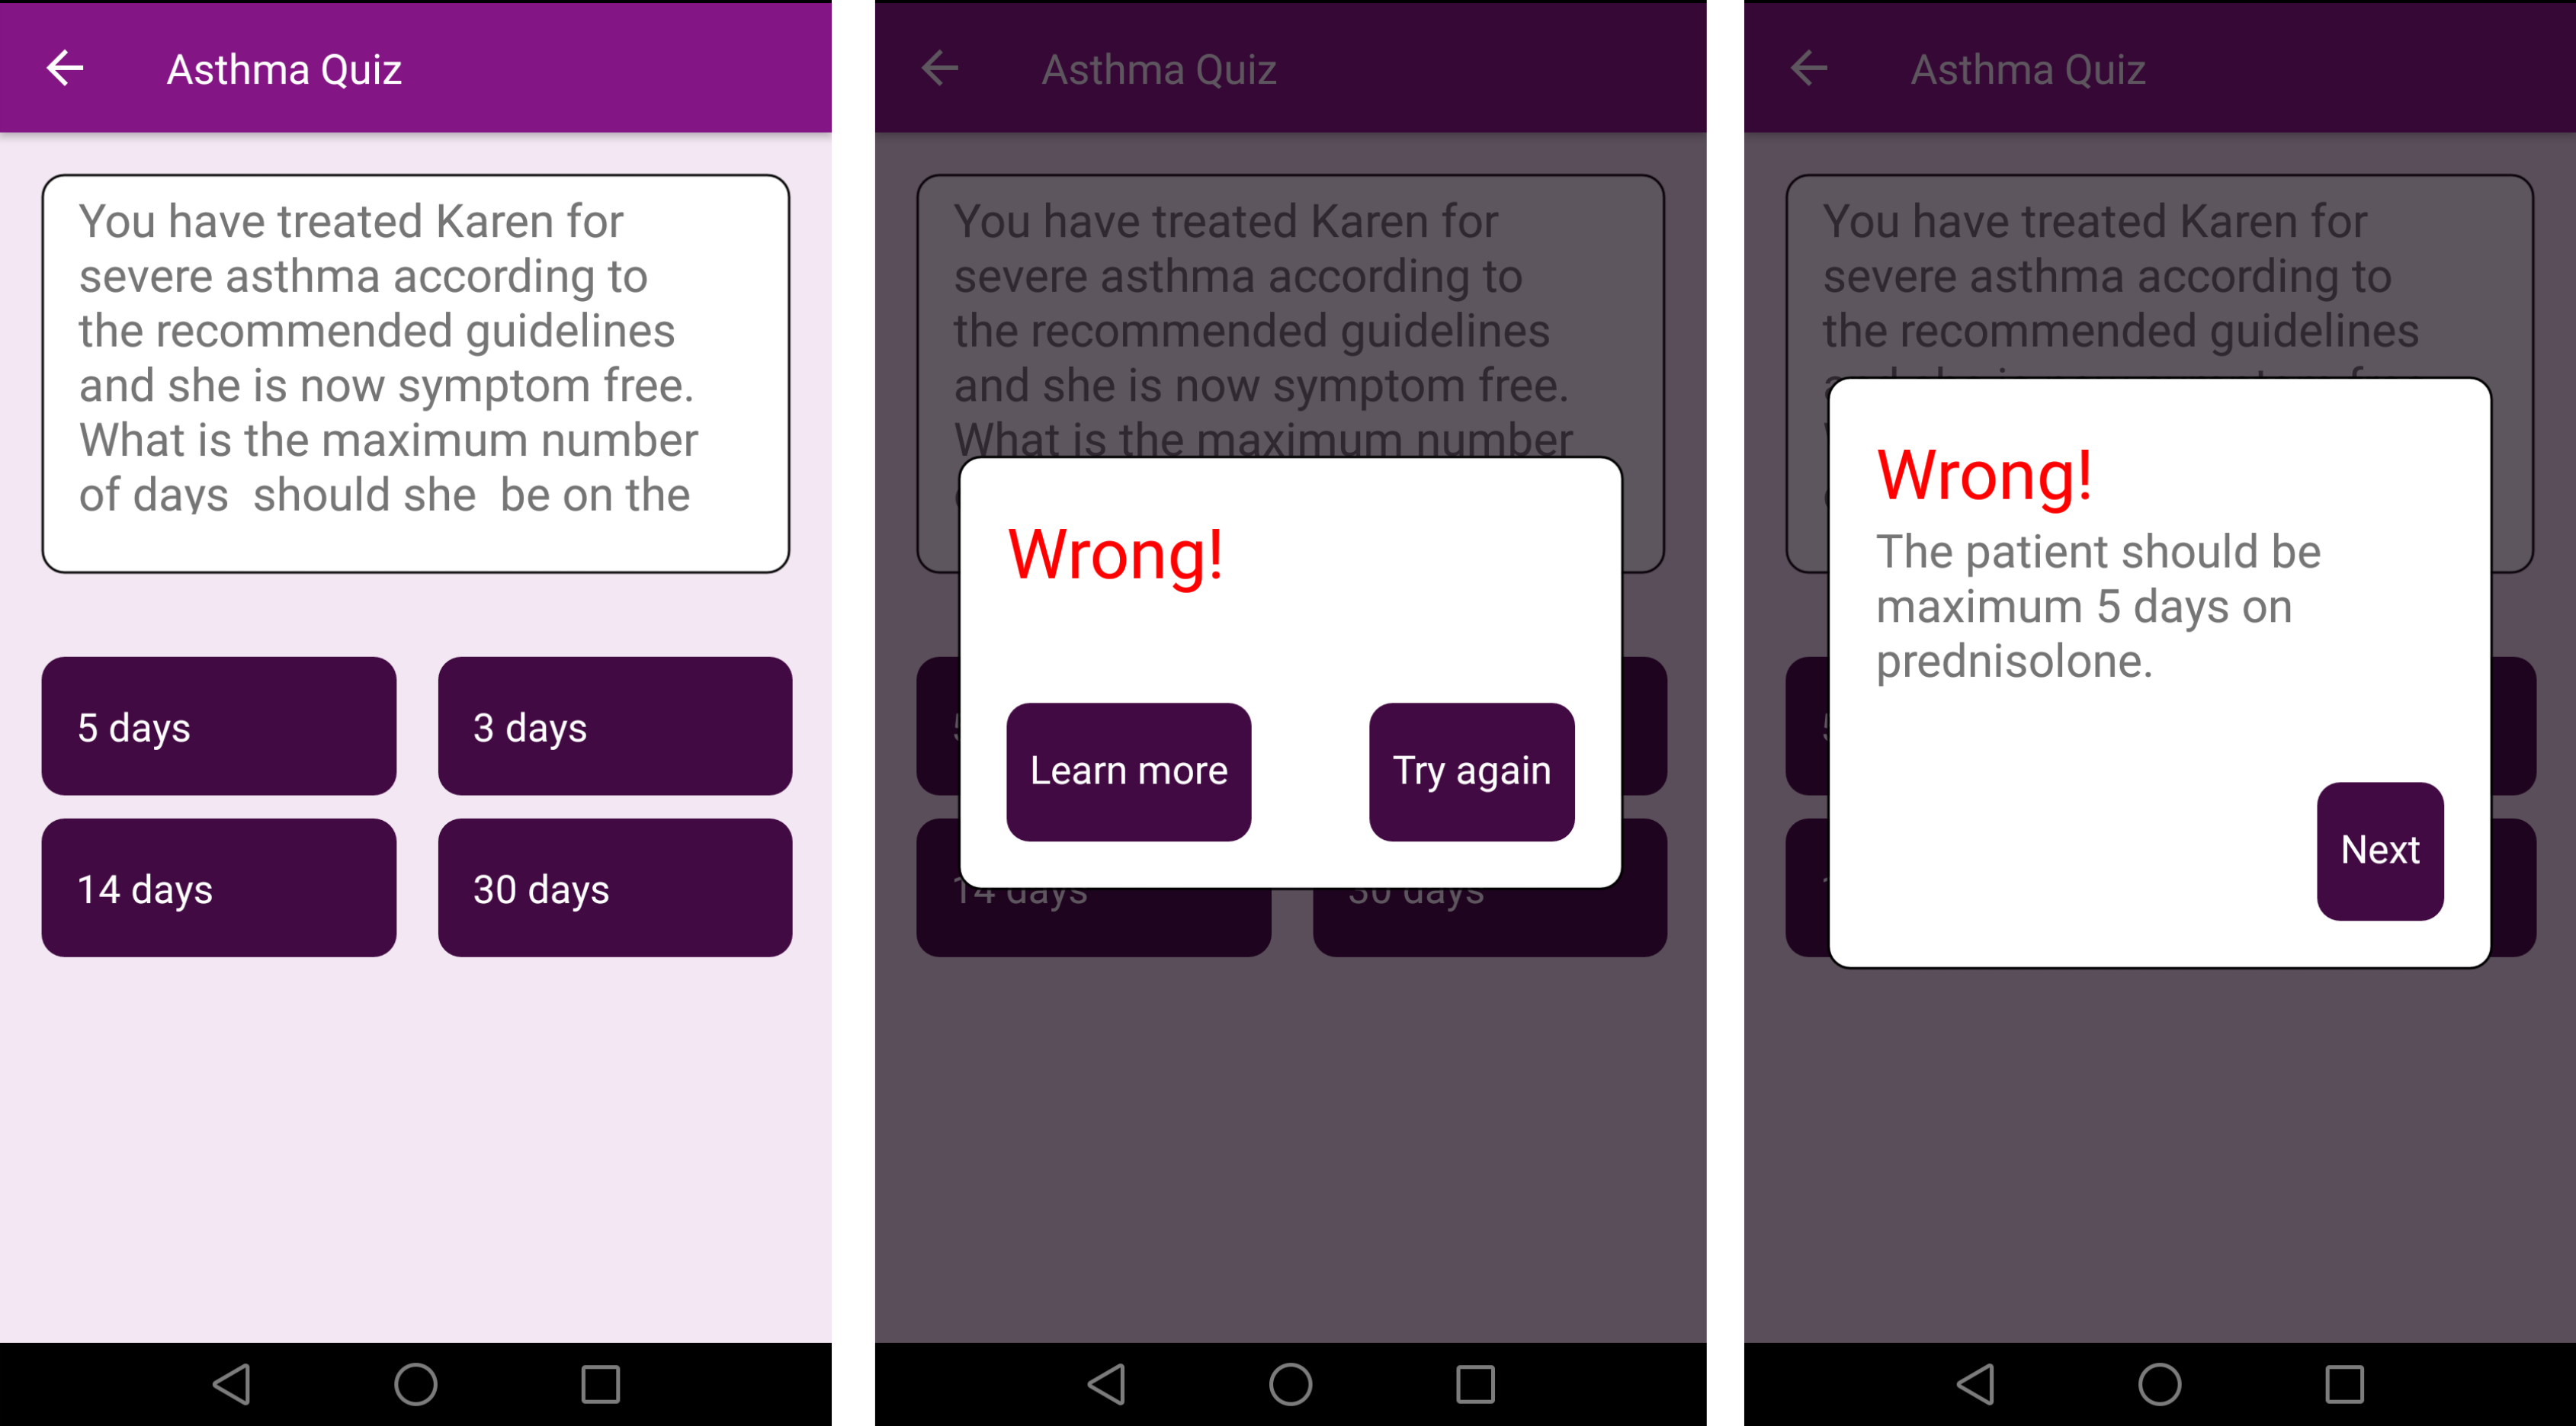
\includegraphics[scale=0.2]{ScreenshotKarenFollowUp}
\end{figure}

When having answered follow-up, which is the last question in the workflow model and the scenario, the student will be presented with his updated position in the student map in figure \ref{fig:ScreenshotLearningMapUpdated}. Brown means previously unlocked levels. Grey means levels which are still locked and green means levels that have been unlocked after this game. If the student performs poorly, red boxes will appear. These boxes indicate that the current level has been locked, and that the student needs to complete quizzes at lower levels to repeat some of the more basic guideline content.

\begin{figure}[h!]
	\caption {After completing the quiz, we are shown the student's updated position in the learning map. The brown background shows levels which has been completed. Grey is the levels which are still unlocked. Green is that we have advanced to the next level. A red box would have indicated that we had performed poorly, the level would have been locked and we have to complete an easier level before we can play it again}
	\label{fig:ScreenshotLearningMapUpdated}
	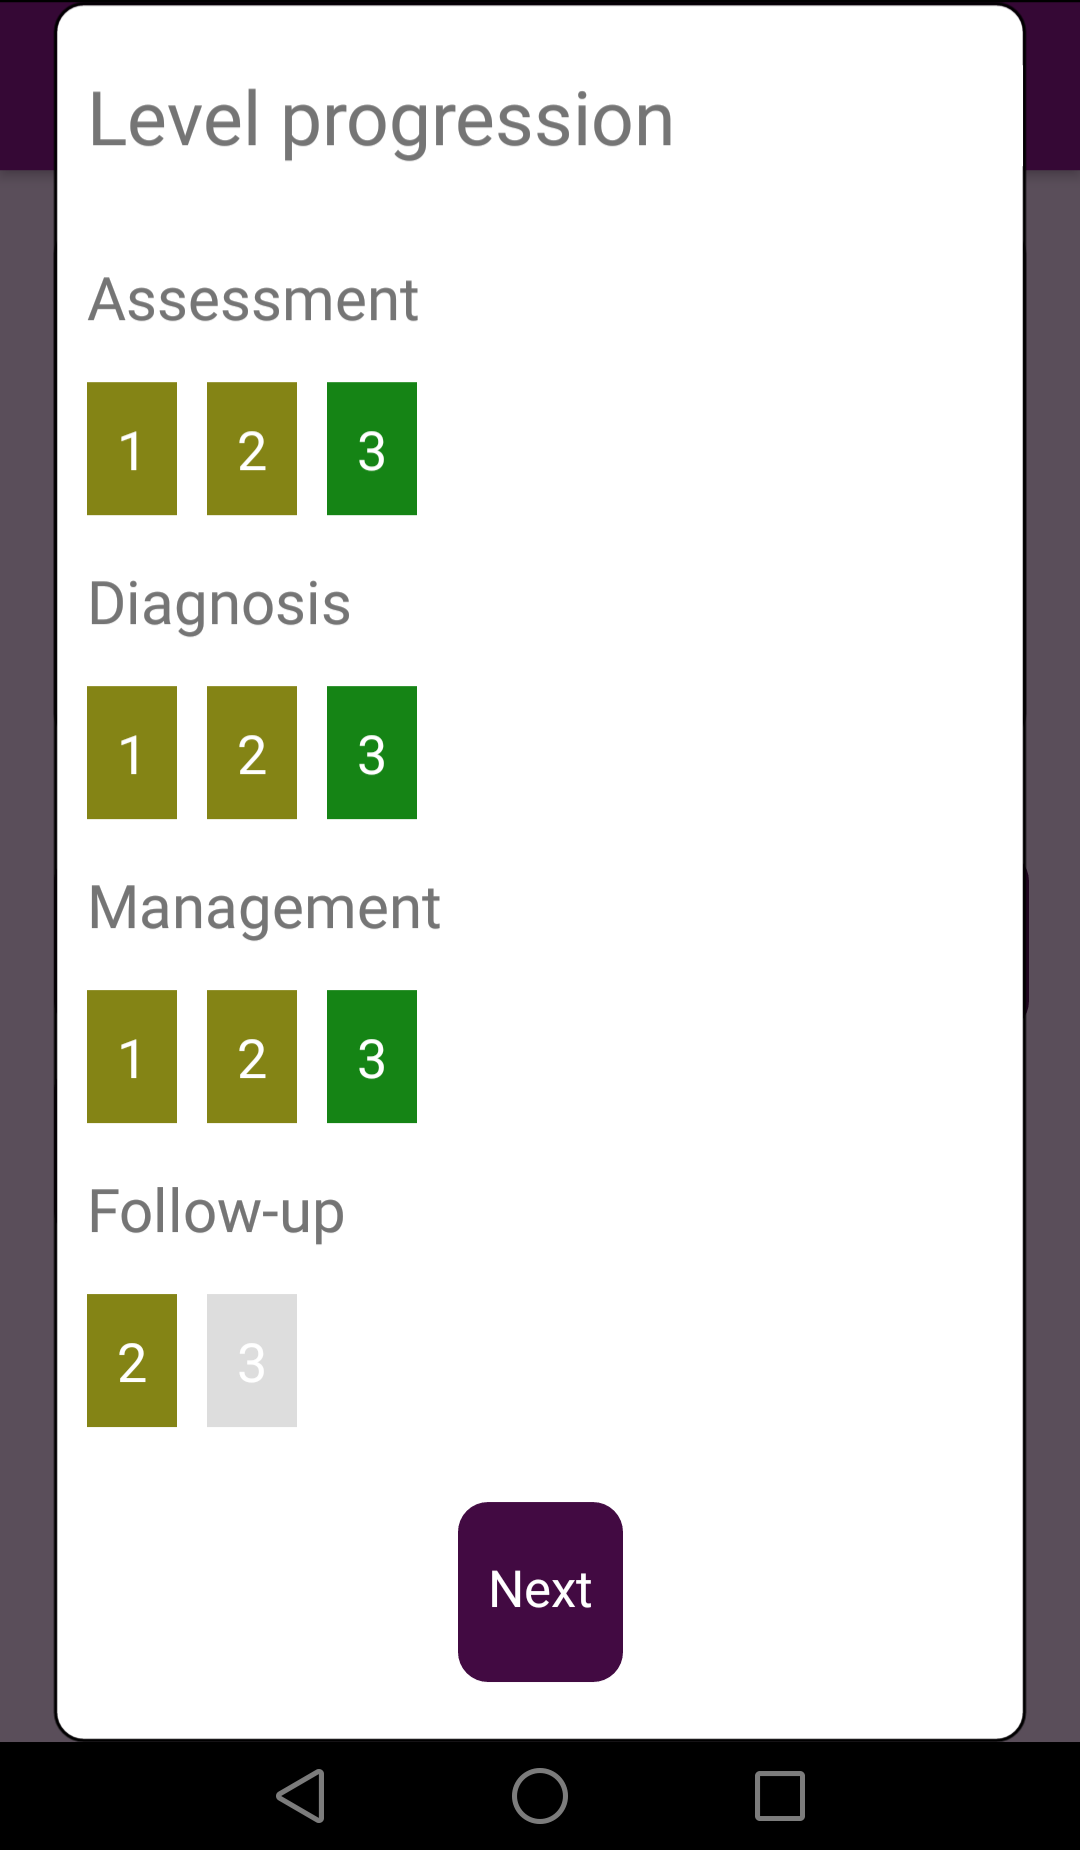
\includegraphics[scale=0.2]{ScreenshotLearningMapUpdated}
\end{figure}

The last screen in this game sequence is shown in figure \ref{fig:ScreenshotHighCharts}. The blue bars show our scores for the questions categorized according to the workflow model. The scores are for the current game we just played. The red lines show the scores needed to complete each category for the current level.

From the learning map and graph, we see that we completed the current level of assessment, diagnosis and management. We didn't complete follow-up, so the next time we play the asthma quiz we will only get questions from level 2 follow-up. The reason why the student won't get questions from assessment, diagnosis and management, is that we don't want to bore the student with continually asking the same questions that we know the student already knows the answers of.

The idea of the chart is to make the student motivated, when he sees his progress getting closer and closer to the red requirement line for every time he plays the asthma quiz at that level. Confirming that he learns more every time.

We used Highcharts \parencite{Highsoft} to display the interactive chart of the game scores and the scores required to complete each category.
\begin{figure}[h!]
	\caption {The bars show our scores for the played game in the different parts of the clinical encounter. The red line shows the scores needed to complete this level}
	\label{fig:ScreenshotHighCharts}
	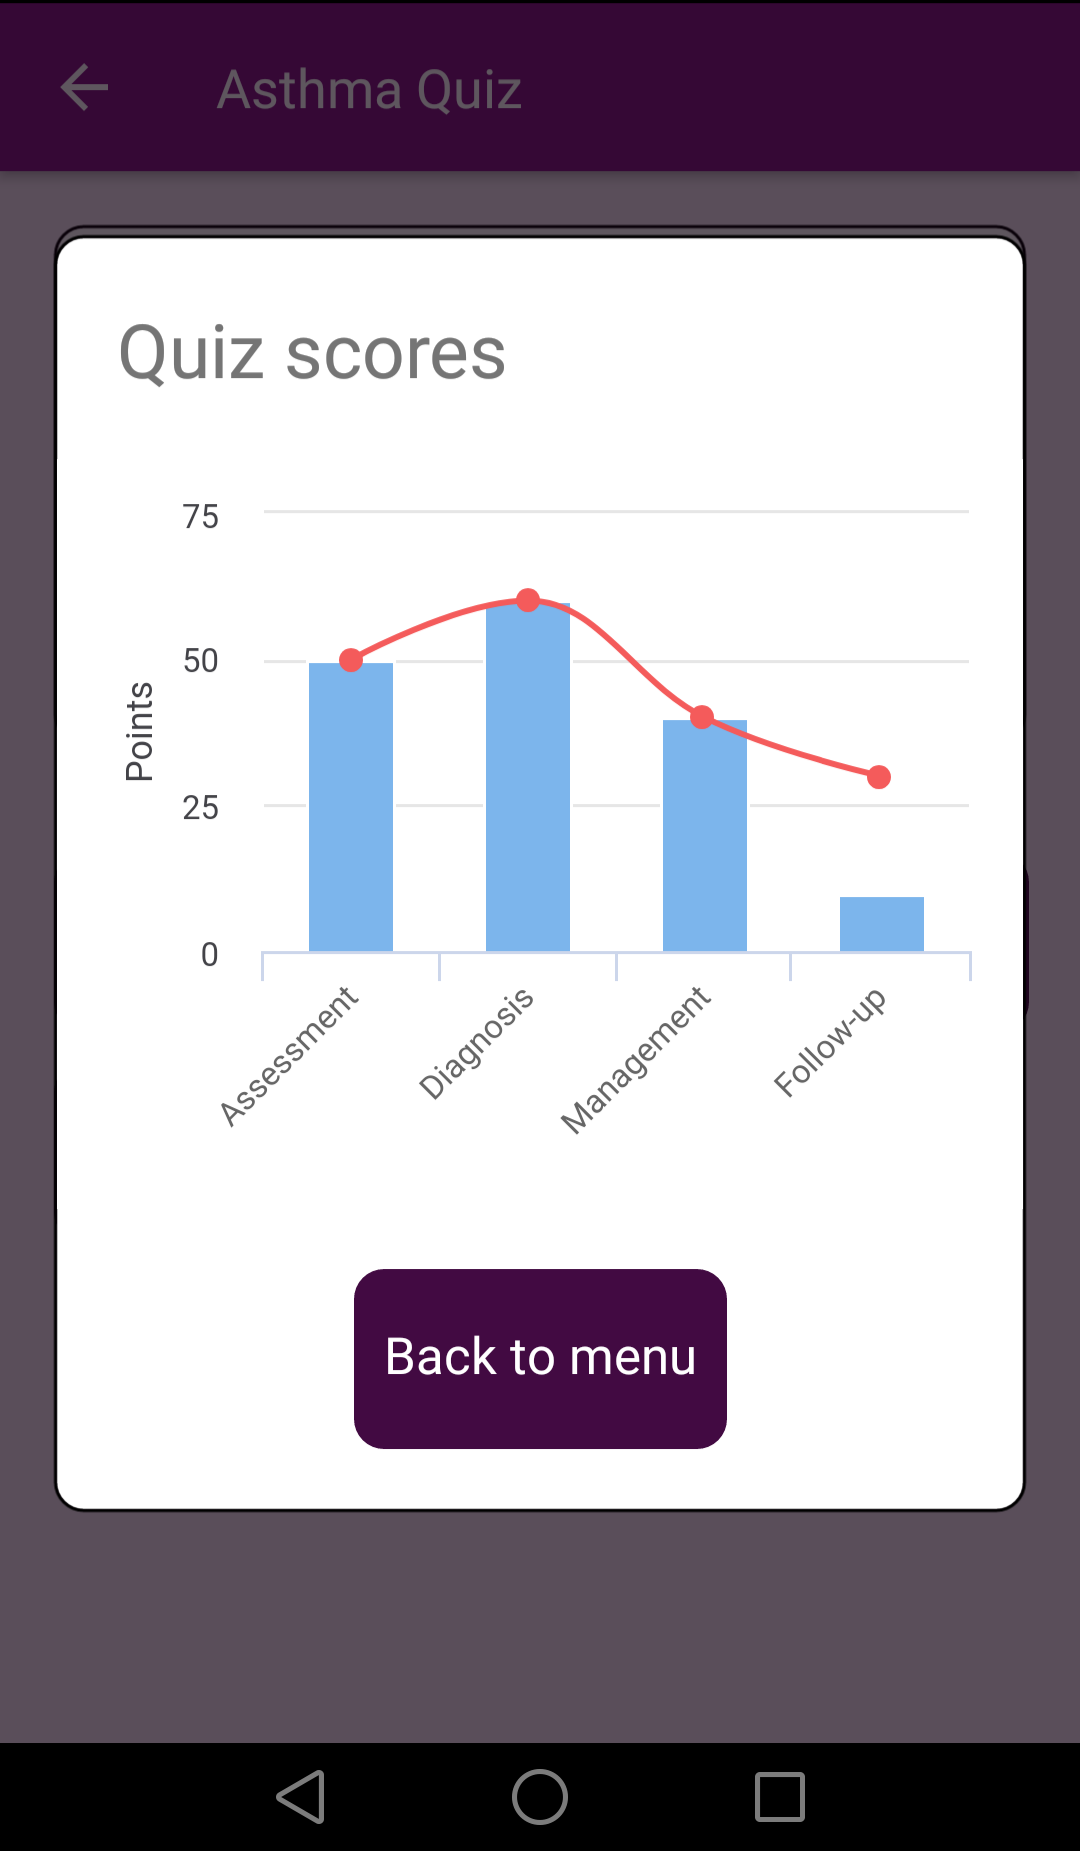
\includegraphics[scale=0.2]{ScreenshotHighCharts}
\end{figure}




\chapter{Discussion}
Right now we have modelled parts of the guideline for prescribing oxygen \parencite{RepublicofKeny2016} and antibiotic administration \parencite{RepublicofKeny2016} into the entity model of the paediatric possible asthma guideline \parencite{RepublicofKeny2016}. This is to be able to ask detailed questions about relevant treatment, as well as making sure that the student knows the basics of the treatment. In a future version we can have separate quizzes for prescribing oxygen and antibiotic administration. We have already applied Dynamic Content Management (DCM) to the asthma quiz, but we can also apply it to a higher abstraction level. We can say that the student needs to complete the quizzes for prescribing oxygen and antibiotic administration, before he is allowed to play the asthma quiz. Then we have a knowledge dependency. According to DCM he can choose whether he wants to complete prescribing oxygen first or antibiotic administration first, but both have to be completed to advance to the paediatric possible asthma guideline.

\section{Research questions}
\section{Evaluation}

\subsection{Evaluation of the models}
To evaluate our model, we have decided to model the paediatric pneumonia guideline \parencite{RepublicofKeny2016}. As we have a strict time limitation it is better for us to evaluate a respiratory condition, as we have already worked with a respiratory condition in asthma. There is quite a lot of work for software developers to learn a new clinical guideline, so we save a lot of time when the concepts are similar.

In figure \ref{fig:PneumoniaEntityGraph} we have modelled the entity model of the paediatric pneumonia guideline \parencite{RepublicofKeny2016}. We see that both guidelines have a history part, where the patient or dependants can tell something about the condition of the patient. Both guidelines also have an examination part where the clinician looks for several symptoms. The symptoms are a bit different from paediatric possible asthma guideline, but they have several symptoms in common. Wheeze is something the clinician has to be aware about. If the patient is wheezing, the patient should be treated according to the paediatric possible asthma guideline instead.

The management part is also quite similar to the paediatric possible asthma guideline. The patient and dependants will be given some advise concerning the medical condition of the patient. If the pneumonia is severe, or the patient has lower chest wall indrawing and the patient cannot be reviewed within 48 hours, the patient should be admitted into the hospital. The medication is quite similar to the paediatric possible asthma guideline. For pneumonia there are fewer medications, but both guidelines have treatment with antibiotics and oxygen.

The big difference is the diagnostic part. For the paediatric possible asthma guideline, there is only one medical condition described. However, for the paediatric pneumonia guideline patients with tuberculosis or HIV will receive a different treatment. We have not modelled the treatment for pneumonia patients with HIV or tuberculosis as they are separate guidelines. But we need to identify such patients and refer to their respective guidelines. The same goes for asthma. Wheezing patients needs to be identified for asthma treatment.

To support several conditions, we have used inheritance on the diagnosis vertex. A new problem occurs as how should we model tuberculosis, no tuberculosis and that we don't know if the patient has tuberculosis? Earlier on, we used the open world principle for the symptoms. If the vertex doesn't exist, we haven't done the examination for the symptom and we don't know if the patient has it or not. The same goes for diagnosis. If the vertex is not there, we need to clarify if the patient has tuberculosis. To model the situation where we know that the patient hasn't tuberculosis, we have introduced the diagnosis "no tuberculosis". An alternative solution could be to introduce an attribute "status". The attribute could hold information about the patient evidently has the condition, evidently don't have the condition and if it is not clarified. A fourth status could be if the condition is recurring.

\begin{figure}[h!]
	\label{fig:PneumoniaEntityGraph}
	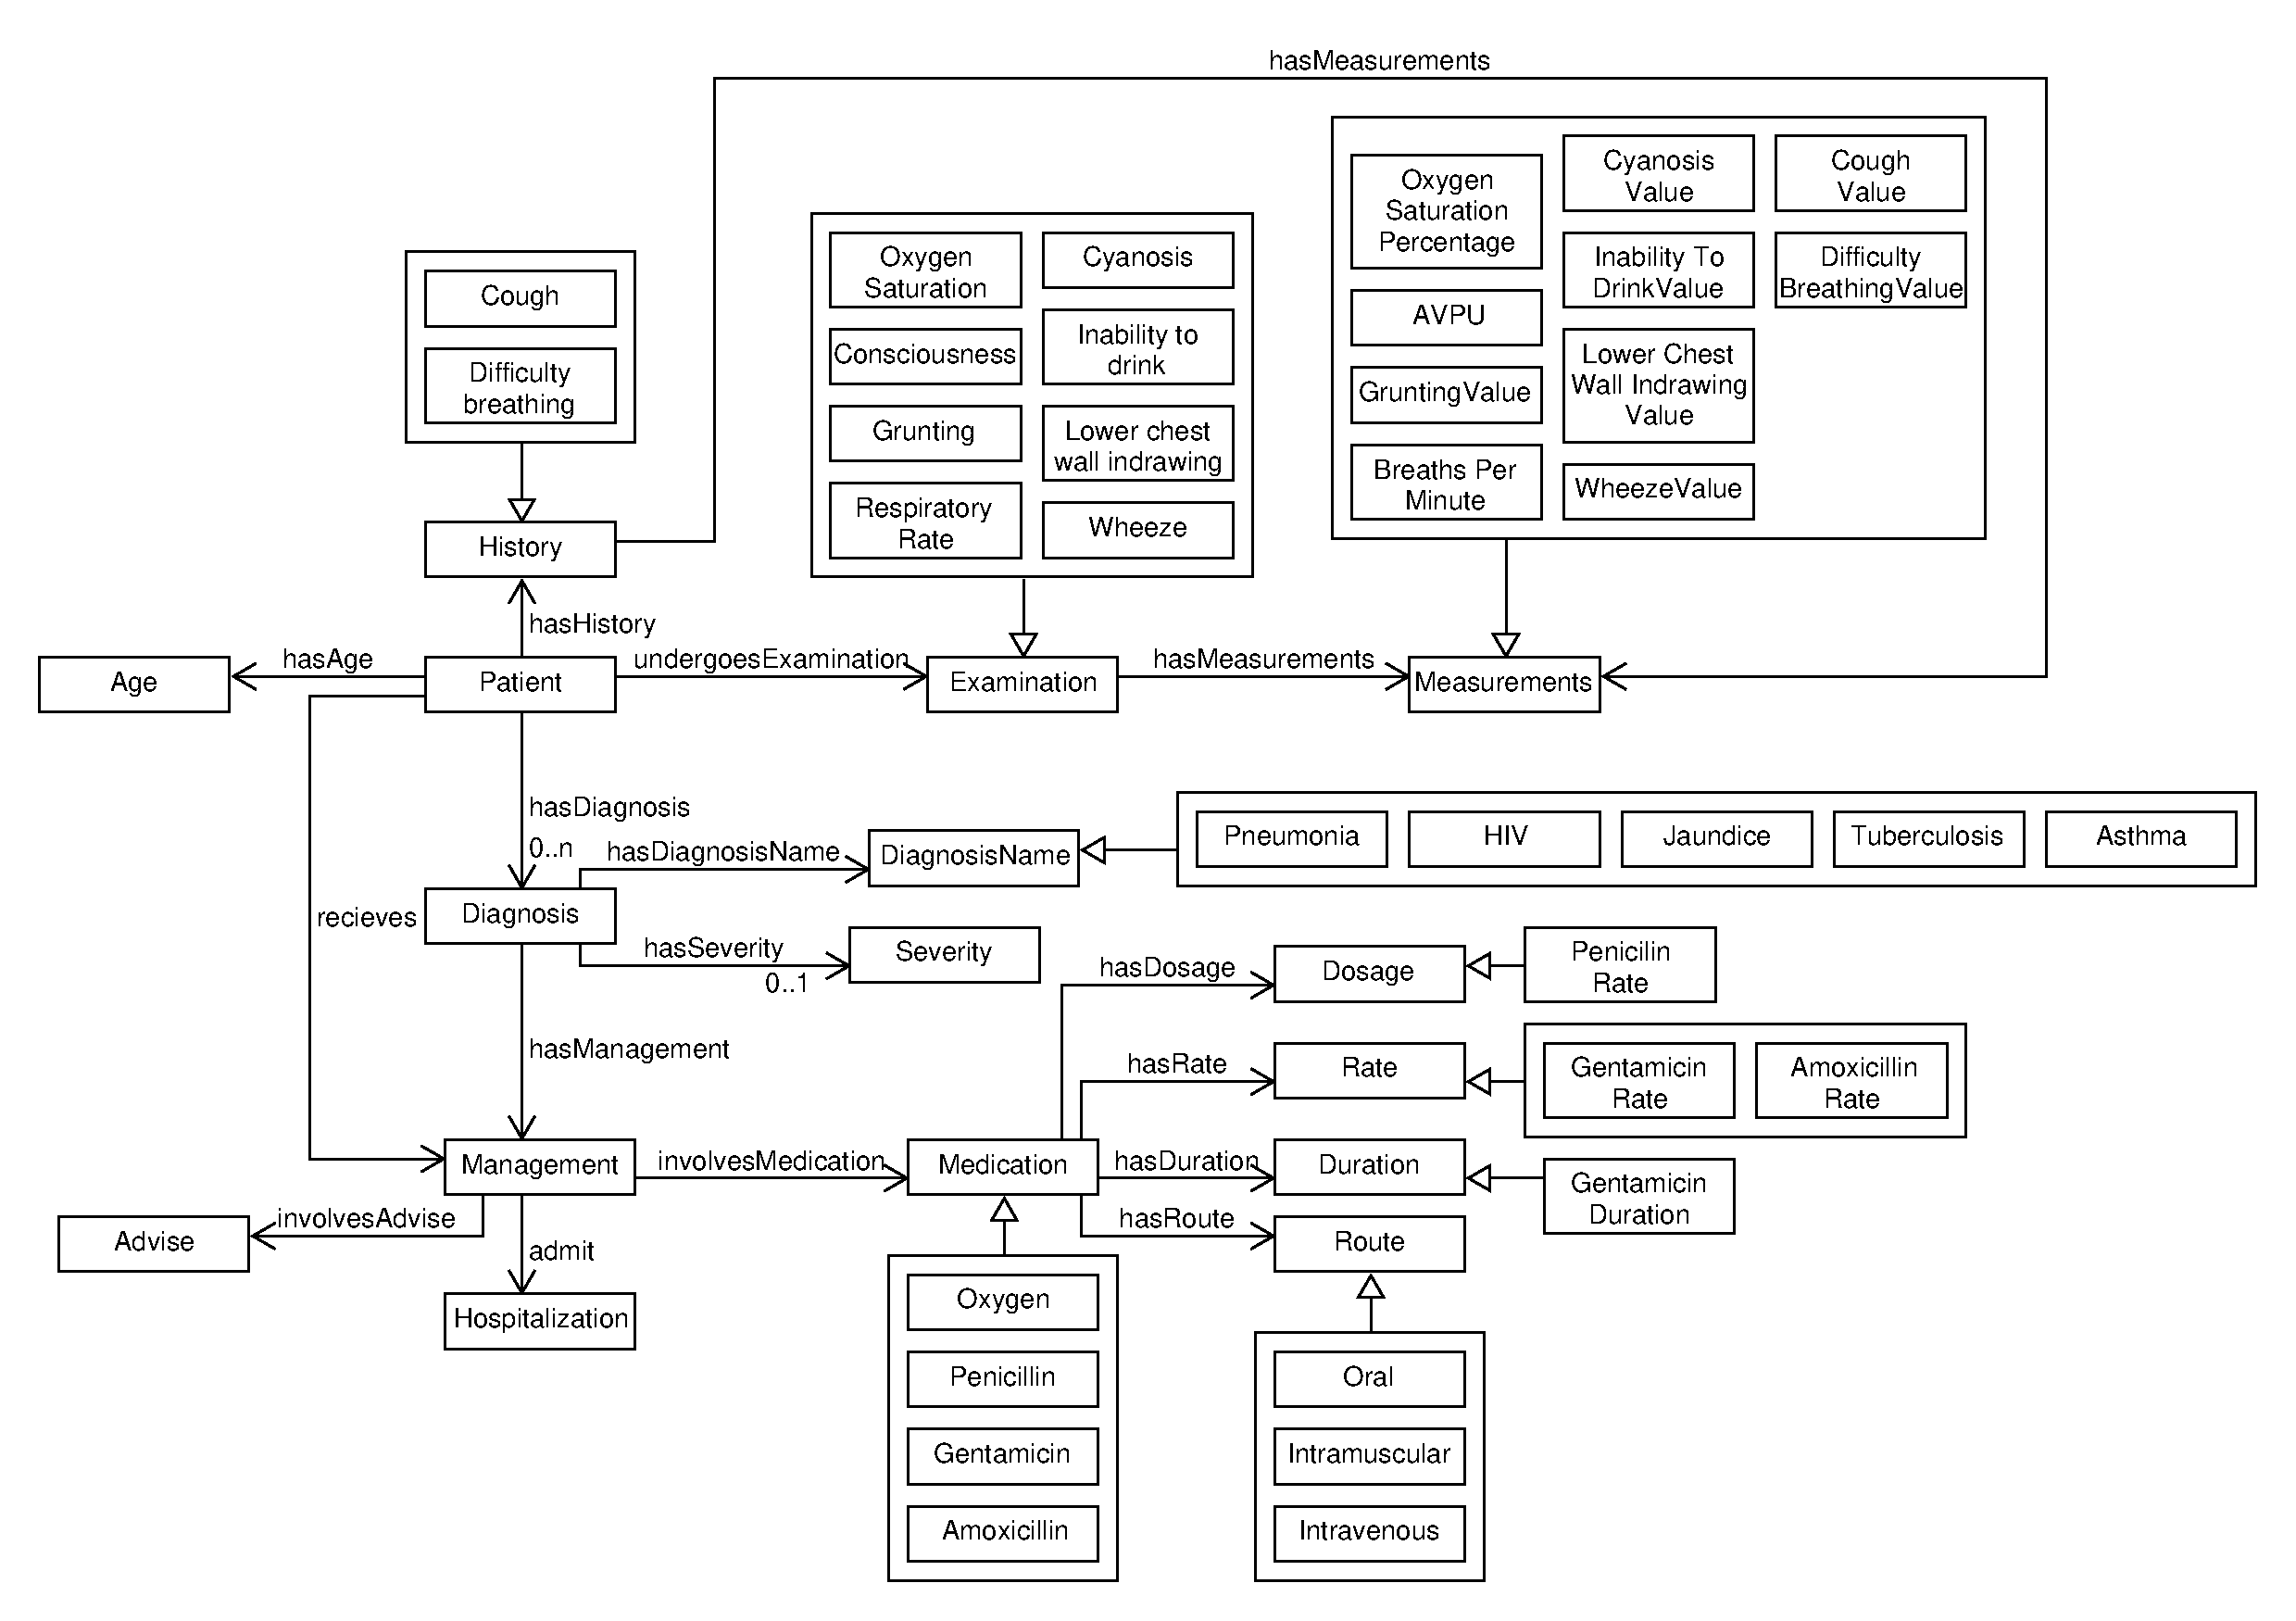
\includegraphics[scale=0.33]{PneumoniaEntityGraph}
	\caption {We are showing that our model is general enough to represent other CPGs. Here we have modelled the paediatric pneumonia guideline \parencite{RepublicofKeny2016}}
\end{figure}

To evaluate the workflow model in figure \ref{fig:WorkflowGraph}, we do like we did for the paediatric possible asthma guideline \parencite{RepublicofKeny2016}. We see the guideline in combination with the entity entity and the workflow model. The paediatric possible asthma guideline \parencite{RepublicofKeny2016} has an assessment part, where we look for patient older than 60 days, cough or difficulty breathing. If he has those symptoms and does not wheeze, we continue looking for other pneumonia symptoms. In the diagnostic part we strengthen our assumption of pneumonia, we set the severity of the diagnosis and we further keep in mind that if the the patient is wheezing he should be given the asthma treatment. Pneumonia patients with HIV or tuberculosis should be referred to specific guidelines for those condition combinations \parencite{RepublicofKeny2016}. In the management part, some patients get admitted into the hospital. The management further has an advise for review within 48 hours. The patients condition is then evaluated either on the hospital for admitted patients, or in a review within 48 hours for other patients. We can conclude with that the workflow model  also covers the paediatric pneumonia guideline \parencite{RepublicofKeny2016}.

In figure \ref{fig:PneumoniaPneumoniaIntegratedEntityWorkflowModels} we demonstrate an instance of the entity model working together with an instance of the workflow model. The patient goes through assessment, diagnosis, management and evaluation. As the patient has jaundice, he won't receive penicillin treatment. As the the pneumonia is severe, the treatment will be evaluated at the hospital and schedule for review is unnecessary. 
\begin{figure}[h!]
	\label{fig:PneumoniaPneumoniaIntegratedEntityWorkflowModels}
	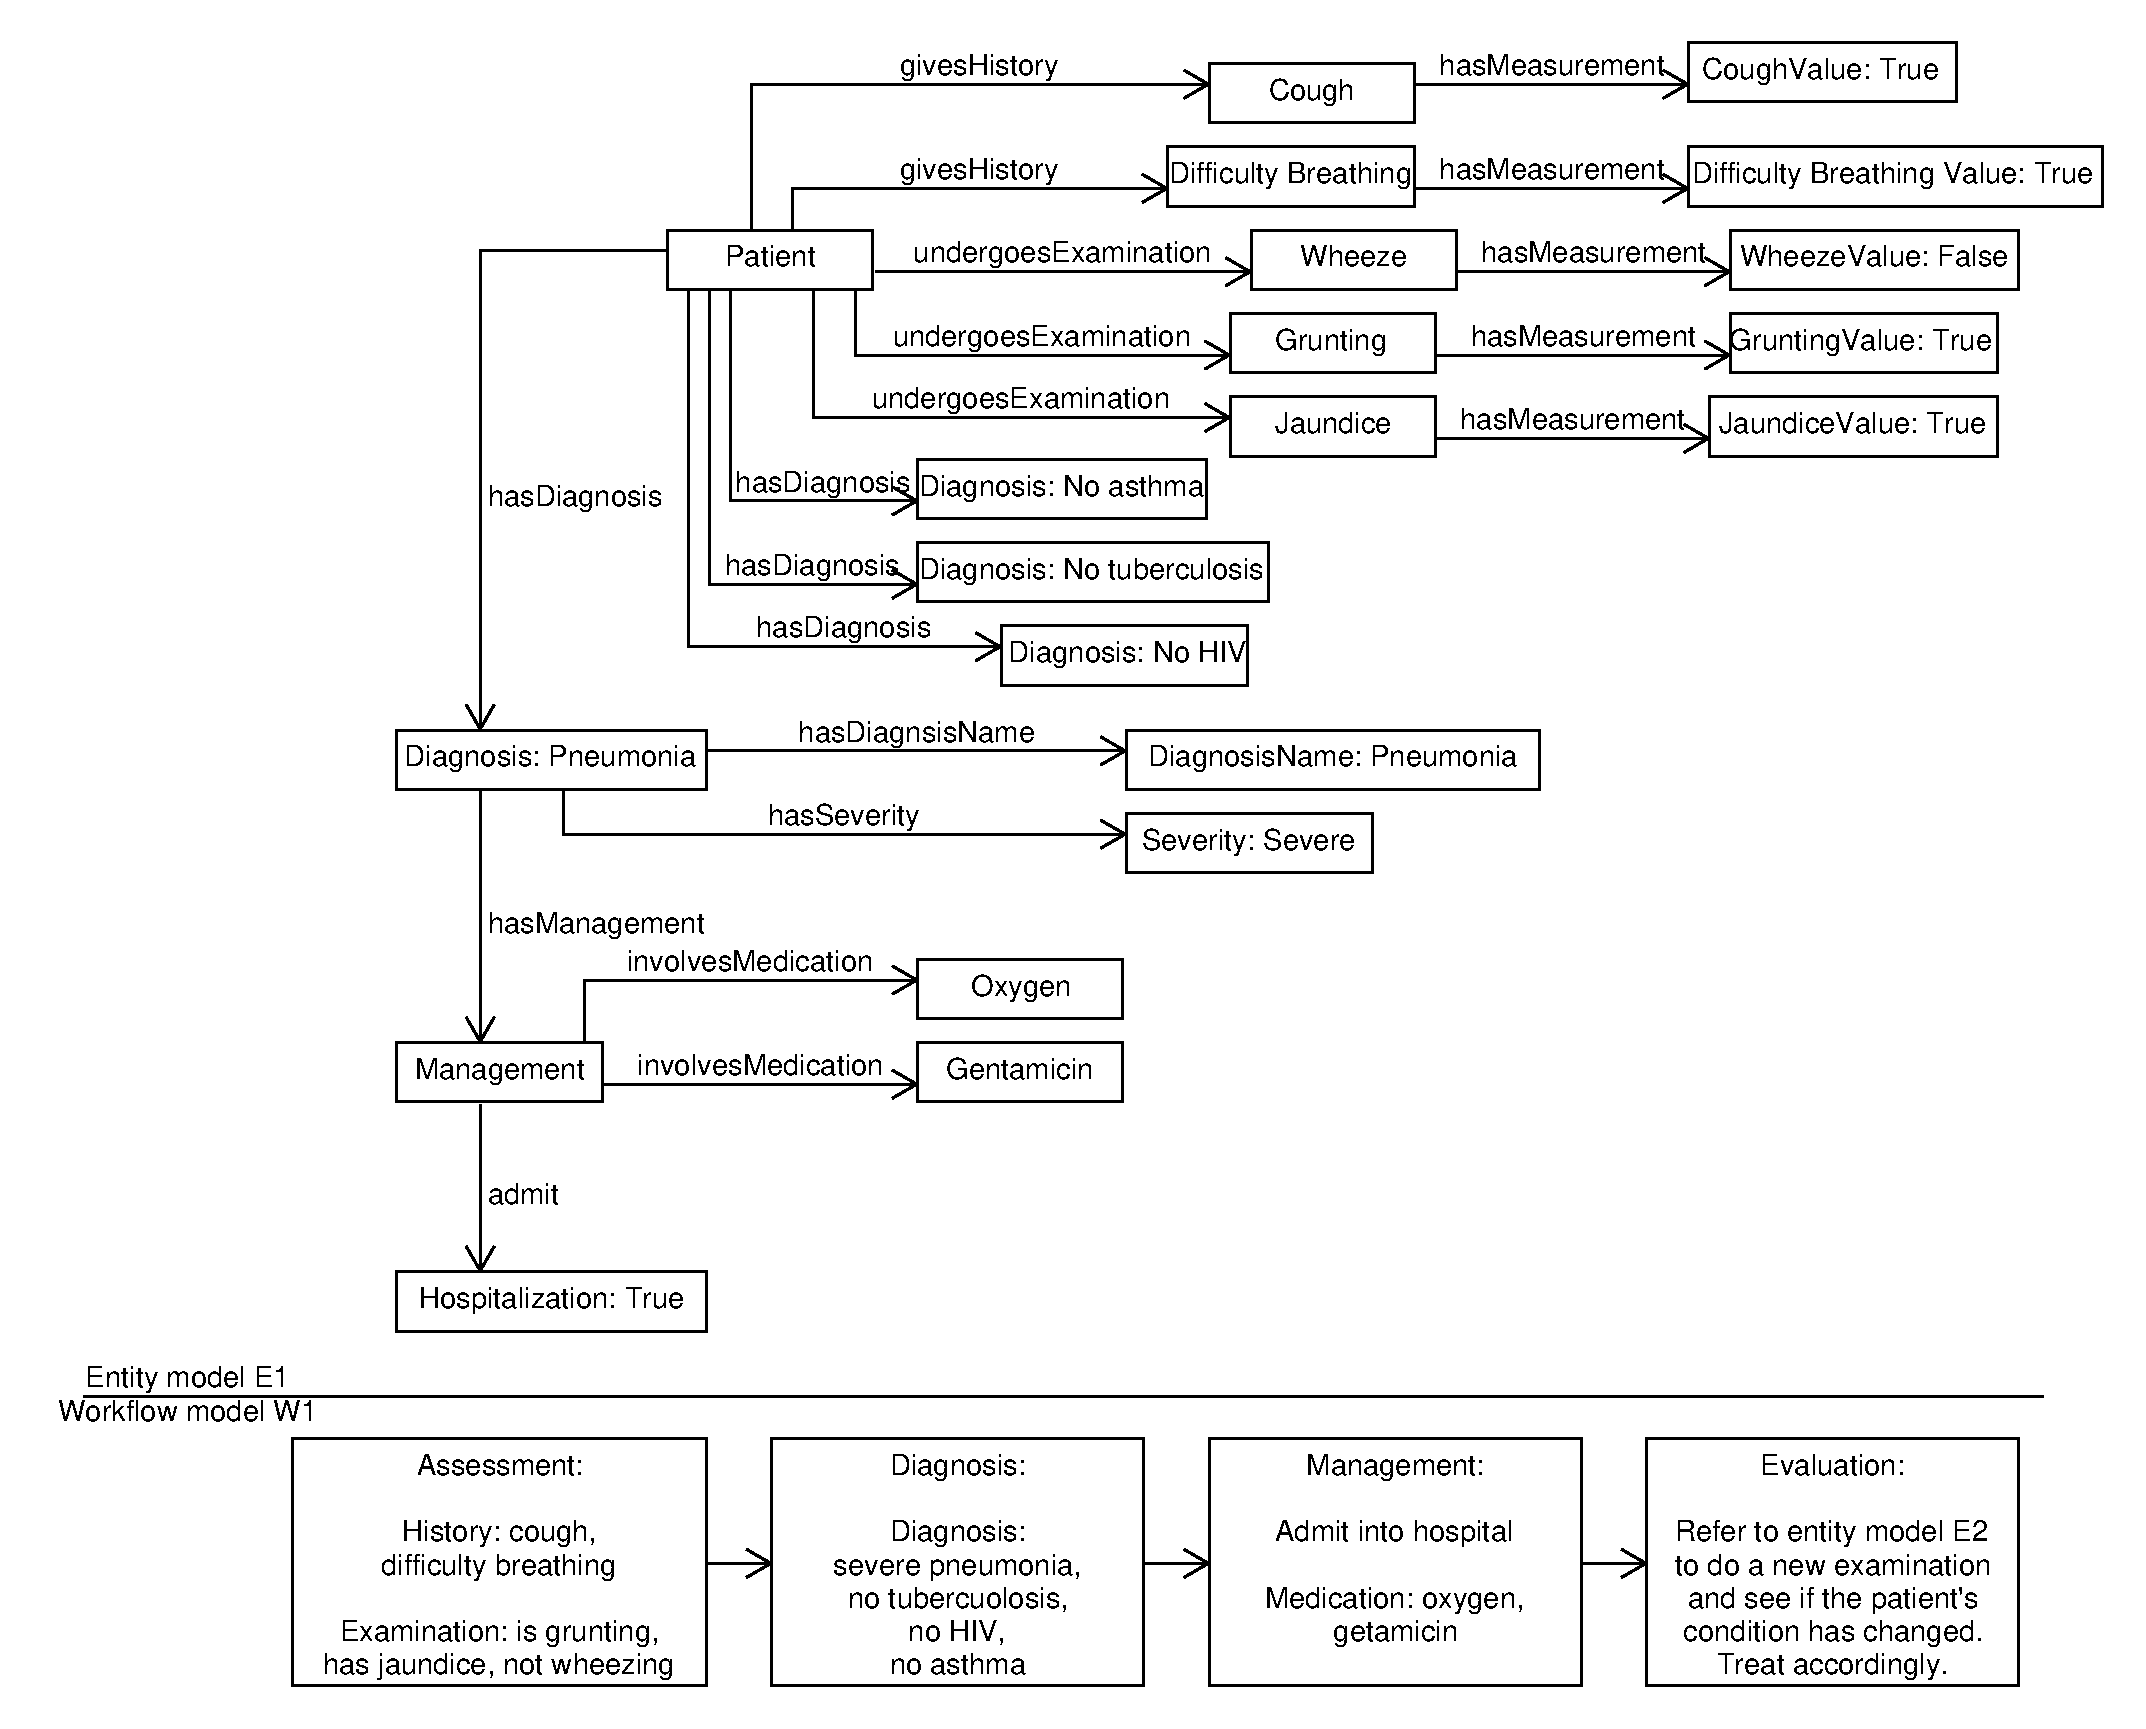
\includegraphics[scale=0.4]{PneumoniaIntegratedEntityWorkflowModels}
	\caption {We are showing out entity model working together with the workflow model for paediatric pneumonia guideline \parencite{RepublicofKeny2016}}	
\end{figure}

After the evaluation, we see that we have modified the entity and workflow models to support both pneumonia and asthma in paediatric medicine. It is likely that further modification and expansion of the entity model is needed when modelling other CPGs. However, we see that we have identified reusable elements of the guidelines, and our models can work as a stepping stone for guideline formalization standardisation.


\subsection{Evaluation of the application}
The evaluation of the application was done with clinicians.	Two medical doctors and two specialist nurses. Both of the specialist nurses are employees at the polyclinic for pulmonary diseases at Haukeland University. One of the nurses is a specialist in sleep apnea, and his master thesis was writing clinical guidelines for sleep apnea. The other nurse is a specialist in asthma, but in adult medicine.

The evaluation method was a combination of the cognitive walkthrough and usability test in controlled environment, with follow-up questions. In detail what we did was, the clinicians would be asked to play the most difficult level of the game, speak what they are thinking when playing the game and manoeuvring in the application. Topics to discuss would occur when the clinicians had to think out loud. The master student would observe and take notes when problems and confusions occurred, or that the clinician expressed emotions such as joy, excitement or disappointment.

\begin{enumerate}
	\item Can the application be a useful learning tool for medical students, nurses and doctors?
	\begin{enumerate}
		\item Very useful indeed. Would be nice to take a test after a lecture about asthma or after having read about asthma to see how much I have learnt and remember. A quiz is far more fun than a check list in paper format. The application is also good for scalability, as you can train a lot of clinicians without adding any resources. Also great if a course leader can see the progress or the level of his students.
		\item Absolutely useful, and I feel I have learnt a lot by just doing this quiz. The nurse found the game to be very engaging, cheering when getting a correct answer. 
	\end{enumerate}
	\item How is the flow of the questions? Is the idea of scenarios where we go from assessment, diagnosis, management and follow-up a good approach?
	\begin{enumerate}
		\item Happy with the float and the use of scenarios.
		\item Very happy with the float, being able to follow the patient from the start to the end of the treatment.
	\end{enumerate}
	\item Did we manage to present the important elements of the asthma guideline?
	\begin{enumerate}
		\item Don't know the asthma guideline well enough to answer that.
		\item Don't know the paediatric asthma guideline well enough to answer that.
	\end{enumerate}
	\item Is the detail level the element to adjust for the difficulties of questions?
	\begin{enumerate}
		\item Yes, but would like to have an even harder level with more details.
		\item Yes, it seems like a right approach. The target group of users is relevant here, that this is meant for the emergency clinic.
	\end{enumerate}
	\item How are the answer key explanations?
	\begin{enumerate}
		\item 
		\item I like how the measurements corresponds and are calculated with the scenario and the patient they are presented with. The answer key explanations gives relevant answers to the questions asked.
	\end{enumerate}
\end{enumerate}

Quality of questions
\begin{itemize}
	\item The assessment, none of the distractions is a wrong answer. Even though wheeze is what we are looking for.
	\item When asking for salbutamol dosage, it is relevant to know where and in which stage of the treatment it is being given. Also saying something about rate or duration can help clarify that.
	\item Very nice that we in some questions change the way we ask. Sometimes we give a diagnosis and asks which symptoms identifies it. Then we give some symptoms and then ask about the diagnosis.
	\item In the assessment part of the scenarios, we tell that clinical encounter happens at the emergency clinic. But we should find a way to amplify it even more, as one of the test persons missed that detail.
	\item Descriptions such as "age > 12 months" is hard for clinicians to read. We should avoid using logical operands.
	\item "Recurrence of asthma" is unclear. Who says that it is recurrent? Is it recurrent when the patient is in the emergency clinic? Does the patient tell that it is recurrent? Is it in the journal?
	\item We have a trick question and we should avoid those. We ask what is not the right way to administer salbutamol to a patient. The answer is oral. The clinician thought the right answer could be one of the other alternatives as an oral version of salbutamol doesn't exist.
\end{itemize}

User interface and game experience
 \begin{itemize}
 	\item All the clinicians were very positive to the multiple-try with hint approach. When they give a wrong answer, they get a new chance to revise the question and correct their answer.
 	\item When the clinicians answer a question incorrectly, they are presented with a "learn more" button. When they click on this button they get presented with an answer key explanation. When they click on "next" they get very surprised and disapointed that were taken to the next question and don't get the chance to get the question right.
 	
 	Here the specialist in asthma had a very interesting suggestion. When she clicks on "learn more", she want an explanation of why that suggestion was wrong or in which situations that answer would have been correct. Then she want to try again to collect the reward. She was noticeably disappointed at the summary when she saw that she was penalized hard for clicking "learn more".
 	\item The clinicians wanted a link or a button to display the clinical guidelines in the screen they were presented with the answer key explanation. Then they can read and learn more.
 	\item The clinicians noticed that they didn't have to remember details from the previous question before they answered the next. That was something they appreciated.
 	
\end{itemize}

\textcolor{red}{Er nødt til å skrive et sammendrag her, sånn at vi klarer å treffe forskningsspørsmålene mye bedre. Skal ha evaluering med en eller to leger på søndag, så det gir mening å forme og spisse dette avsnittet litt mer etter det møtet.}

\section{Limitations of the model}
\begin{itemize}
	\item Can't ask questions like "what are the symptoms for severe asthma?"
	\item Difficult to ask what NOT to do. If the vertex doesn't exist, only an empty string gets returned. Can only be used were we actually have written "don't admit to the hospital" as an example with hospitalization.
	\item \textcolor{purple}{TODO Yngve: Graph QL?}The inheritance makes it difficult to generalize some questions. We can't make a template which asks about the Rate a medicine should be taken with. We need to specifically ask for that medicine. To be able to ask for a general medicine, one solution can be to introduce a new tag which compares the substring of the type of the vertex. Another solution is to use the meta model and not the instance model. We don't use inheritance on diagnosis because of this.
	\item To avoid the problem described in the previous point, we don't use inheritance on Diagnosis. A limitation here is that  
	a patient can only have one diagnosis.
\end{itemize}
	


\section{Observations}
\section{Challenges}
\section{Reflection}



\chapter{Conclusions}
\section{Further research and development}


\backmatter
\printbibliography
% bibliography, glossary and index would go here.


\appendix
\chapter{Comparison of CPG applications}\label{appendix:ComparisonApps}
This appendix shows two comparative tables of applications and websites that display clinical guidelines; one for international applications and one for Norwegian applications. The selection is based on a few articles concerning apps for clinical practice and a search for clinical guideline applications on Google Play.
Helsebiblioteket provides access for Norwegian health workers and students to some of the applications and websites below [1], but users do not explicitly need accounts for this.
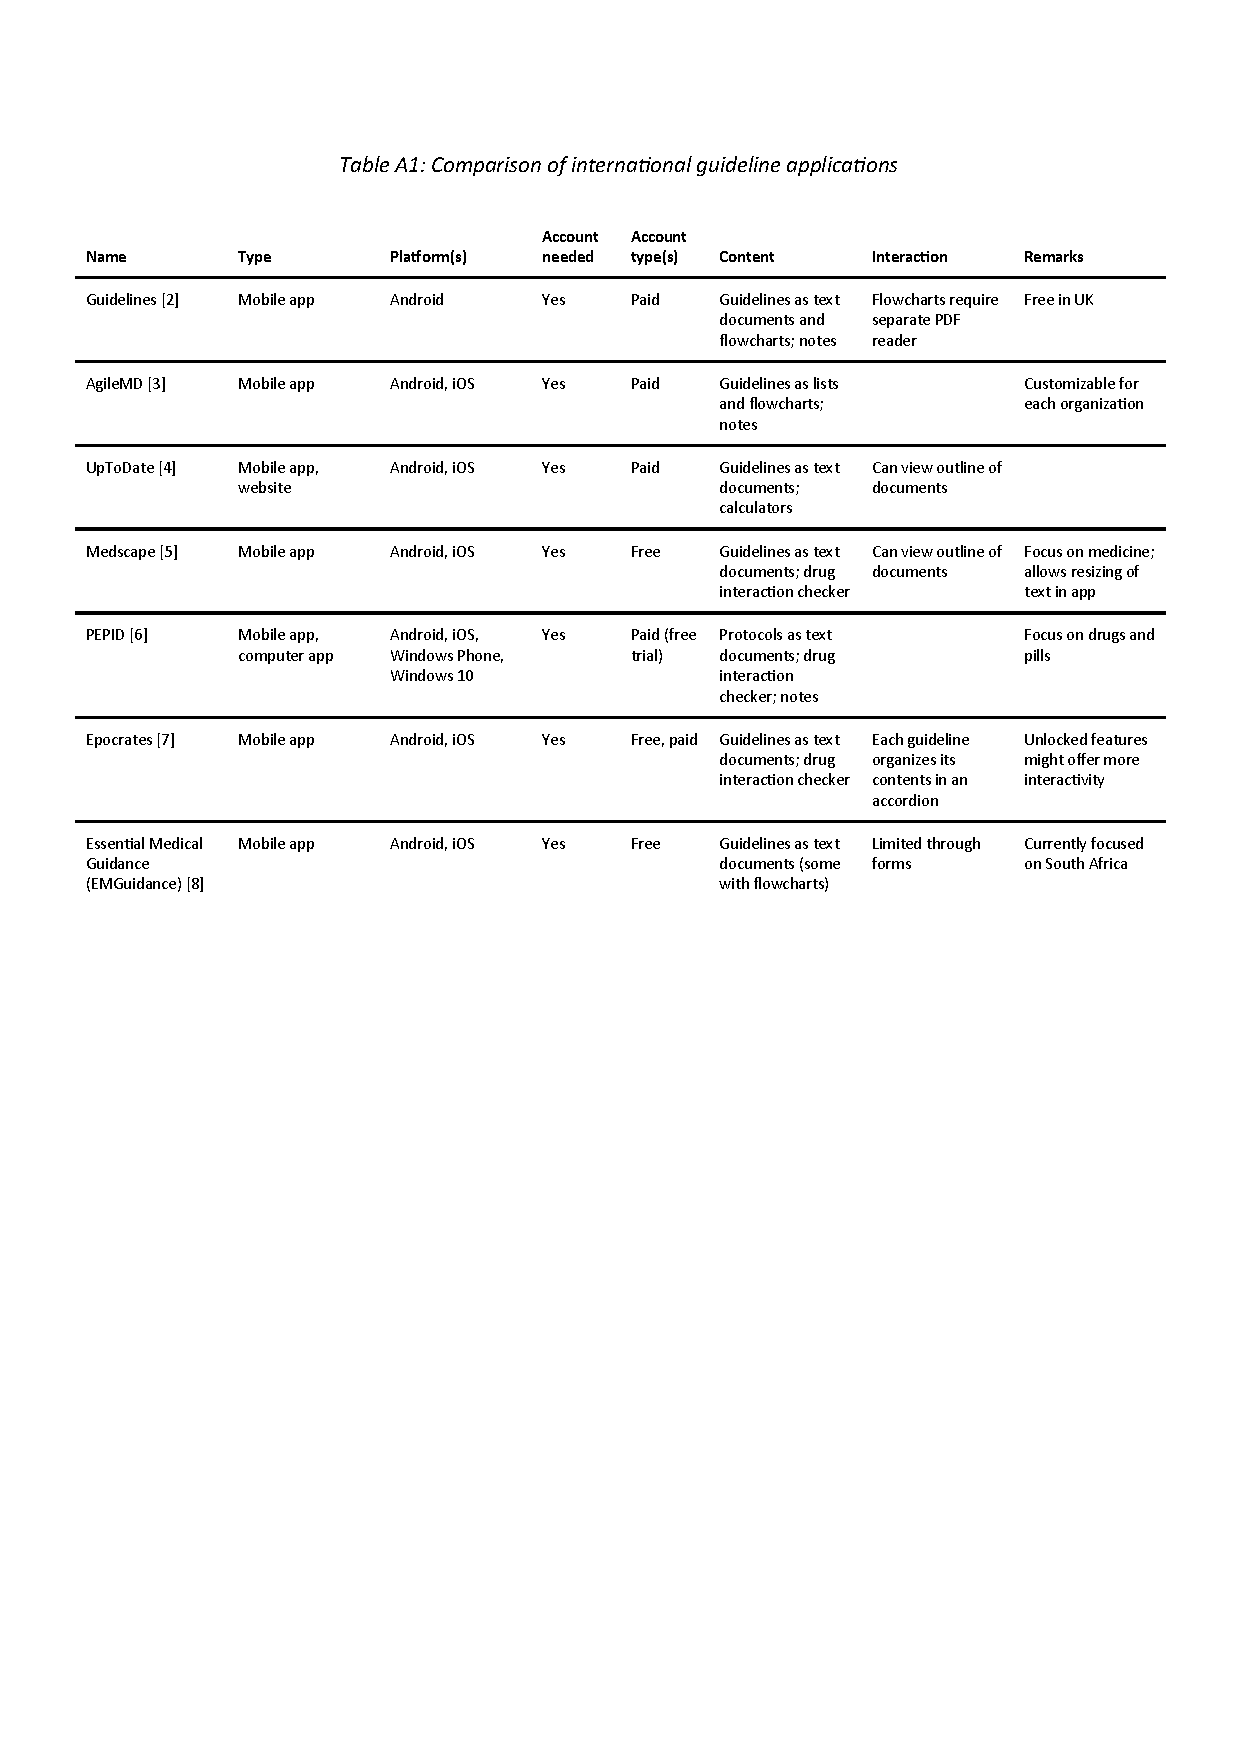
\includepdf[pages={1,2,3,4,5,6,7}]{appendices/comparisonApps}


\end{document}